%package obligatoire : type de document
\documentclass[a4paper,12pt,twoside]{book}
\usepackage{lipsum}

% encodage
\usepackage{fontspec}

% le package hyperref avec des options
\usepackage[pdfusetitle, pdfsubject ={Mémoire TNAH - Numérisation d'un référentiel papier pour indéxation automatique}, pdfkeywords={TNAH, IRHT, Himanis, Trésor des chartes, Archives Nationales, ROC, Numérisation d'instruments de recherche, Alignement de référentiels, REM, REN, Machine learning, Intelligence artificielle, Reconnaissance d'écritures manuscrites, identity linking}, hidelinks]{hyperref}

%il faut mettre au moins une langue
\usepackage[english,french]{babel}
\NoAutoSpaceBeforeFDP % Commenade pour supprimer les espace avant les ":"

% configurer le document selon les normes de l'école
\usepackage[margin=2.5cm]{geometry} %marges
\usepackage{setspace} % espacement qui permet ensuite de définir un interligne
\onehalfspacing % interligne de 1.5
\setlength\parindent{1cm} % indentation des paragraphes à 1 cm
\parskip=5pt %Crée un espace entre les paragraphes pour aérer le texte

\usepackage{lettrine} % lettrines
\usepackage{listings}
\urlstyle{same} % Pour des url soient dans le même style que le reste

%Pour importer des images
\usepackage{subcaption}
\usepackage{graphicx}
\usepackage{float}
\usepackage{chngcntr}
\counterwithout{figure}{chapter} % Pour que les images ne soient pas comptées en fonction des chapitres
\DeclareCaptionFormat{custom}
{%
	\textbf{#1#2}\textit{\small #3}
}
\captionsetup{format=custom} % Améliore le format de légende des images

\pagestyle{plain} % Pour une numérotation des pages sobre

\usepackage[backend=bibtex, sorting=nyt, style=enc]{biblatex}
\FrenchFootnotes
\AddThinSpaceBeforeFootnotes
\addbibresource{Mémoire-TNAH-2022-Reignier.bib}

\author{Virgile Reignier - M2 TNAH}
\title{Vers l’indexation automatique du Trésor des chartes. Constitution, alignement et utilisation d'un référentiel d’entités nommées au sein du projet Himanis.}

\makeatletter
\newcommand{\parttext}[1]{\def\@parttext{#1}}
\def\@endpart{\vskip 0pt plus 0.5fil
	\begin{formatparttext}
		\vspace*{\fill}
		\@parttext % on imprime le texte spécifique à une partie
		\gdef\@parttext{}% on vide le texte spécifique à une partie
		\vspace*{\fill}
	\end{formatparttext}
	\vskip 0pt plus 0.5fil
	\newpage
	\if@twoside
	\if@openright
	\null
	\thispagestyle{empty}%
	\newpage
	\fi
	\fi
	\if@tempswa
	\twocolumn
	\fi}
\makeatother

\newenvironment{formatparttext}{}{}

% DOCUMENT

\begin{document}
	\begin{titlepage}
		\begin{center}
			
			\bigskip
			
			\begin{large}				
				ÉCOLE NATIONALE DES CHARTES\\
				UNIVERSITÉ PARIS, SCIENCES \& LETTRES
			\end{large}
			\begin{center}\rule{2cm}{0.02cm}\end{center}
			
			\bigskip
			\bigskip
			\bigskip
			\begin{Large}
				\textbf{Virgile Reignier}\\
			\end{Large}
			%selon le cas
			\begin{normalsize} \textit{licencié.e ès histoire}\\
				\textit{diplômé.e de master mondes médiévaux}
			\end{normalsize}
			
			\bigskip
			\bigskip
			\bigskip
			
			\begin{Huge}
				\textbf{Vers l’indexation automatique du Trésor des chartes}\\
			\end{Huge}
			\bigskip
			\bigskip
			\begin{LARGE}
				\textbf{Constitution, alignement et utilisation d'un référentiel d’entités nommées au sein du projet Himanis}\\
			\end{LARGE}
			
			\bigskip
			\bigskip
			\bigskip
			\begin{large}
			\end{large}
			\vfill
			
			\begin{large}
				Mémoire 
				pour le diplôme de master \\
				\og{} Technologies numériques appliquées à l'histoire \fg{} \\
				\bigskip
				2022
			\end{large}
			
		\end{center}
	\end{titlepage}
	
	\thispagestyle{empty}	
	\cleardoublepage
	
	\frontmatter
	\chapter{Résumé}
	\medskip
	Blablabla résumé du mémoire.\\
	
	\textbf{Mots-clés~:} TNAH, IRHT, Himanis, Trésor des chartes, Archives Nationales, ROC, Numérisation d'instruments de recherche, Alignement de référentiels, REM, REN, Machine learning, Intelligence artificielle, Reconnaissance d'écritures manuscrites, identity linking.
	
	\textbf{Informations bibliographiques~:} Reignier Virgile, \textit{Vers l’indexation automatique du Trésor des chartes. Constitution, alignement et utilisation d'un référentiel d’entités nommées au sein du projet Himanis}, mémoire de master \og{}Technologies numériques appliquées à l'histoire\fg{}, dir. Dominique Stutzmann et Thibault Clérice, École nationale des chartes, 2022.
	
	\chapter{Remerciements}
	
	\lettrine{B}lablabla remerciements\dots
	
		Faire une liste des abréviations avec : REN, TAL, REM, IRHT, BVMM, EAD, TEI, XML, XSL, CNRS, CTHS, API
		
		Utiliser package %\\usepackage{acro}
		%\DeclareAcronym{api}{short = API, long = Application Programming Interface}
		%\DeclareAcronym{da}{short = DA, long = Département des Archives %Professionnelles}
		%puis on print avec printglossary[type=\acronymtype]
	
	\printbibliography
	
	\chapter{Introduction}
	
	\begin{quotation}
		
	A ce sujet papa avait une plaisanterie. (...) Il disait, quand il présentait maman, « je l’ai connue et épousée à Paris » et (...) il attendait avant de dire « Texas » que tout le monde ait cru, que tout le monde ait pensé qu’il parlait de Paris, France. Ça faisait tordre de rire toutes les fois.
	
	\end{quotation}
	\bigbreak
	
	
	\lettrine{S}{i} le mot \og Paris\fg{} évoque en premier lieu la capitale française, il désigne également d'autres villes à travers le monde. C'est en exploitant l'homonymie entre cette première et une ville du Texas que la citation ci-dessus, extraite du film \textit{Paris, Texas} (1984) de Wim Wenders, construit la plaisanterie. L'information \og Paris\fg{} ne suffit en effet pas à identifier le lieu où lesdits parents se sont rencontrés. Utilisé seul, le mot est naturellement associé à la France. C'est seulement en précisant l'État dans lequel la ville se situe que l'on peut identifier le lieu exact où les protagonistes se sont rencontrés et mariés. Ce jeu d'ambiguïté manifeste ainsi d'une difficulté rencontrée dans le langage naturel : l'identification des références utilisées. La connaissance lexicale ne suffit en effet pas à elle seule pour comprendre un discours, il faut également que les références soient comprises et associées à une réalité clairement identifiée.
	
	Cet enjeu est également présent au sein du TAL (Traitement Automatique des Langues) à travers la notion d'Entité Nommée qui désigne une expression linguistique qui se réfère à une entité unique de façon autonome\footnote{Sur la définition des entités nommées, \textit{cf}. \cite[p. 167--170]{ehrmann_les_2008}.}. L'analyse du contenu textuel a ainsi largement progressé ces dernières années autour de cette notion par le développement de deux techniques : la REN (Reconnaissance d'Entités Nommées) qui consiste à repérer ces objets textuels et à leur attribuer une catégorie et le liage d'entités qui permet d'associer ces objets textuels à un élément décrit par une ressource référentielle. Si un grand nombre de ces travaux concernent des corpus contemporains, quelques chercheurs s'intéressent également à leur application pour la lecture des archives anciennes et rencontrent ainsi les recherches menées par les spécialistes de ces corpus.
	
	\subsection*{Contexte scientifique de travail}
	
	L'Institut de Recherche et d'Histoire des Textes (IRHT) est un laboratoire de recherche fondé en 1937 par Félix Grat et rattaché au CNRS dans le but de faciliter l'accès des chercheurs aux manuscrits et imprimés anciens\footnote{Sur la fondation de l'IRHT, \textit{cf}. \cite{holtz_les_2000}.}. Les recherches qui y sont menées portent également sur la transmission des textes et l'étude des écritures et connaissent à ce titre des développements récents à propos de la lecture automatique des documents anciens. Initiés par sa collaboration au sein du projet GRAPHEM, les travaux en \og paléographie artificielle\fg{} développés par la section de paléographie latine sont menés conjointement avec des chercheurs en informatique spécialisés dans l'analyse de l'image. Les projets développés prennent deux directions principales : la caractérisation des écritures médiévales (Oriflamms, ECMEN, CrEMe) d'une part et la lecture automatique des archives (Himanis, HOME, HORAE) d'autre part. Pilotés par Dominique Stutzmann, ces recherches ont permis le développement d'outils informatiques et de modèles d'intelligence artificielle qui ont largement renouvelé l'accès aux textes anciens.
	
	Parmi les corpus étudiés par ces travaux, le Trésor des chartes occupe une place centrale puisqu'il constitue le matériel source du projet Himanis et participe à celui du projet HOME. Conservé au sein de la série JJ des Archives Nationales, ce fonds se compose d'une immense collection de titres rassemblée par les rois de France. Il se présente sous la forme de registres contenant des actes organisés de manière plus ou moins systématique et linéaire\footnote{Sur la constitution du Trésor des chartes, \textit{cf}. \cite{potin_mise_2007}}. Le projet Himanis (HIstorical MANuscript Indexing for user-controlled Search) a ainsi permis de numériser les registres et de convertir les inventaires et éditions disponibles afin de les structurer en un format homogène et unique\footnote{Les registres numérisés ont été intégrés à la Bibliothèque Virtuelle des Manuscrits Médiévaux \cite{noauthor_bvmm_nodate}. Tous les fichiers issus de ces travaux sont disponibles ici : \url{https://github.com/oriflamms/himanis}.}. Ces éléments ont ensuite servi de base au développement d'un modèle d'indexation automatique des mots présents dans le corpus\footnote{\cites{stutzmann_recherche_2017}. Les résultats sont disponibles dans l'interface \cite{noauthor_himanis_nodate}.}. Par la suite, le projet HOME (History of Medieval Europe) s'est proposé d'amplifier et de généraliser ce travail, en numérisant de nouveaux documents, en associant chaque texte aux données disponibles les concernant et en déposant les résultats dans une plateforme librement accessible \footnote{\url{https://github.com/oriflamms/Home}}.
	
	\subsection*{Problématique du stage}
	
	Ces différents travaux ont ainsi permis de diffuser largement les textes qui composent le Trésor des chartes et de progresser dans l'analyse automatique des écritures qu'ils contiennent. Il reste néanmoins une problématique à approfondir : l'identification des références utilisées au sein des documents. Si les travaux réalisés permettent de faciliter la lecture des textes, cette dernière se trouve encore freinée par la difficile compréhension des références utilisées. Après des travaux récents portant sur la REN dans les chartes médiévales \footcite{torres_aguilar_named_2021}, l'objectif poursuivi est de parvenir à développer un modèle de liage d'entités afin d'enrichir et de désambiguïser les entités nommées reconnues dans ces documents. 
	
	C'est dans ce contexte que mon stage, effectué dans le cadre du Master 2 Archives - Technologies Numériques Appliquées à l'Histoire de l'Ecole Nationale des Chartes, s'est donné pour mission de rassembler les éléments disponibles au sein des données issues du projet Himanis pour avancer sur la problématique de l'identification des entités nommées. A partir des inventaires déjà convertis, des registres numérisés et des travaux préliminaires en REM (Reconnaissance d'Écritures Manuscrites) et REN, nous avons ainsi travaillé sur la construction d'un référentiel et d'une méthode de travail pour lier les entités nommées reconnues en limitant au maximum les ambiguïtés possibles. Le présent mémoire se propose donc de décrire les travaux effectués et la manière dont ils s'insèrent dans un contexte de travail. Nous étudierons les apports des données fournies par les projets Himanis et HOME pour apprendre à désambiguïser automatiquement les entités nommées reconnues dans un texte médiéval. Nous aborderons pour cela les différentes étapes de construction du référentiel ainsi que les difficultés rencontrées dans ce cadre et dans son utilisation.
	
	Dans cet objectif, nous exposerons dans une première partie le matériel disponible pour mettre en œuvre ce projet. Nous proposerons ainsi un état des lieux sur les recherches en cours à propos du liage d'entités, puis nous décrirons plus précisément les avancées permises par le projet Himanis dans l'accès au corpus du Trésor des chartes, enfin nous analyserons l'apport des instruments de recherches convertis sous format numérique. Notre deuxième partie sera consacrée à la formalisation du référentiel. Nous développerons pour cela les différents enjeux liés à l'utilisation d'un instrument papier, puis nous proposerons une analyse du lien entre les entités décrites, enfin nous décrirons l'insertion des éléments dans une base de données relationnelle. Notre troisième et dernière partie se portera sur les différents traitements mis en œuvre afin de compléter et diffuser ce référentiel. Nous décrirons ainsi l'enrichissement des données à partir de référentiels externes, puis la mise à disposition du référentiel et enfin les premiers pas de son utilisation.
	
	\thispagestyle{empty}
	\cleardoublepage
	
	\mainmatter
	
	\parttext{Avant d'aborder plus précisément les actions menées au cours de ce stage, il convient d'exposer dans cette première partie les différents éléments contextuels dans lequel il s'inscrit. Nous consacrerons donc un premier chapitre à la description des enjeux scientifiques actuels autour de la problématique du liage d'entités afin de mieux appréhender les perspectives d'évolution. Un second chapitre permettra de résumer les différents résultats offerts par le projet Himanis et leur utilisation possible dans le cadre du stage. Enfin, le troisième chapitre sera consacré à l'utilisation des instruments de recherches papier pour construire un référentiel numérique.}
	
	\part{De la \textit{legacy data} au liage d'entités : quel matériel disponible pour entraîner un modèle ?}
	
	\chapter{État des lieux de la recherche sur le liage d'entités}
	
	Initiée par les \textit{Message Understanding Conferences} qui se réunissent entre 1987 et 1998, la REN est directement associée aux techniques d'extractions d'informations. L'objectif est en effet d'automatiser la lecture des textes afin d'en comprendre au mieux la substance. Reconnaître et classifier les références utilisées prend donc dans ce contexte une place centrale qui se perpétue par la suite dans de nombreuses recherches \footcite[p. 17--19]{ehrmann_les_2008}. Dans un objectif similaire, d'autres travaux portant sur l'annotation sémantique des textes, c'est à dire l'enrichissement des contenus textuels à partir de métadonnées, ont mis en valeur la nécessité de construire un lien entre les entités nommées reconnues dans le texte et un référentiel sélectionné dans ce but\footnote{Sur les enjeux de l'Annotation Sémantique, \textit{cf}. \cite[p. 15--16]{stern_identification_2013}. Sur sa mise en œuvre, \cite[p. 96--99]{stern_identification_2013}.}.
	
	C'est dans ce contexte qu'est née le principe du liage d'entités. Il se définit comme une technique permettant d'associer chaque élément reconnu comme devant être expliqué à un nœud d'une base de connaissances permettant de générer ladite explication. La conception de cette technique procède donc de deux éléments : la construction d'une base de connaissances utilisée comme référence et la reconnaissance des entités à mettre en lien avec cette base. Son enjeu principal est de permettre la résolution des ambiguïtés qui peuvent exister entre les entités, soit parce qu'un même mot peut renvoyer vers plusieurs entrées (polysémie), soit au contraire parce qu'une même entité peut s'exprimer de plusieurs façons différentes (synonymie)\footcite[p. 110--114]{stern_identification_2013}.
	
	Nous tenterons donc dans ce chapitre d'exposer succinctement l'état de l'art autour des  problématiques associées au liage d'entités. Pour cela, nous décrirons dans un premier temps son fonctionnement général puis les problématiques de son application aux sources historiques. Nous proposerons ensuite une analyse des propositions abordées dans différents travaux. Enfin, nous décrirons les résultats obtenus par ces travaux et les perspectives d'application pour l'étude des textes historiques.
	
	
	\section{Mise en œuvre du liage d'entités}
	
	\subsection{Méthodologie}
	
	Une méthode utilisée naturellement pour résoudre les ambiguïtés est de considérer que ces entités se rapportent \textit{a priori} à leur sens par défaut, qui se définit généralement en fonction de sa fréquence d'apparition. Si on en revient à l'exemple utilisé en introduction, le fait de savoir qu'il existe plusieurs \og Paris\fg{} à travers le monde ne dispense pas de penser que la phrase \og je l’ai connue et épousée à Paris\fg{} renvoie par défaut vers la capitale française puisque c'est le sens le plus couramment utilisé pour ce mot. Pourtant cette méthode paraît ici très insatisfaisante puisqu'elle échoue à lier correctement la mention \og Paris\fg{} vers l'entité qui lui correspond, à savoir \og Paris, Texas\fg{}. Les chercheurs ont donc établi une chaîne de traitement plus complexe en générant et sélectionnant les candidats susceptibles de correspondre à l'entité recherchée\footcite[p. 117--125]{stern_identification_2013}.
	
	La première étape consiste à construire un sous-ensemble de la base de connaissances composé des entités susceptibles de correspondre à la mention. Elle est nécessaire car elle permet d'éviter de travailler avec l'ensemble d'une base de connaissances qui peut compter plusieurs milliers ou millions d'entrées. Mais la sélection doit aussi être suffisamment large pour s'assurer que l'entité recherchée est bien dans cette sous-base. Il faut donc établir des critères de sélection basés sur la relation supposée entre la mention et sa correspondance dans la base de connaissances. La méthode d'usage consiste à se baser sur les variantes lexicales des entités : est considéré comme candidat toute entité qui dispose d'une variante lexicale correspondante à la mention recherchée. Cette étape peut également s'accompagner d'un pré-ordonnancement \textit{a priori} des candidats en fonction de critères comme la popularité par exemple. On peut ainsi considérer par défaut que la mention \og Paris\fg{} a plus de chance d'être un renvoi vers l'entité \og Paris, France\fg{} que vers \og Paris, Texas\fg{}.
	
	Cet ordonnancement \textit{a priori} ne peut cependant être considéré comme suffisant pour réaliser le liage. Pour être juste, il faut également comparer le contexte d'apparition de la mention avec les métadonnées associées à chaque entité candidate. L'objectif est d'ordonner les entités en fonction de leur proximité avec le contexte de la mention afin de sélectionner celle qui a le plus de chance de lui correspondre. Cette proximité peut s'établir en fonction de plusieurs critères comme la co-occurrence de certaines entités par exemple. Il faut également envisager la possibilité que cette mention ne soit pas disponible au sein de la base de connaissances, soit parce que le référentiel est lacunaire soit parce qu'il s'agit d'une variante lexicale qui n'a pas encore été référencée. Ces cas doivent être clairement identifiés car ils représentent autant de potentiels ajouts à la base de connaissances.
	
	Cette base de connaissances constitue donc ici la clef du processus. Elle se présente comme un ensemble d'entrées associées à des informations dont la structure est systématisée. Similaire à une ontologie, elle peut comme cette dernière se construire de deux façons. On peut l'envisager tout d'abord selon une logique de mise en place d'un ensemble général de connaissances sur un domaine, que ce soit dans un contexte industriel ou participatif. Elle peut au contraire être contextuelle au corpus et se nourrir d'un repérage préalable - manuel ou automatique - des concepts pertinents et des relations qui les caractérisent\footcite[p. 33]{stern_identification_2013}. Dans les deux cas, cette base de connaissances peut être emmenée à évoluer au cour du travail de liage par l'intégration de nouvelles entités qui ne correspondent à aucune entité de la base de connaissances.
	
	\subsection{Un enjeu pour les sources historiques}
	
	Le développement des techniques de liage d'entités est apparu dans un contexte d'étude de textes contemporains, mais il peut aussi s'appliquer dans le cadre de documents historiques. L'appropriation des outils numériques par les acteurs de la recherche en histoire et du patrimoine a permis d'accroître largement la disponibilité des textes et de faciliter l'extraction d'information via des techniques de ROC (Reconnaissance Optique de Caractères) ou REM et d'études statistiques. L'accès au contenu des textes est cependant freiné par des problématiques propres à ces documents. Tout d'abord, le passage par un processus de ROC peut altérer pour partie le texte. De plus, les conventions orthographiques peuvent varier largement en fonction des lieux et époques, ce qui rend la reconnaissance de certains mots encore plus délicate.
	
	Le cas de confusion le plus courant se place entre le \textit{f} et le \textit{s} long présent dans de nombreux textes manuscrits et imprimés. D'autres cas de confusion portent sur le mélange des langues (par exemple un nom de lieu en français dans un texte en latin) ou sur des variations orthographiques d'un même mot qui peuvent exister au sein d'un même document. Tous ces éléments rendent d'autant plus complexe la tâche de reconnaissance d'entités nommées et de liage avec une base de connaissances\footnote{Sur les enjeux du liage d'entités pour les documents historiques et les différentes propositions pour y répondre, \textit{cf}. \cite{linhares_pontes_entity_2020}.}. Pourtant, ces techniques sont particulièrement pertinentes dans ce contexte où de nombreuses ambiguïtés existent, notamment pour identifier les personnes et lieux qui sont mentionnés par les documents.
	
	\section{Les pistes pour l'application sur des corpus patrimoniaux}
	
	\subsection{Un défi : bien établir la base de connaissances}
	
	Plusieurs travaux de recherches ont donc été menés ces dernières années afin de pallier ces difficultés et améliorer les techniques de liage d'entités pour les adapter au contexte des documents historiques. Ces travaux se sont souvent nourris d'autres recherches parallèles portant sur des problématiques proches. C'est le cas par exemple des recherches sur le liage d'entités multi-langue, c'est à dire un modèle dans lequel la langue des données sources n'est pas la même que celle de la base de connaissances. Des chercheurs ont proposé des modèles spécifiques développés à partir de l'incorporation de mots étrangers dans le corpus\footcite{linhares_pontes_linking_2020} ou, s'il existe quelques éléments pour produire une base de connaissances dans la langue source, à partir du mélange entre ces derniers et un modèle de liage issu d'une langue disposant d'une base de connaissances plus large\footcite{zhou_towards_2019}. Une dernière méthode consiste à construire un modèle se passant de toute ressource bilingue par l'utilisation d'une langue pivot suffisamment proche pour qu'il soit pertinent de construire un modèle à partir de celle-ci puis de l'utiliser sur la source\footcite{rijhwani_zero-shot_2019}.
	
	Une des problématiques rencontrées par les chercheurs est le choix de la base de connaissances à utiliser au moment du processus. Un certain nombre de travaux ont ainsi procédé au liage des entités nommées présents dans leur corpus avec des ontologies web pré-existantes (Wikidata, DBpedia, ...). Celles-ci ont l'avantage d'être très fournies, ce qui est particulièrement utile dans le cadre de données qui n'ont pas de contexte chronologique ou géographique précis. Mais cette situation comporte aussi des inconvénients : ces ontologies sont porteuses de nombreuses ambiguïtés, notamment liées à un grand nombre d'homonymies. Ces caractéristiques ont par exemple été décrites pour Wikipedia au moment de la création d'un algorithme de liage d'entités depuis la base Europeana\footcite{agirre_matching_2012}. D'autres travaux se sont également portés sur la comparaison entre les principales ontologies disponibles en fonction du résultat obtenu pour des corpus précis\footcite{soudani_adaptation_2018}.
	
	Il existe cependant un certain nombre de ressources documentaires dont le contenu ne dispose pas de base de connaissances préétablies, que ce soit parce qu'il s'agit d'une langue rare\footnote{\textit{Cf}. plus haut.} ou parce que les entités nommées reconnues sont propres au contexte. C'est le cas par exemple d'une étude basée sur un corpus de témoignages de citoyens irlandais concernant la rébellion de 1641 et pour laquelle le nombre d'entités absentes de la base de connaissances utilisée s'élève à 77\%\footcite{munnelly_investigating_2018}. Pour compenser ce manque, les chercheurs ont utilisé un outil permettant d'étendre la recherche à partir d'un principe similaire à ceux mis en œuvre pour le liage d'entités multi-langue\footnote{A ce propos, v. aussi \cite{mika_agdistis_2014}.}. Un autre cas problématique est celui du changement de sens de certains mots au cours du temps. C'est ainsi qu'un projet portant sur les manuscrits du philosophe Bentham a dû modifier sa méthode de travail après l'observation de nombreuses incohérences entre les mentions du texte et les entités DBpedia utilisées pour l'annotation du corpus. Ils ont donc amélioré leur modèle par l'utilisation de techniques d'extraction de phrases-clés associant les principales notions à des séquences de mots. Puis ils ont construit des annotations se basant en priorité sur le repérage de mention de ces concepts plutôt que leur alignement avec DBpedia\footcite{ruiz_mapping_2019}. Un autre problème rencontré est celui des données incomplètes. Il a notamment été abordé lors de l'identification de lieux, personnes et unités militaires mentionnés dans des archives de la seconde guerre mondiale. Les chercheurs ont donc adopté une démarche heuristique afin de résoudre les ambiguïtés présentes du mieux qu'ils ont pu\footcite{heino_named_2017}. Afin de faciliter le choix parmi les ontologies web disponibles, des chercheurs ont proposé un certain nombre de mesures permettant d'évaluer la qualité de la ressource et d'en comparer l'efficacité dans la tâche de liage d'entités\footcite{abadie_evaluation_2017}.
	
	\subsection{Les outils disponibles}
	
	Malgré les difficultés que nous venons d'évoquer, l'utilisation du liage d'entités s'est largement diffusée au sein des travaux portant sur des archives historiques grâce au développement d'outils spécifiques. C'est le cas notamment de DBpedia Spotlight, une application qui permet d'annoter automatiquement les entités nommées reconnues dans un texte à partir de l'ontologie web DBpedia. Elle permet notamment de spécifier le type d'entités qui nous intéresse afin de faciliter le processus de résolution des ambiguïtés et dispose d'une interface utilisateur afin d'accompagner sa prise en main\footcite{mendes_dbpedia_2011}. Dans une logique similaire, l'outil REDEN permet d'accroître les possibilités de liage des entités nommées par la multiplication des ontologies et en permettant à l'utilisateur d'en ajouter manuellement\footcite{frontini_domain-adapted_2015}. Plus récemment, d'autres outils se sont développés afin de permettre l'apprentissage d'un modèle de liage d'entités à partir des sources étudiées. Pour notre travail, nous avons choisi d'utiliser la librairie python Spacy car elle est aujourd'hui l'outil le plus répandu et réputé le plus facile à prendre en main\footnote{Nous développerons plus avant les fonctionnalités de spacy au chapitre 9.}. Il existe cependant d'autres outils similaires permettant de développer son propre modèle comme par exemple la librairie python DeezyMatch qui peut s'utiliser autant pour entraîner un nouveau modèle sur un contexte précis que pour s'intégrer dans un workflow déjà existant\footcite{hosseini_deezymatch_2020}.
	
	\section{Les avancées actuelles de la recherche}
	
	\subsection{Quels résultats pour les modèles proposés ?}
	
	A partir des éléments que nous avons présentés, plusieurs travaux ont ainsi mis en œuvre des techniques de liage d'entités sur des sources historiques et proposent une évaluation des résultats obtenus. C'est le cas par exemple d'une étude basée sur un corpus de textes littéraires français du XIX\ieme\ siècle, qui obtient un taux de rappel des candidats - c'est-à-dire la proportion des ensembles de candidats contenant la bonne référence par rapport au nombre de mentions lesquelles il existe une référence dans la base de connaissances - entre 0,63 et 0,83 en fonction de l'ontologie utilisée. Quant à la précision des candidats - c'est-à-dire la proportion des ensembles de candidats contenant la bonne référence par rapport au nombre d'ensembles de candidats -, elle atteint même 1 en utilisant DBpedia. La mesure de l'exactitude globale - c'est-à-dire la proportion de références correctement assignée pour chaque mention d'entité nommée disposant d'une référence pertinente dans la base de connaissances - est située entre 0,7 et 0,85 en fonction de l'ontologie utilisée\footnote{\cite{soudani_adaptation_2018}. A propos des critères d'évaluation des modèles, \textit{cf}. \cite{abadie_evaluation_2017}.}. Une autre étude basée sur les champs descriptifs du Smithsonian Cooper-Hewitt National Design Museum à New York parvient à un taux de rappel entre 0,08 et 0,44 et une précision entre 0,24 et 0,80 en fonction de l'application utilisée. Cette étude a également permis de mesurer la complémentarité entre ces ressources : si DBpedia Spotlight produit des score très bas, seules 4\% des entités trouvées l'ont été communément par les 3 applications utilisées. De plus, 54\% des entités trouvées l'ont été uniquement par l'un des autres outils (34\% par Zemanta et 20\% par Alchemy API), ce qui manifeste d'une bonne complémentarité entre ces services\footcite{van_hooland_exploring_2015}.
	
	Ces résultats peuvent également varier en fonction des cas particuliers que nous avons évoqués plus haut. Par exemple l'étude sur les témoignages irlandais permet de mettre en valeur un outil (AGDISTIS) qui se caractérise par d'excellents résultats globaux pour le liage d'entités. Cependant, si on sépare les entités liées à des éléments de la base de connaissances des entités reconnues à juste titre comme absents de cette base, on observe que c'est pour la reconnaissance de ces dernières que le programme est particulièrement pertinent. Or ils forment ici 77\% du corpus. Pour ce qui est de la première tâche, son efficacité est largement supplantée par celle de deux autres programmes - Dexter et Kea - qui ne savent pas reconnaître les entités absentes de la base de connaissances\footcite{munnelly_investigating_2018}. Une autre étude basée sur un corpus composé de cinq langues a permis de mettre en œuvre plusieurs approches pour compléter le travail de liage d'entités au moment de l'entrainement du modèle : exploration des résultats pour différentes variations orthographique et linguistique d'un même mot puis filtrage des candidats obtenus en fonction de critères comme le type d'entité ou des métadonnées qui lui sont associées (par exemple la date de naissance pour les personnes). Ces différents tests ont permis de largement augmenter la précision des candidats et le taux de rappel lorsque ces approches sont ajoutées au modèle entraîné avec des variations en fonction de la langue et du scénario choisi\footcite{linhares_pontes_entity_2020}. Pour finir, une dernière étude utilisant REDEN a permis de montrer la variation de la correction des résultats en fonction de l'ajout d'un poids aux relations entre les entités. Cette opération permet de modifier les caractéristiques du graphe calculé pour opérer le liage d'entités et améliore dans certains cas le résultat obtenu\footcite{morzy_disambiguation_2015}.
	
	\subsection{De nouvelles perspectives pour la recherche historique}
	
	Ces résultats ont ainsi permis d'accroître la portée de certaines analyses historiques en automatisant l'identification des entités nommées reconnues dans les textes. C'est le cas par exemple d'une étude sur les archives du journal Le Monde (1944-1986) qui a permis d'approfondir l'analyse de la répartition genrée des personnalités mentionnées dans les articles. Plutôt que d'analyser uniquement les occurrences des mots \og homme\fg{} et \og femme\fg{}, l'utilisation du liage d'entités a permis de relier chaque nom de personne à une entrée de la base de connaissances YAGO et d'évaluer plus précisément la répartition genrée des personnalités mentionnées par le journal. Cette étude a également pu calculer les variations de l'âge en fonction des différentes catégories de personnes ainsi que les occurrences des pays étrangers\footcite{huet_mining_2013}. Dans une optique similaire, l'étude sur Bentham que nous avons citée plus haut a permis de produire un certain nombre de graphes pour visualiser sous forme de réseau les concepts utilisés dans les manuscrits annotés\footcite{ruiz_mapping_2019}. 
	
	Dans le même temps, un certain nombre d'études se sont portées sur la localisation automatique des toponymes historiques mentionnés dans les textes. C'est le cas par exemple du projet Perseus qui rassemble des données historiques concernant plusieurs périodes. Les essais de localisation automatique ont permis d'observer de fortes disparités entre les corpus : le processus de liage d'entités est plus efficace pour les textes anciens (Grèce et Rome) que pour les textes modernes (Angleterre et États-Unis) parce que le nombre d'ambiguïtés est bien moins conséquent\footcite{goos_disambiguating_2001}. Ces localisations automatiques peuvent également permettre de générer un certain nombre de productions cartographiques afin de mieux visualiser la répartition de ces toponymes. C'est le cas par exemple d'une étude portant sur les rues de Paris mentionnées dans 31 romans écrits au XIX\ieme\ siècle. Les essais de cartographie de ces rues permettent de comparer efficacement les quartiers qui sont mentionnés et sélectionner les romans qui sont susceptibles de contenir des données sur l'état d'un lieu précis à cette période\footcite{boeglin_pour_2016}. Pour finir, des travaux ont permis de développer des modèles de liage d'entités par apprentissage machine afin d'associer les toponymes mentionnés dans un texte avec un répertoire géographique en ligne\footcite{santos_toponym_2018}. A la suite de ces travaux, le projet Tanagra Mapping Tool propose une interface pour visualiser les entités présentes dans n'importe quel texte importé par l'utilisateur\footcite{noauthor_location_nodate}.
	
	Ces différents travaux ont également permis de participer à l'évolution de certaines technologies couramment utilisés pour décrire des documents historiques. C'est le cas de la TEI (\textit{Text Encoding Initiative}) utilisée notamment pour l'édition de textes et qui peut également contenir des éléments pour décrire les liens entre les entités repérées dans un texte et un référentiel en ligne contenant une description plus complète de ces entités\footcite{frontini_annotation_2016}. Il est alors possible de compléter cette tâche par l'utilisation d'un modèle de liage d'entités permettant d'enrichir automatiquement les balises de la TEI à partir d'une base de connaissances\footcite{brando_reden_2016}. Selon le même principe, le projet NER4Archives a permis de développer des outils pour repérer automatiquement les entités nommées présentes dans des inventaires d'archives sous format EAD (\textit{Encoded Archival Description}) afin d'enrichir leur contenu de liens vers des référentiels externes décrivant ces mêmes entités\footcite{clavaud_ner4archives_nodate}.
	
	\section*{Conclusion}
	
	Nous avons vu dans ce chapitre les différents éléments fondateurs de la technique de liage d'entités, son application dans l'étude des archives anciennes et les différents résultats qui ont pu être obtenus. Cet état des lieux nous permet ainsi de situer notre travail par rapport à la recherche actuelle et de prendre en compte les enjeux mis au jour par les autres travaux. Ces éléments sont cruciaux pour envisager l'application du liage d'entités dans le cadre du corpus Himanis.
	
	\chapter{Les avancées du projet Himanis}
	
	Le liage d'entités constitue donc une des évolutions récentes du TAL appliqué aux sources historiques. Il s'insère ainsi dans une série de travaux portant sur la lecture automatique des textes et dont les évolutions récentes se concentrent sur la REM et la REN. Cette dernière est aujourd'hui une technique bien maîtrisée et plusieurs travaux ont permis de l'intégrer aux algorithmes d'apprentissage d'analyse du langage\footcite{suarez_establishing_2020}. La mise en pratique de la REM et REN dans le cadre de la lecture des textes médiévaux représente un enjeu pour lequel les projets Himanis et HOME ont tentés d'apporter leur contribution. Ces recherches fournissent ainsi la base sur laquelle s'est appuyé le travail réalisé pendant le stage.
	
	Ce chapitre sera donc consacré à la présentation des différents résultats disponibles grâce aux études menées sur les registres du Trésor des chartes depuis le projet Himanis. Nous présenterons dans un premier temps les modèles de REM et REN qui ont été développés au cours de ces travaux. Nous exposerons ensuite le travail réalisé à propos de la structure des documents. Enfin, nous décrirons les étapes de formation du fichier permettant d'associer chaque élément de cette structure aux métadonnées disponibles le concernant.
		
	\section{Des modèles de REM et REN appliqués aux registres du Trésor des chartes}
	
	\subsection{Processus de travail}
	
	Mis en œuvre entre 2015 et 2017, le projet Himanis s'est dans un premier temps concentré sur l'indexation des manuscrits numérisés du Trésor des chartes. Ce travail a notamment été permis par le développement préalable au sein du projet Oriflamms de techniques d'alignement automatique entre un texte et des images porteuses de ce texte\footcite{bluche_automatic_2016}. L'édition de Paul Guérin des actes royaux du Poitou, une fois numérisée et structurée pour son édition électronique\footcite{guerin_actes_1881}, a ici servi de vérité terrain à la mise en œuvre de cet alignement pour le Trésor des chartes. Le résultat produit par le logiciel de REM à partir des images a ainsi été optimisé pour être le plus proche possible de cette vérité terrain et assurer son application à l'ensemble du corpus. En utilisant les outils développés par le projet Oriflamms, les membres du projet Himanis ont pu proposer une transcription complète des registres du Trésor des chartes. Plutôt que de restituer une transcription linéaire des textes, le choix a été fait de conserver chaque mot comme unité isolée et de rendre disponible toutes les interprétations possibles pour chacun accompagné d'un indice de confiance pour chaque hypothèse. Ces atomes d'informations permettent ainsi la constitution d'un index général des occurrences de mots parmi ces hypothèses et facilitent la recherche textuelle au sein du corpus\footcite{stutzmann_recherche_2017}.
	
	Ces modèles de REM ont par la suite été complétés par d'autres travaux concernant la REN sur des textes médiévaux. Une partie du corpus utilisé pour le projet HOME et deux autres ensembles de textes ont été préparés et annotés pour apprendre à reconnaître automatiquement les entités nommées présentes dans ces textes. Les travaux se sont concentrés sur la reconnaissance des personnes et des lieux et ont permis d'atteindre des résultats très satisfaisants : tous les tests réalisés sur des corpus d'évaluation ont obtenu une précision supérieure à 0,85 et un taux de rappel supérieur à 0,88. Plusieurs modèles ont été utilisés et leur évaluation comparative a permis de mettre en valeur un modèle personnalisé à partir d'un modèle Bi-LSTM comme obtenant de meilleurs résultats que les modèles Fair et Spacy couramment usités\footcite{torres_aguilar_named_2021}.
	
	\subsection{Une chaîne de traitement presque complète}
	
	Ces résultats ont ainsi permis l'émergence de travaux associant les modèles de REM et de REN appliqués aux corpus médiévaux comme cela a pu déjà être réalisé sur d'autres documents contemporains\footnote{A ce propos, \textit{cf}. \cite{scheithauer_reconnaissanc_2021}}. Ces recherches ont permis d'évaluer l'influence du traitement préalable de l'image sur la tâche de REN. Il a été notamment observé que la qualité de cette dernière ne varie que faiblement lors du passage de la transcription manuelle à la transcription par REM. Au contraire, la qualité de la détection des lignes a un impact conséquent sur la qualité de la REN. L'évaluation des modèles a également permis de mettre en valeur la performance des modèles multi-langues et leur utilisation possible dans les cas où on dispose de données d'entrainement en quantité limitée\footcite{monroc_comprehensive_2022}. 
	
	Une autre étude a permis de comparer l'efficacité des modèles de REM et REN en fonction de leur utilisation successive ou combinée au sein d'un même modèle. Elle a montré que la qualité de la REM peut avoir une influence conséquente sur la qualité de la REN lorsque le taux d'erreurs dans la reconnaissance des lettres et des mots est élevé, mais aussi que l'approche combinée REM et REN génère dans tous les cas des résultats plus intéressants que l'approche séparée\footcite{boros_comparison_2020}. Nous disposons donc actuellement de modèles de lecture automatique des textes manuscrits médiévaux applicables pour le Trésor des chartes. Ils permettent de transcrire automatiquement le texte et d'y reconnaître les entités nommées présentes à l'intérieur. Dans le cadre de la mise en œuvre de ces travaux et afin de faciliter la navigation dans les documents et l'intégration de nouvelles fonctionnalités dans les modèles utilisés, les textes ont été chargés dans une interface dédiée au traitement d'images et à l'application des modèles : Arkindex.
	
	\section{Structure physique et logique du texte}
	
	\subsection{Les éléments déjà présents dans Arkindex}
	
	Arkindex est une interface créée par l'entreprise Teklia dans le but de gérer le traitement automatique d'un grand nombre de documents numérisés. Elle permet l'import d'images via des manifestes sous format IIIF (International Image Interoperability Framework), leur annotation manuelle et leur analyse automatique (structure et composition de l'image, reconnaissance de caractères et d'écritures manuscrites, extraction d'entités nommées)\footcite{noauthor_teklia_nodate}. Dans le cadre de notre travail, nous avons principalement utilisé l'API d'Arkindex pour importer les données nécessaires à la mise en place du liage d'entités. La documentation associée à cette API est disponible ici : \url{https://arkindex.teklia.com/api-docs/}.
	
	Pour faciliter la navigation dans les documents, le corpus du Trésor des chartes a été chargé au sein de l'interface pour former la collection \og Himanis | TEKLIA processing\fg{} contenant 200 registres numérisés. Les images ont ensuite été segmentées en fonction des zones de texte sous forme d'éléments \og Paragraph\fg{} et \og Text Line\fg{} comme présenté dans la figure \ref{Page_Initiale_Arkindex}. Par la suite, des techniques de lecture automatique ont été utilisées pour lire le texte contenu dans ces éléments via un modèle de REM.
	
	\begin{figure}
		\centering
		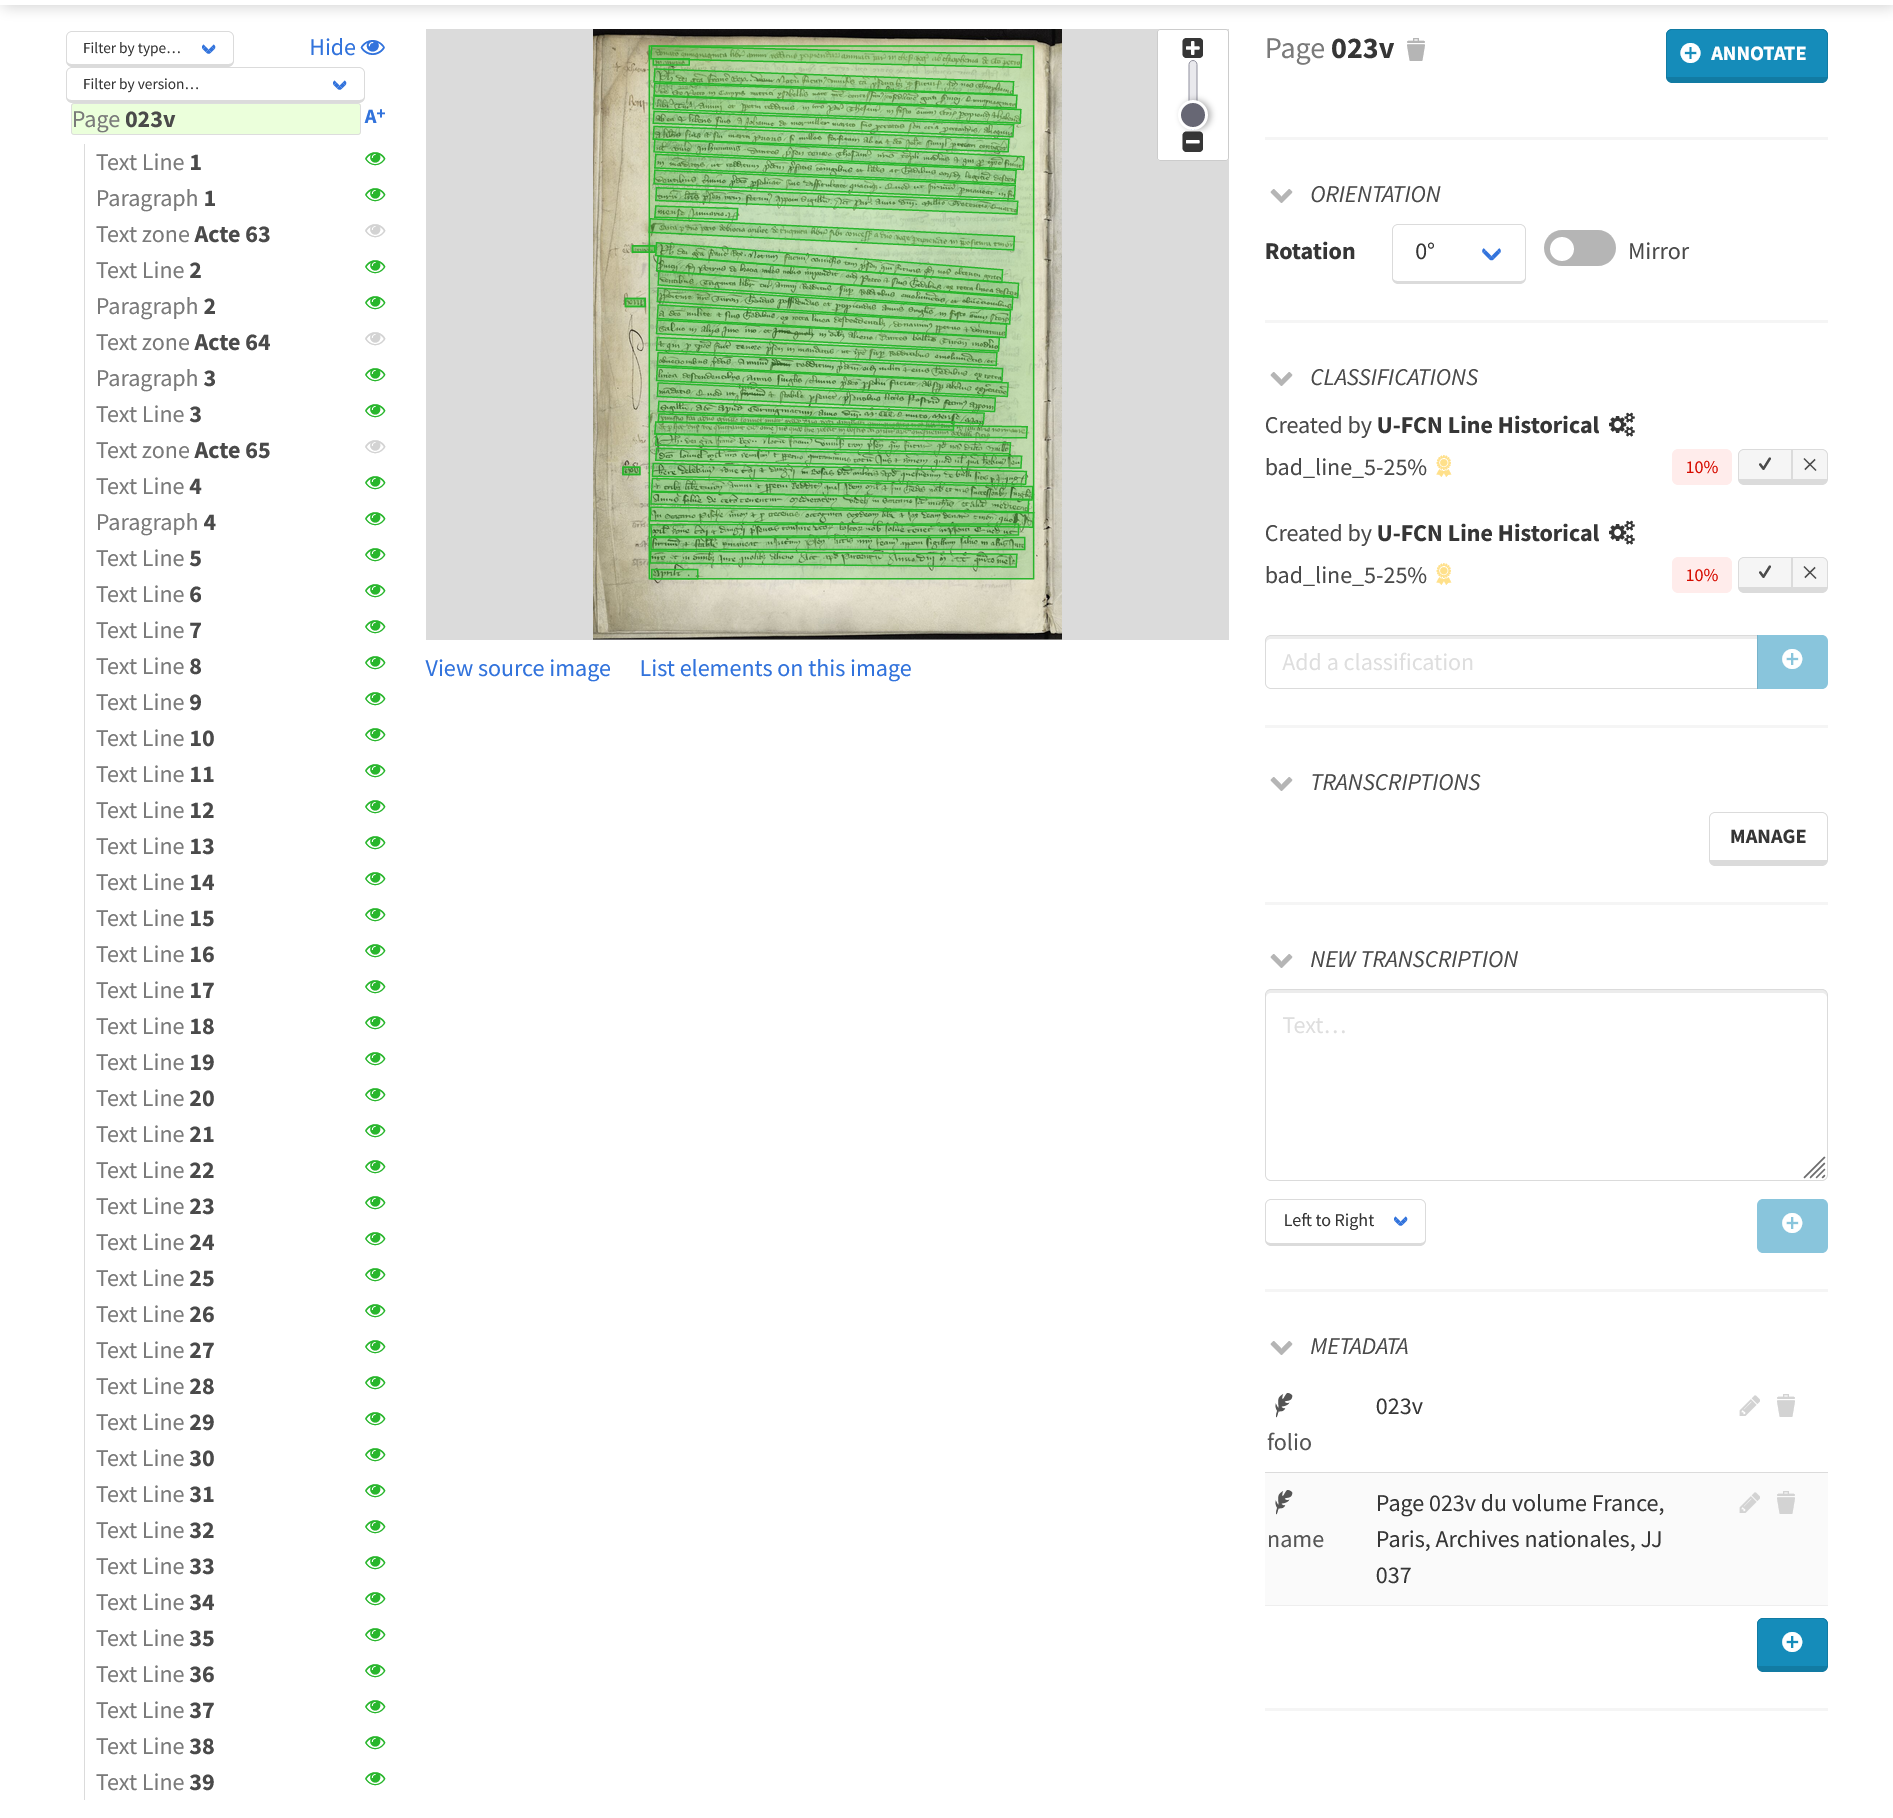
\includegraphics[width=\textwidth]{Images/Interface_Arkindex.png}
		\caption{Segmentation initiale des pages dans la plateforme Arkindex. L'élément page comprend à gauche les éléments enfants, au centre l'image de la page avec les éléments \og Paragraph\fg{} et \og Text Line\fg{} en surbrillance et à droite les métadonnées associées à la page.}
		\label{Page_Initiale_Arkindex}
	\end{figure}
	
	
	\subsection{Des zones de texte comme interface entre actes et pages}
	
	Le texte est ici segmenté en fonction de sa structure physique par des éléments qui découlent directement des éléments pages. Or cette méthode ne permet pas d'associer directement le résultat au contenu des registres. En effet les descriptions disponibles concernent essentiellement la structure logique des textes. Pour faire le lien entre un acte et les éléments qui le concernent dans l'inventaire, il faut donc transformer la segmentation des zones de texte en fonction de la structure logique. En effet, cette dernière ne correspond pas toujours à la structure physique : il est fréquent qu'une page contienne plusieurs actes ou qu'un acte soit présent dans plusieurs pages. Il arrive même que les pages portant les parties d'un même acte ne soient pas à la suite les unes des autres et que d'autres actes entrecoupent ces parties.
	
	La segmentation du contenu des registres a donc été revue pour être organisée en fonction des actes qu'ils contiennent et non en fonction des pages. Il a donc été imaginé un niveau supplémentaire de segmentation au travers des zones de textes. Celles-ci correspondent aux différents composants d'un acte au sein des pages. Ils sont donc à la fois une composante des actes et des pages et forment une interface entre la structure physique et la structure logique des registres.
	
	\section{Des métadonnées prêtes à l’import}
	
	\subsection{Alignement des données issues d'Arkindex et des inventaires}
	
	Les inventaires des registres du Trésor des chartes\footnote{\cite{glenisson_registres_1958}. Pour une description plus précise du contenu des instruments de recherche, \textit{cf}. chapitre 3.} ont donc été utilisés pour extraire les différentes données permettant de décrire ces actes et les aligner avec celles issues de la plateforme Arkindex. Le tout a été organisé sous la forme d'un fichier JSON au sein duquel les actes ont été ordonnés par volume puis par son rang au sein du volume.
	
	\begin{figure}
		\centering
		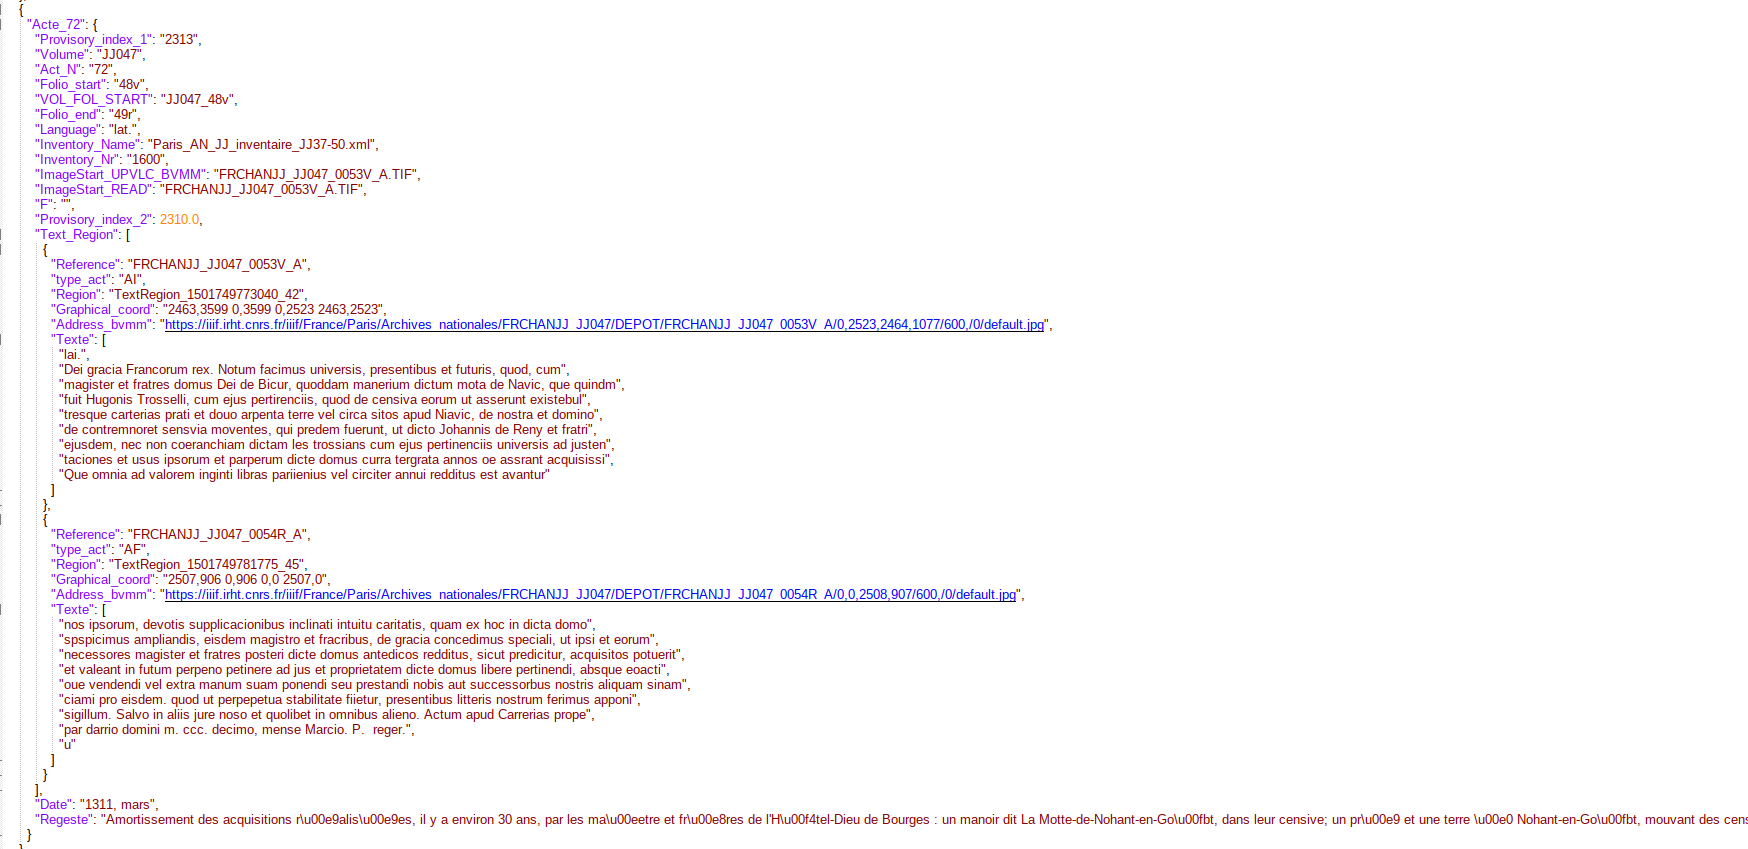
\includegraphics[width=\textwidth]{Images/json_zones_textes.png}
		\caption{Exemple d'un acte contenu par le fichier JSON sous sa forme initiale.}
		\label{json_initial}
	\end{figure}
	
	Les actes se présentent sous la forme d'un élément dictionnaire (\textit{cf}. figure \ref{json_initial}) dont les clefs sont le numéro du volume, le numéro de l'acte dans le volume, le folio de début de l'acte, le folio de fin de l'acte, la langue, la référence de l'inventaire, le numéro de l'acte dans cet inventaire, le nom de l'image dans la BVMM, la date, la description de l'acte par l'inventaire et plusieurs numérotations provisoires utilisées au cours de ce travail. Une dernière clef contient sous forme d'une liste de dictionnaires l'ensemble des données sur les zones de texte qui forment ces actes. Ces données sont issues de la segmentation en acte de la transcription automatique des images des manuscrits\footnote{Il s'agit ici d'une transcription inédite réalisée à l'aide du logiciel Transkribus.}. Chaque zone de texte est composée de la transcription ligne à ligne, de la référence de l'image, des coordonnées de la zone dans l'image, de l'url correspondant à ces coordonnées et de la partie de l'acte que représente cette zone. Cette dernière métadonnée peut prendre plusieurs formes : \og AC\fg{} pour les actes composés d'une seule zone de texte, \og AI\fg{}, \og AM\fg{} et \og AF\fg{} pour les actes composés de plusieurs zones de textes successives ou \og AS\fg{} pour les zones de textes qui ne sont pas à la suite des zones précédentes.
	
	\subsection{Normalisation des éléments}
	
	Afin d'envisager l'import de toutes ces données au sein d'Arkindex\footnote{Nous décrirons plus précisément ce travail au chapitre 8.}, nous avons été confrontés au problème de la normalisation des données. Par exemple, les dates peuvent se présenter sous différentes formes :
	
	\begin{quotation}
		\textquotesingle Date\textquotesingle : \textquotesingle 1317, 16 février\textquotesingle 
	\end{quotation}
	
	\begin{quotation}
		\textquotesingle Date\textquotesingle : \textquotesingle 10 janvier 1359\textquotesingle
	\end{quotation}

	\begin{quotation}
		\textquotesingle Date\textquotesingle : \textquotesingle 1304-1305\textquotesingle
	\end{quotation}
	
	\noindent Nous avons donc écrit un script python contenant un arbre de décision pour transformer ces dates en fonction de la manière dont elles se présentent\footnote{	\url{https://github.com/virgile-reignier/Memoire-TNAH-2022-Reignier/blob/main/Scripts/Normalize_json/normalize_date.py}.}. Une fois normalisée, la date prend la forme d'une liste contenant soit un élément dictionnaire unique dans le cas d'une date précise :

	\begin{quotation}
		\textquotesingle Date-normalisee\textquotesingle: [\\
		\indent\indent\{\\
		\indent\indent	\textquotesingle type\textquotesingle: \textquotesingle when\textquotesingle,\\
		\indent\indent	\textquotesingle year\textquotesingle: 1359,\\
		\indent\indent	\textquotesingle month\textquotesingle : 1,\\
		\indent\indent	\textquotesingle day\textquotesingle : 10\\
		\indent\indent\}\\
		\indent ]\\
	\end{quotation}

	\pagebreak
	
	\noindent soit deux éléments dans le cas d'un intervalle :
	
	\begin{quotation}
				\textquotesingle Date-normalisee\textquotesingle : [\\
				\indent\indent		\{ \\
				\indent\indent		\textquotesingle type\textquotesingle : \textquotesingle notBefore\textquotesingle \\
				\indent\indent		\textquotesingle year\textquotesingle : 1304,\\
				\indent\indent		\textquotesingle month\textquotesingle : null,\\
				\indent\indent		\textquotesingle day\textquotesingle : null\\
				\indent\indent	\},\\
				\indent\indent	\{\\
				\indent\indent		\textquotesingle type\textquotesingle : \textquotesingle notAfter\textquotesingle ,\\
				\indent\indent		\textquotesingle year\textquotesingle : 1305,\\
				\indent\indent		\textquotesingle month\textquotesingle : null,\\
				\indent\indent		\textquotesingle day\textquotesingle : null\\
				\indent\indent	\}\\
				\indent	]\\
	\end{quotation}
	
	\noindent Un certain nombre de formes uniques ont également été repérées au cours de cette étape puis normalisées manuellement, comme par exemple :
	
	\begin{quotation}
		\textquotesingle Date\textquotesingle : \textquotesingle 1323, 3 septembre (corriger 13 septembre ?)\textquotesingle
	\end{quotation}

	\noindent La normalisation des langues a suivi un processus similaire car elles se présentaient initialement sous plusieurs formes :
	
	\begin{quotation}
		\textquotesingle Language\textquotesingle : \textquotesingle lat. et fr.\textquotesingle
	\end{quotation}

	\begin{quotation}
		\textquotesingle Language\textquotesingle : \textquotesingle francais\textquotesingle
	\end{quotation}
	
	\pagebreak
	
	\noindent Nous avons ici aussi rédigé un script python pour normaliser ces données sous une forme unique\footnote{\url{https://github.com/virgile-reignier/Memoire-TNAH-2022-Reignier/blob/main/Scripts/Normalize_json/normalize_language.py}.}. Le résultat se présente donc sous la forme d'un élément dictionnaire contenant la norme utilisée\footnote{Pour la liste des codes décrits par la norme iso-639-3, \textit{cf}. \url{https://fr.wikipedia.org/wiki/Liste_des_codes_ISO_639-2}.} et la liste des langues reconnues encodées en fonction de cette norme :
	
	\begin{quotation}
				\textquotesingle normalized\_language\textquotesingle : \{\\
			\indent\indent \textquotesingle norme\textquotesingle : \textquotesingle iso-639-3\textquotesingle ,\\
			\indent\indent \textquotesingle language\textquotesingle : [\\
			\indent\indent\indent \textquotesingle lat\textquotesingle ,\\
			\indent\indent\indent \textquotesingle frm\textquotesingle \\
			\indent\indent]\\
			\indent\}
	\end{quotation}
	
	\noindent La dernière étape de ce travail consistait à revoir les numérotations provisoires établies précédemment. Le contenu du fichier a en effet été modifié au cours du temps, ce qui a affecté leur forme. L'attribut \og provisory\_index\_2\fg{} s'est ainsi trouvé avec une valeur vide à plusieurs reprises. Au contraire, des valeurs \og bis\fg{} ont été ajoutées à l'attribut \og provisory\_index\_1\fg{} qui n'est donc pas complètement linéaire :
	
	\begin{quotation}
		\textquotesingle Provisory\_index\_1\textquotesingle : \textquotesingle 8774\textquotesingle
	\end{quotation}
	
	\begin{quotation}
		\textquotesingle Provisory\_index\_1\textquotesingle : \textquotesingle 8774bis\textquotesingle
	\end{quotation}

	\begin{quotation}
		\textquotesingle Provisory\_index\_1\textquotesingle : \textquotesingle 8775\textquotesingle
	\end{quotation}
	
	\noindent Nous avons donc créé un nouvel attribut \og Provisory\_index\_3\fg{} permettant d'associer chaque acte à un entier unique correspondant à son rang dans le fichier :
	
	\begin{quotation}
		\textquotesingle Provisory\_index\_3\textquotesingle : 8774
	\end{quotation}

	\begin{quotation}
		\textquotesingle Provisory\_index\_3\textquotesingle : 8775
	\end{quotation}
	
	\begin{quotation}
		\textquotesingle Provisory\_index\_3\textquotesingle : 8776
	\end{quotation}

	\begin{figure}
		\centering
		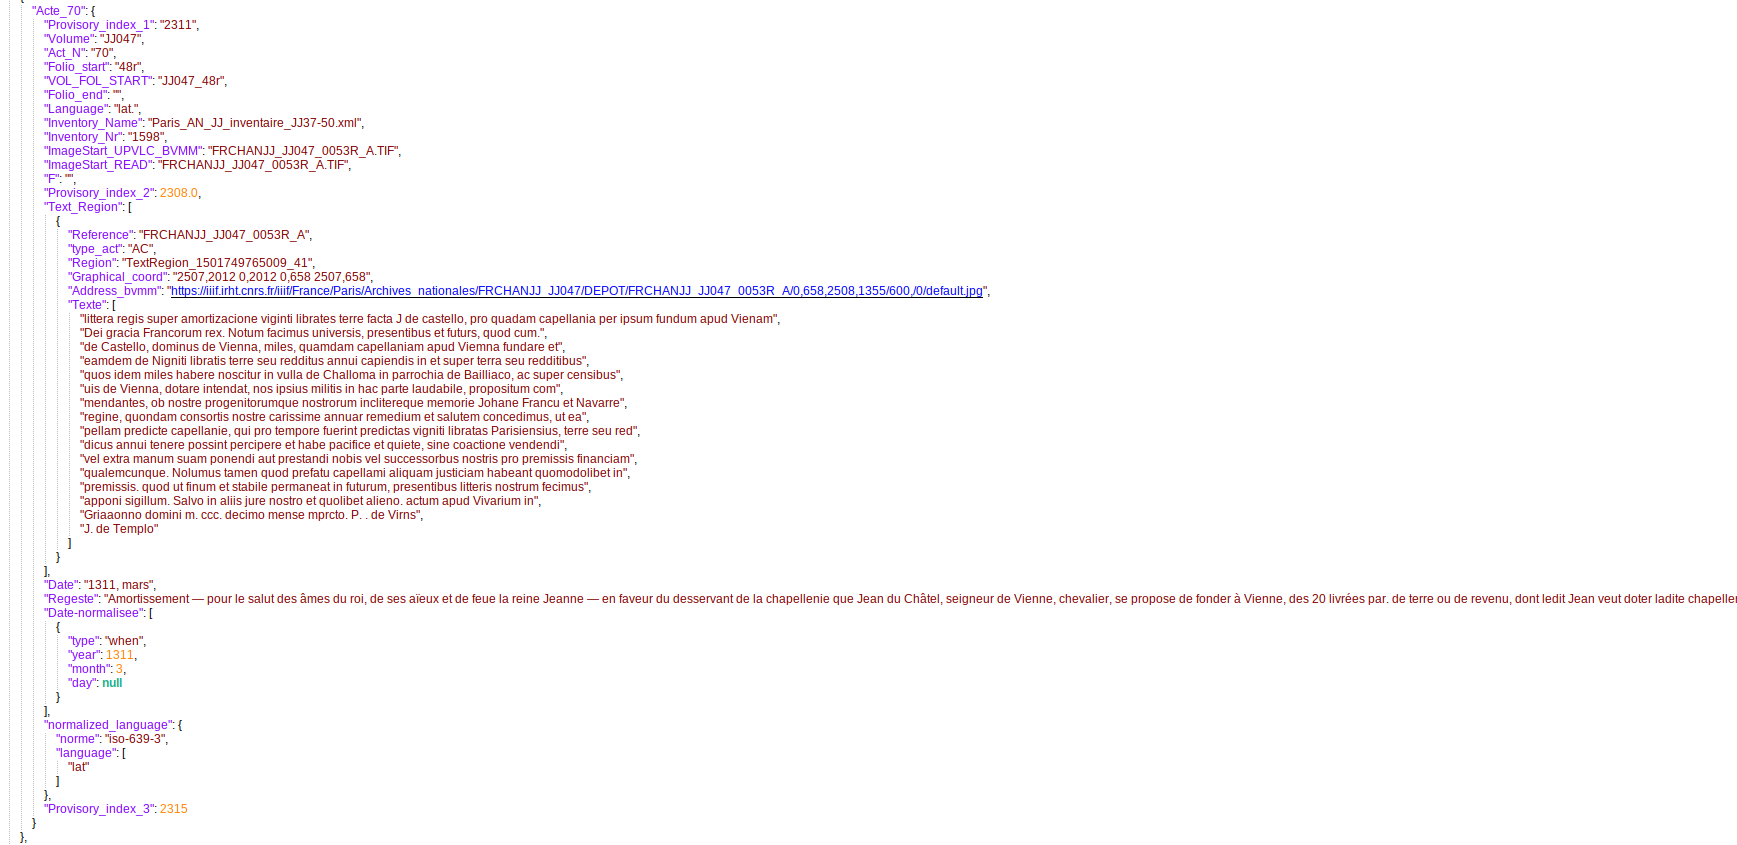
\includegraphics[width=\textwidth]{Images/json_modifie.png}
		\caption{Exemple d'un acte contenu par le fichier JSON après normalisation des éléments}
		\label{json_final}
	\end{figure}
	
	
	\section*{Conclusion}
	
	Ce chapitre nous a permis d'aborder les différents éléments disponibles grâce aux recherches réalisées au sein du projet Himanis et dans les opérations qui lui ont succédés. Ces recherches ont abouti au développement de modèles de REM et de REN applicables aux textes médiévaux. Par la suite, ces travaux ont permis de proposer une transcription automatique des registres du Trésor des chartes et un travail de transformation a été réalisé pour associer la structure physique à la structure logique des textes et permettre un alignement de cette transcription avec les données présentes dans les inventaires. Après quelques modifications réalisées pendant le stage, nous disposons maintenant d'un fichier complet décrivant l'ensemble du contenu des registres JJ 35 à JJ 91. La figure \ref{json_final} présente un exemple du format final des actes décris dans ce fichier.
	
	
	\chapter{\textit{Legacy Metadata} : numérisation et exploitation des instruments de recherche}
	
	Comme nous l'avons vu, les travaux réalisés à partir du projet Himanis se sont appuyés à plusieurs reprises sur les instruments de recherche qui concernent le Trésor des chartes, que ce soit pour la construction du modèle de REM à partir des éditions de Paul Guérin ou pour la description du contenu des registres à partir des inventaires systématiques. Ces ouvrages contiennent en effet tout un ensemble de données disponibles pour appréhender le contenu des registres. Conçus selon une structure logique facilement identifiable, ces outils de travail forment une masse de \textit{legacy data} permettant d'associer chaque élément de la structure logique à toute une série de méta-données. Leur traitement numérique prend donc toute sa place dans le cadre de la recherche sur la lecture automatique des registres et compose à ce titre le principal matériel sur lequel s'est appuyé notre travail de stage.
	
	Ce chapitre sera consacré à l'utilisation des instruments de recherche du Trésor des chartes dans le cadre des travaux initiés par le projet Himanis. Nous présenterons dans un premier temps les différents outils disponibles et leurs lacunes. Puis nous exposerons les transformations réalisées à partir de ces ouvrages afin de structurer leur contenu sous format numérique. Pour finir, nous décrirons le projet de structuration de l'index dans lequel notre stage s'est inséré.
	
	\section{Description du matériel disponible}
	
	\subsection{Inventaires systématiques et géographiques}
	
	Corpus incontournable pour étudier le pouvoir des rois de France à la fin du Moyen Âge, le Trésor des chartes a été l'objet de nombreuses études qui ont permis d'en diffuser largement le contenu. Ces travaux ont été complétés par plusieurs projets archivistique de description systématique des registres pour faciliter l'accès au contenu de ce fonds\footcite{stutzmann_recherche_2017}. L'outil le plus complet et le plus précis est l'inventaire analytique des registres du Trésor des chartes publié par les Archives Nationales entre 1958 et 1999\footcite{glenisson_registres_1958}. Il propose une analyse systématique des actes contenus dans les registres JJ 37 à JJ 79B avec le rang de l'acte dans l'inventaire, les dates de temps et de lieu, un résumé de l'acte, le numéro de l'acte dans le volume, le folio de début (et parfois de fin) et de potentiels renvois (\textit{cf}. figure \ref{inventaire_papier}).
	
	\begin{figure}
		\centering
		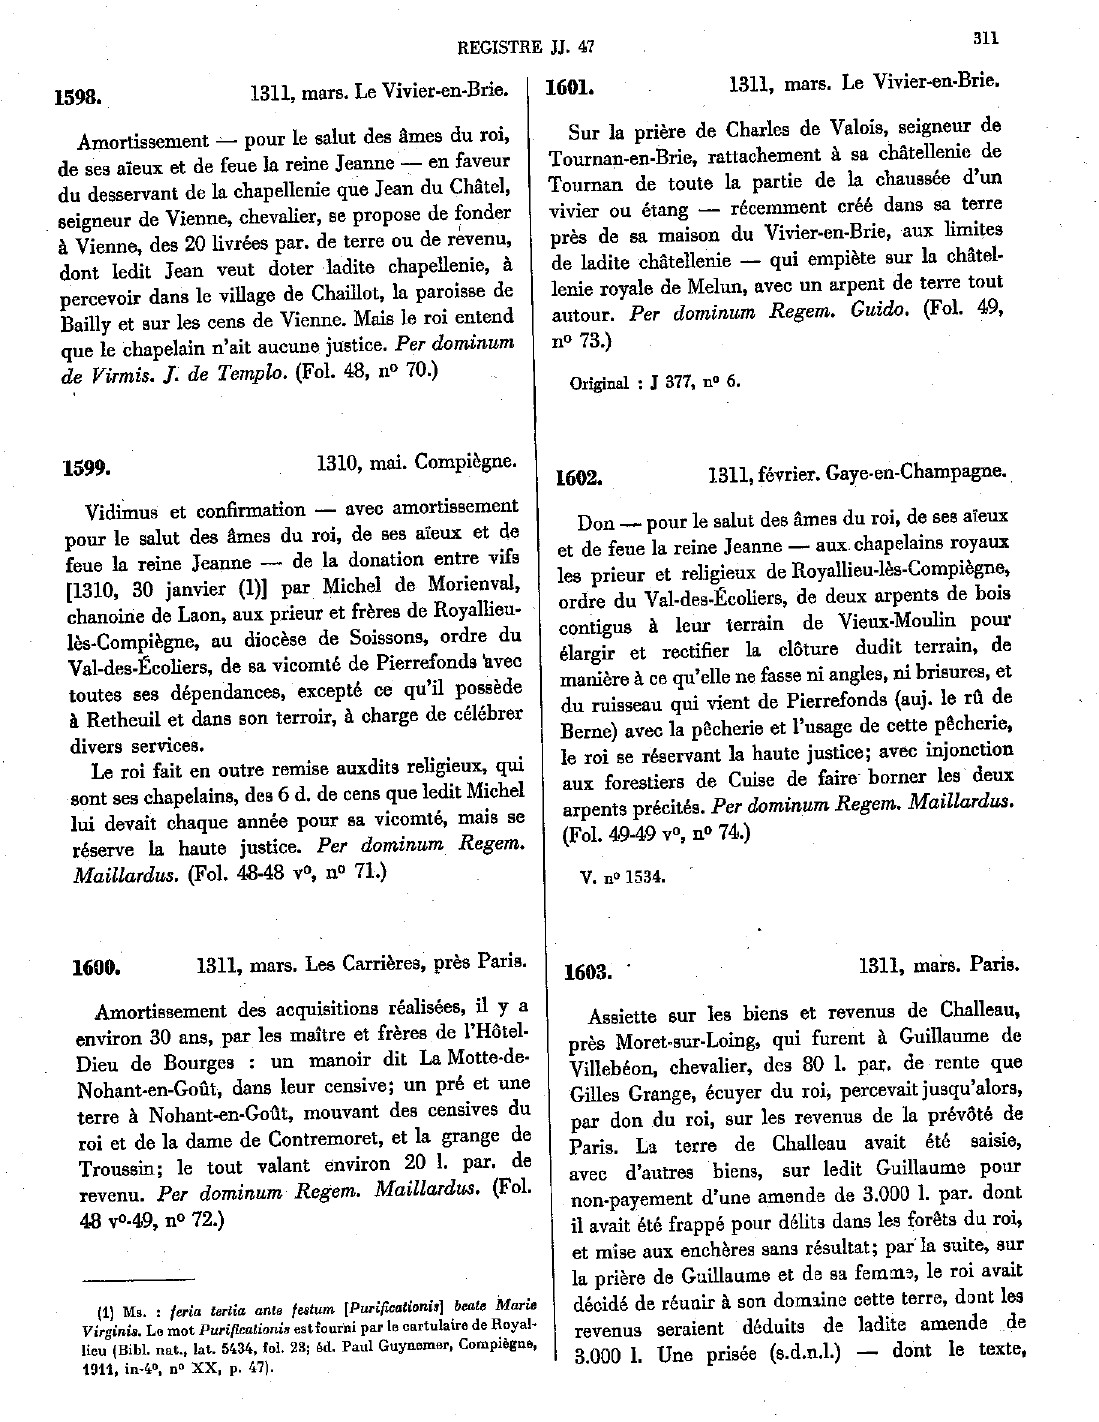
\includegraphics[width=\textwidth]{Images/Inventaire_papier.jpg}
		\caption{Exemple d'analyses contenues dans l'inventaire des registres du Trésor des chartes publié sous la dir. de Robert Fawtier.}
		\label{inventaire_papier}
	\end{figure}
	
	Ces ouvrages disposent également d'une suite sous forme manuscrite ou dactylographiée pour les registres JJ 80 à JJ 98 réalisée par Y. Lanhers, A. Vallée, S. Clémencet et P. Luc entre 1945 et 1985\footnote{Archives Nationales, IR 49 à IR 59, IR 5127 et IR 50000.}. Le travail d'inventaire systématique ne recouvre cependant pas l'ensemble du corpus et les seuls instruments disponibles pour les registres de la fin du Moyen Âge sont les inventaires thématiques qui recensent systématiquement les actes selon un axe précis. Les plus complets sont trois inventaires géographiques rassemblant les actes qui concernent la Gascogne, le Languedoc, le Rouergue et la Loire Moyenne\footcite{samaran_gascogne_1966, dossat_languedoc_1983, chevalier_les_1993}.
	
	\subsection{Documentation complémentaire : inventaires papier, éditions et indexations}
	
	Un autre moyen de compléter ces lacunes est d'utiliser les instruments de recherche anciens dressés au XVIII\ieme\ siècle et complétés au XIX\ieme. Leur niveau de détail est cependant assez faible puisqu'ils se contentent de compiler les tables des actes contenues dans les registres\footnote{Inv. ms. de JJ 1 à JJ 264, dressé au début du XVIIIe s., révisé et complété par A. Longnon et A. Coulon, 1880-1900, copie en quatre vol., IR421-IR424 et IR 429 ; Acta omissa. Inv. somm. ms. de la série JJ, actes non mentionnés dans	l’inv. de A. Longnon et A. Coulon, 1898-1900, IR33-IR34.}. On retrouve également des informations précieuses dans les éditions partielles des actes du Trésor des chartes. Outre celle de Guérin citée plus haut, il en existe 4 autres consacrées à Amiens, Paris pendant le règne de Philippe VI et la Normandie et Paris pendant l'occupation anglaise au début du XV\ieme\ siècle\footcite{guerin_actes_1881, viard_documents_1899, longnon_paris_1878, le_cacheux_actes_1907, maugis_documents_1908}. Un autre moyen d'accéder au contenu des registres est d'utiliser un index des sujets, noms de personnes et noms de lieux. La plupart des ouvrages que nous venons de citer en contiennent, à l'exception notable du tome II de l'inventaire analytique des registres du Trésor des chartes pour lequel un index des noms de lieux est en préparation. Enfin, deux instruments permettent d'aborder les actes des registres à partir des noms de lieux, personnes et sujets pour les registres de Charles VI et Henri VI\footnote{Archives Nationales, IR 1810 et Projet d'inventaire par C. Gut, 2010.}. Ils sont disponibles respectivement sous forme de fiches papiers et d'un fichier texte. 
	
	Ainsi donc, le matériel disponible pour étudier ce corpus est à la fois conséquent et très lacunaire. Alors que des pans entiers sont connus de manière précise grâce aux inventaires systématiques et géographiques, un grand nombre de registres ne disposent que d'instruments très primaires pour repérer le contenu qui intéresse le chercheur et éviter un dépouillement systématique de ces archives. L'automatisation de l'analyse archivistique est donc un enjeu essentiel car elle permet de rendre accessible la lecture des registres et d'envisager leur dépouillement ponctuel et précis. Cet accès facilite ainsi la recherche sur certains sujets comme par exemple l'étude du pouvoir du roi de France.  

	\section{Formats de l’information}
	
	\subsection{Segmentation en XML}
	
	Un certain nombre des outils que nous avons décrits ont déjà été numérisés et convertis par les Archives Nationales sous format EAD, une norme utilisant le langage XML pour structurer des descriptions de manuscrits ou de documents d’archives. Ils présentent cependant quelques variations dans leur format, c'est pourquoi les membres du projet Himanis ont fait ici le choix de tout transformer sous un format homogène utilisant la norme TEI, un autre format basé sur le langage XML. L'objectif est de pouvoir combiner les transcriptions des textes avec les métadonnées les concernant\footcite{stutzmann_recherche_2017}.
	
	\begin{figure}
		\centering
		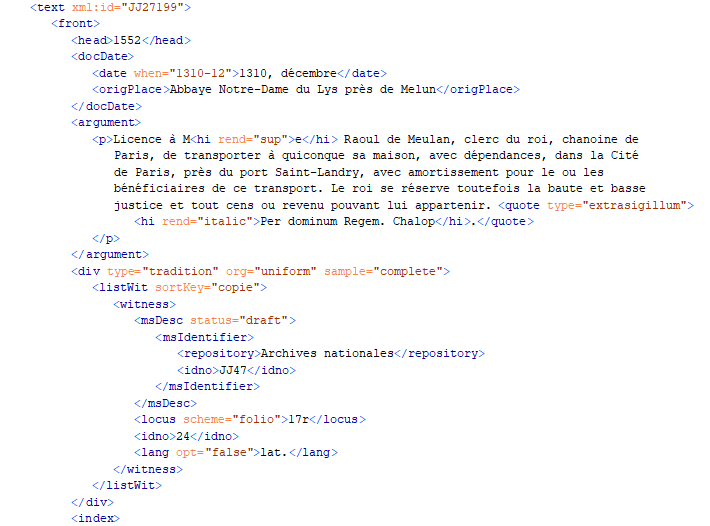
\includegraphics[width=\textwidth]{Images/Inventaire_en_TEI.png}
		\caption{Exemple d'analyse d'un acte du Trésor des chartes encodée sous format XML-TEI.}
		\label{inventaire_TEI}
	\end{figure} 
	
	Comme présenté par la figure \ref{inventaire_TEI}, chaque acte y est encodé au sein d'un élément <text> disposant d'un attribut @xml:id permettant de lui associer un identifiant unique. Les balises enfants contiennent ensuite le rang de l'acte dans l'inventaire, les dates de lieu et de temps, l'analyse du texte et sa manifestation physique dans les registres du Trésor des chartes. Les fichiers ont par la suite été mis en ligne dans le répertoire Github du projet\footnote{\url{https://github.com/oriflamms/himanis/tree/master/Inventories}.} et leur contenu a servi à la constitution d'un fichier sous format JSON décrivant les actes des registres inventoriés\footnote{\textit{Cf}. chapitre 2.}.
	
	\subsection{Numérisation de l’index}

	Ce travail de segmentation du contenu des instruments de recherche pour l'organiser sous le format XML-TEI a également été réalisé pour les différents index qui accompagnent ces ouvrages. Chaque entrée est insérée dans une balise <p> qui peut contenir une ou plusieurs balises <seg> en fonction du nombre de sous-entrées présentes. L'entité et sa description sont ensuite insérées dans une balise <term> et les renvois vers les actes décrits par l'index sont rassemblés dans une balise <num>. Chaque renvoi est ensuite inséré dans une balise <idno> (\textit{cf}. figure \ref{index_TEI}).
	
	\begin{figure}
		\centering
		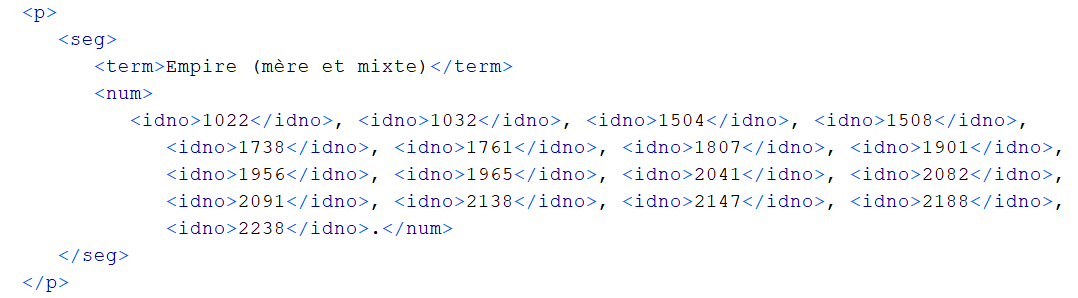
\includegraphics[width=\textwidth]{Images/index_en_TEI.png}
		\caption{Exemple d'une entrée d'index encodée sous format XML-TEI.}
		\label{index_TEI}
	\end{figure} 
	
	Une des difficultés de ce travail a été de reconstituer les sous-entrées de l'index. Le corps de certaines est en effet directement dépendant de celui de l'entrée principale, ce qui rend délicat sa manipulation comme une entité isolée. Par exemple l'entrée :
	
	\begin{quotation}
		Récupérations : des arrérages de bois
	\end{quotation}

	\noindent est suivie de la sous-entrée :
	
	\begin{quotation}
		des droits royaux
	\end{quotation}

	\noindent Cette dernière n'a pas de sens prise isolément, il faut donc ici reconstituer la notion dans son ensemble : \og Récupérations des droits royaux\fg{}. Ce travail de reconstitution a été réalisé en s'appuyant autant que possible sur la structure de l'index : les \og :\fg{} servent ici de séparateur entre l'entrée principale et les sous-entrées, tandis que ces dernières sont systématiquement séparées par un \og ; — \fg{}. Le travail réalisé a donc consisté à éliminer le premier séparateur et à transformer le second en \og{}  , — \fg{} afin de bien marquer les entrées dont le corps dépend de celui d'une entrée générale. Pour les cas exposés, la segmentation en TEI donne le résultat suivant :
	
	\begin{quotation}
		<term>Récupérations des arrérages de bois</term>
	\end{quotation}

	\begin{quotation}
		<term>Récupérations , — des droits royaux</term>
	\end{quotation}

	\section{Les index comme compléments aux métadonnées décrivant les actes ?}

	\subsection{Le projet : mettre à plat les entrées d’index}
	
	L'objectif de ce travail était ainsi de faciliter l'association de chaque entrée d'index aux entrées d'inventaire qui lui correspondent. En effet, le but du processus était d'utiliser cet index comme vérité terrain pour développer l'apprentissage du liage d'entités. L'index a donc été mis à plat en fonction de cette logique : toutes les balises <idno> dans les entrées d'index ont été utilisées pour identifier l'entrée d'inventaire contenant la notion décrite par cette entrée. Afin que le lien soit bien manifeste, les entrées d'inventaires décrites en TEI ont été enrichies d'une balise <index> contenant l'ensemble des entrées d'index renvoyant vers l'acte en question. La figure \ref{index_in_inventaire} donne un exemple de ces entrées d'index encapsulées dans des éléments <term> et disposant d'un attribut @type dont la valeur est \og place\fg{}, \og person\fg{} ou \og subject\fg{} en fonction du type d'entrée dont il s'agit\footnote{A propos de la typologie des entrées, \textit{cf}. chapitre 4.}.
	
	\begin{figure}
		\centering
		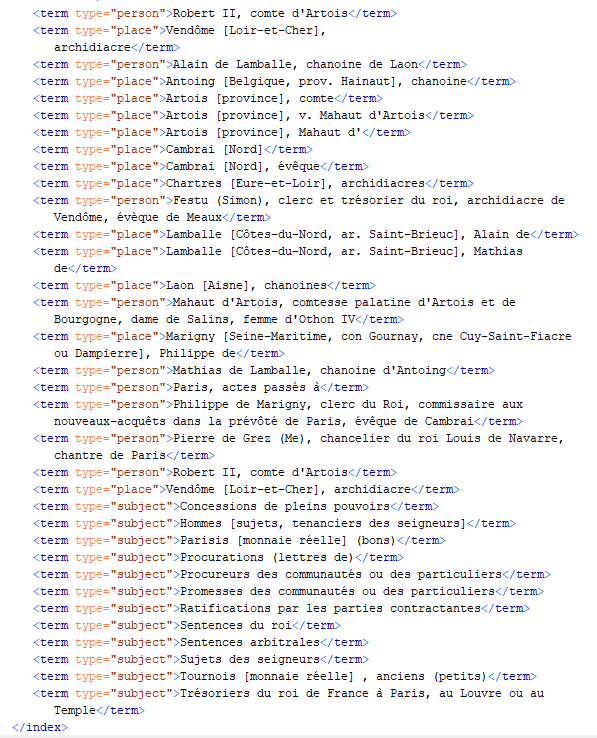
\includegraphics[width=\textwidth]{Images/Index_in_inventaire.png}
		\caption{Exemple d'une liste d'entrées d'index contenue dans une balise <index> insérée dans l'entrée d'inventaire sous format XML-TEI qui lui correspond.}
		\label{index_in_inventaire}
	\end{figure}
	
	Le projet était d'inscrire directement les entrées d'index au sein des métadonnées de l'acte afin qu'elles puissent être comprises comme autant d'entités nommées contenues dans le texte. Cela devait faciliter l'association entre texte et entités nommées et façonner la vérité terrain permettant l'apprentissage du liage d'entités. Cette vision de l'index mis à plat comme une extension de l'inventaire jointe aux métadonnées des actes a largement guidé la segmentation des entrées car il fallait que chacune se suffise à elle-même pour qu'on puisse la comprendre comme une entité nommée à reconnaître.
	
	\subsection{Perte de qualité et de complexité dans les données}
	
	Cette vision des choses n'est cependant pas sans poser quelques problèmes dans la mise en œuvre du liage d'entités. L'index ainsi mis à plat correspond en effet moins à une base de connaissances proprement dite qu'à un ensemble d'entités nommées associées au texte. Elle ne permet pas l'apprentissage du liage puisqu'elle ne se fonde pas sur un référentiel en tant qu'entité autonome du texte. Les entités nommées sont ici simplement répétées au lieu où elles ont été reconnues et ne disposent pas de métadonnées pour les décrire (définition du concept, synonymes, coordonnées géographiques, ...). L'absence de référentiel unique et autonome ne permet donc pas le traitement \textit{a posteriori} des entrées pour les segmenter en différentes parties ou les enrichir par alignement avec d'autres référentiels. C'est ainsi que l'absence d'identifiant unique pour les entrées d'index condamne le travail à rester dans l'état où il est au moment de la mise à plat alors que le liage d'entités peut aussi conduire à augmenter le nombre d'entités nommées identifiées dans les textes.
	
	De plus, l'index se caractérise par un ensemble de relations entre les entrées : associations entre entrées générales et sous-entrées, renvois contenus dans les données, ou encore entrées rejetées vers une autre entrée. Or ces relations, qui ne peuvent être reportées par la mise à plat de l'index, sont essentielles à plusieurs titres pour construire le travail de liage d'entités.  Par exemple, les entrées rejetées ne contenant pas de renvois vers l'inventaire mais uniquement un renvoi vers une autre entrée d'index sont complètement invisibilisées lors de ce travail de mise à plat alors qu'elles fournissent autant d'alias d'une même notion mobilisables au moment de la construction de la base de connaissances. De même les renvois contenus dans les entrées et les relations entre entrées générales et sous-entrées permettent d'appréhender l'association entre les entités et les possibles synonymies ou co-occurences de celles-ci, elles sont donc nécessaires à la bonne réalisation du liage. Il apparaît donc que l'utilisation de l'index comme un ensemble de métadonnées associées aux actes ne fournit pas un cadre optimal à la mise en œuvre du liage d'entités. La bonne compréhension du projet initial en vue duquel les données ont été manipulées est cependant essentielle pour saisir l'enjeu des étapes déjà réalisées et aborder celles que nous avons menées pour tenter d'avancer dans une direction plus propice à la constitution d'un référentiel.
	
	\section*{Conclusion}
	
	Nous avons vu que le Trésor des chartes dispose d'un certain nombre d'instruments de recherche. Ces ouvrages sont une mine d'information pour développer la lecture automatique des textes puisqu'ils fournissent un grand nombre de métadonnées décrivant le contenu des registres. Les membres du projet Himanis ont donc travaillé à leur numérisation et leur segmentation pour les inclure dans un modèle sous format XML-TEI. Cette transformation a placé l'acte comme élément central de description du corpus, chacun d'entre eux étant associé à l'ensemble des métadonnées disponibles pour le décrire. Ce travail a cependant trouvé sa limite au moment de la mise à plat de l'index comme devant accompagner l'ensemble de métadonnées. Les entrées d'index ne peuvent en effet pas se réduire à un ensemble d'entités nommées reconnues dans un texte et doivent constituer un référentiel propre afin de modéliser la complexité de leur définition et de leurs relations entre elles et avec les textes, puis assurer l'apprentissage du liage d'entités à partir de données d'entraînement. Nous avons donc consacré un temps conséquent du stage à travailler sur ces entrées d'index pour comprendre leur complexité et la meilleure manière de la prendre en compte pour leur utilisation future. Dans sa finalité, le projet serait de permettre de compléter les lacunes de ces instruments par l'indexation automatique des registres dont le contenu n'a pas été décrit de manière systématique.
	
	\chapter*{Conclusion partielle}
	
	Cette première partie nous a permis d'exposer dans son ensemble le contexte de travail dans lequel nous avons réalisé notre stage. Notre développement a commencé par un premier chapitre consacré à l'état de l'art sur le liage d'entités et son utilisation dans l'étude des documents patrimoniaux. Ensuite, nous avons dédié un second chapitre à la description des différents travaux réalisés au sein du projet Himanis ou à sa suite et des résultats disponibles pour poursuivre les recherches sur le liage d'entités. Nous avons enfin terminé cet exposé par un troisième chapitre portant sur l'utilisation des instruments de recherche disponibles comme \textit{legacy metadata} permettant de décrire le contenu des registres ainsi que les limites de cette logique.
	
	Tout cela nous a permis de voir à quel point le corpus traité par le projet Himanis fournit un terreau favorable au développement du liage d'entités. Cette technique est en effet difficile à mettre ne œuvre pour des documents anciens car elle nécessite une base de connaissances dédiée. Or les instruments de recherches déjà numérisées par les acteurs du projet Himanis facilitent largement la constitution de cette base de connaissances. Les index disponibles se prêtent à la constitution d'un référentiel vers lequel pointer au moment de la réalisation du liage. En plus de fournir un matériel idéal pour l'entraînement d'un modèle, le Trésor des chartes dispose également de tout un ensemble de textes non-indexés qui se prêtent à la mise en œuvre et à l'évaluation de ce modèle.
	
	\parttext{L'objectif final du stage que nous avons réalisé étant de préparer l'apprentissage du liage d'entités à partir des données issues du projet Himanis, notre action s'est principalement concentrée sur la création d'un référentiel pouvant servir de base de connaissances. Nous consacrerons donc cette deuxième partie au travail de modélisation et de formalisation de ce référentiel à partir d'un index papier, activité qui a occupé la majeure partie de notre stage. Nous nous sommes concentrés ici sur l'index du premier volume de l'inventaire analytique des registres du Trésor des chartes portant sur les registres JJ 37 à JJ 50 et paru en 1958. Pour rendre compte de ce travail, nous décrirons dans un premier chapitre les différentes difficultés rencontrées pour comprendre et manipuler cet instrument de recherche. Puis nous dédierons un second chapitre à l'analyse des relations entre les entités. Nous consacrerons enfin un troisième chapitre à la transformation de l'index en une base de données relationnelle.}
	
	\part{Modéliser et formaliser un référentiel à partir d’un instrument de recherche papier}
	
	
	\chapter{Appréhender les \textit{legacy data}}
	
	La mobilisation d'un instrument de travail papier pour construire un référentiel numérique implique de prendre le temps de comprendre les données qu'on utilise. Leur structuration peut en effet suivre une logique complexe, passant de l'utilisation de caractères séparateurs à un grand nombre de renvois implicites. Or cette utilisation n'est pas toujours systématique et la quête de la perfection peut parfois demander un temps de relecture très conséquent pour repérer toutes les erreurs et incohérences qui peuvent se glisser dans les données de manière plus ou moins systématique. Dans le cadre de ce travail, l'index que nous avons manipulé est un ouvrage imprimé qui a été numérisé, transcrit par OCR et préalablement structuré sous la forme d'un fichier au format XML-TEI. Il nous a donc fallu prendre le temps de saisir le projet qui a guidé les différentes étapes de ce travail\footnote{\textit{Cf}. chapitre 3.} et son influence sur l'état des données. Ce temps est nécessaire pour faire le lien entre le fichier que nous avons manipulé et le contenu intellectuel de l'index que nous voulons reporter dans le référentiel.
	
	Ce chapitre sera donc consacré aux différentes difficultés auxquels nous avons été confrontés dans l'analyse de ces \textit{legacy data} et aux solutions mises en œuvre pour y faire face. Pour cela, nous décrirons dans un premier temps les différents types de contenus présents dans les entrées. Puis nous reporterons les différentes exceptions qu'il nous a fallu traiter pendant notre travail. Enfin, nous nous intéresserons aux différentes erreurs qui ont pu être mises au jour tout au long de cette chaîne de traitement.
	
	\section{Des entrées composées de différents éléments}
	
	\subsection{Reconnaître la typologie}
	
	Au début de notre stage, le fichier contenait 20136 balises <term> correspondant à tous les éléments contenus dans l'index. Ces éléments se répartissent en plusieurs catégories. On retrouve tout d'abord quelques éléments titres qui sont nécessaires à l'organisation de l'index mais qui n'appartiennent pas au contenu :
	
	\begin{quotation}
		<term>INDEX DES MATIÈRES</term>
	\end{quotation}

	\begin{quotation}
		<term>T</term>
	\end{quotation}

	\noindent Nous avons ici profité de l'étape de création d'identifiants uniques pour éliminer ces éléments de la suite du processus\footnote{Nous traiterons plus précisément toutes les étapes associées à la gestion des liens entre les entrées au chapitre 5.}. Nous avons cependant utilisé l'indication offerte par ces titres sur la séparation entre les deux parties de l'index. Celui-ci est en effet constitué d'abord d'un index des matières qui recense tous les sujets mentionnés dans les actes, puis d'un index des noms de personnes et de lieux. 
	
	Cette séparation a servi de base à l'établissement d'une typologie des entrées. Toutes les entrées présentes dans l'index des matières ont été associées au type \og subject\fg{} tandis que les entrées de l'index des noms de personnes et de lieux ont dû être analysées pour discriminer celles qui relèvent du type \og person\fg{} et celles qui relèvent du type \og place\fg{}. Cette étape avait déjà été anticipée avant le début de mon stage à partir d'un principe simple : les entrées disposant de crochets ont été marquées comme des \og place\fg{} et celles n'en disposant pas comme des \og person\fg{}. Cela donne ainsi le résultat suivant : 
	
	\begin{quotation}
		<term type=\textquotesingle place\textquotesingle >Montreuil [Pas-de-Calais]</term>
	\end{quotation}

	\begin{quotation}
		<term type=\textquotesingle person\textquotesingle >Montreuil (Pierre de)</term>
	\end{quotation}

	\noindent Si cette séparation est pertinente dans la plupart des cas, il arrive cependant que cela conduise à un certain nombre d'erreurs :
	
	\begin{quotation}
		<term type=\textquotesingle place\textquotesingle >Dreux (Jean) [à Orléans]</term>
	\end{quotation}
	
	\begin{quotation}
		<term type=\textquotesingle person\textquotesingle >Agulhou (pièce de terre dite), dans le territoire de
			Béziers</term>
	\end{quotation}
	
	\noindent Nous avons donc tenté de repérer les erreurs systématiques qui peuvent exister dans ces données. Pour cela, nous avons notamment cherché toutes les occurrences de \og terre\fg{}, \og bien\fg{}, \og bois\fg{}, \og près\fg{}, ... pour rétablir la valeur de l'attribut @type vers \og place\fg{}. Un autre problème systématique concerne les personnes dont le nom renvoi vers un toponyme :
	
	\begin{quotation}
		<term type=\textquotesingle place\textquotesingle >Aigues-Vives [Lot-et-Garonne, con Monclar, cne Saint-Pastour?]
			(Bérenger d')</term>
	\end{quotation}

	\noindent Nous avons ici fait le choix de considérer ces noms comme relevant du type \og person\fg{}\footnote{Sur les différentes formes de noms de personnes, \textit{cf}. chapitre 5.}. Nous avons utilisé l'expression régulière \og [A-Z].* de$\backslash$)\fg{} (et ses déclinaisons avec \og d'\fg{}, \og des\fg{}, ...) pour les repérer et avons procédé par une méthode semi-automatisée pour les transformer une à une tout en gardant un regard sur la réalisation afin d'éviter les effets de bords pouvant toucher les quelques exceptions de noms de lieu correspondant à ce modèle, comme par exemple :
	
	\begin{quotation}
    	<term type=\textquotesingle place\textquotesingle >Bannes (mas de) [Aveyron, ar. et con Villefranche-de-Rouergue,
			cne Morlhon-le-Haut]</term>
	\end{quotation}
	
	\noindent Les autres erreurs repérées ont été corrigées ponctuellement au fur et à mesure de leur identification au cours de notre travail. Il est possible qu'il en existe encore.
	
	\subsection{Segmentation des entrées}
	
	Une fois ce travail réalisé et l'index mis sous forme d'une table\footnote{Nous décrirons plus précisément cette étape au chapitre 6.}, nous avons pu repérer le contenu des entrées pour en segmenter les différentes parties en fonction du type de données. Nous avons donc rédigé un script python permettant de réaliser cette étape de manière automatisée\footnote{\url{https://github.com/virgile-reignier/Memoire-TNAH-2022-Reignier/blob/main/Scripts/Index/simplification_entrees.py}.}. Les éléments mis entre crochets ont ainsi été ajoutés dans une colonne \og Détails\fg{} et ceux qui sont précédés d'une virgule dans la colonne \og Supplément\fg{}. Cette étape a également permis de construire une colonne \og Entrée\_simplifiée\fg{} construite à partir de l'entrée originelle après extraction des éléments utilisés pour les autres colonnes. L'entrée :
	
	\begin{quotation}
		Chambre aux Deniers, Camera Denariorum [terme encore employé à cette époque pour 	désigner la Chambre des Comptes]
	\end{quotation}

	\noindent a été transformée sous la forme suivante :

	\begin{quotation}
		\begin{tabular}{|p{4cm}|p{4cm}|p{4cm}|}
			\hline
			Entrée\_simplifiée & Détails & Supplément \\ \hline
			Chambre aux Deniers & aux Deniers	terme encore employé à cette époque pour désigner la Chambre des Comptes & Camera Denariorum \\ \hline
		\end{tabular}
	\end{quotation}
	
	\noindent Cette étape a également été accompagnée d'une rationalisation des sous-entrées afin d'éviter la répétition inutile des éléments contenus dans les entrées générales. L'entrée
	
	\begin{quotation}
		Cens cotage [acquitté pour un tènement en roture] , — morts [ne comportant pas de lods et ventes]
	\end{quotation}

	\noindent a ainsi été simplifiée afin que la colonne \og Entrée\_simplifiée\fg{} devienne
	
	\begin{quotation}
		Cens cotage , — morts
	\end{quotation}

	\noindent Les données ainsi segmentées sont disponibles dans le tableau contenant les données de l'index et mis en ligne sur le Github du projet Himanis\footnote{\url{https://github.com/oriflamms/himanis/blob/master/Inventories/Systematic/Paris_AN_JJ_inventaire_JJ37-50_index.xlsx}.}.
	
	\section{Comment utiliser des \textit{semi-structured data} ?}
	
	\subsection{Des cas spécifiques tout au long de la chaîne de traitement}
	
	Le travail d'analyse et de traitement des entrées d'index nous a confronté à quelques difficultés dans l'appréhension des données. Les entrées bénéficient en effet d'une structure sensible et très utile pour comprendre les différents éléments qu'elles contiennent, mais celle-ci n'est jamais pleinement systématique. Nous avons donc fait face à plusieurs surprises tout au long de ce travail. Par exemple, les renvois explicites sont généralement séparés par des virgules lorsqu'ils sont plusieurs :
	
	\begin{quotation}
		Abandons, v. donations, renonciations, remises
	\end{quotation}

	\noindent Il arrive toutefois que la virgule située après un \og v.\fg{} ne sépare pas deux renvois mais soit au contraire une partie de la définition de l'entrée à laquelle la chaîne de caractère fait référence :
	
	\begin{quotation}
		France , — v. Jeanne, reine de France et de Navarre
	\end{quotation}

	\noindent Cette situation a donc créé quelques erreurs dans le travail de segmentation automatique des renvois internes aux entrées. Il arrive même que ces derniers soient sous une forme factorisée :
	
	\begin{quotation}
		Lettres , — de grâce, v. lettres d'abolition, de rappel de
			ban et de rémission
	\end{quotation}

	\begin{quotation}
		Ambianensis (ballivia, ballivus), v. Amiens (bailli, bailliage)
	\end{quotation}

	\noindent Il faut alors développer manuellement ces éléments pour que les liens se réalisent selon le schéma voulu.
	
	Nous avons aussi repéré quelques incohérences orthographiques qui ont perturbé la bonne compréhension des renvois. Par exemple \og v. main-morte\fg{} peut faire référence à une entrée contenant le même mot, mais orthographié \og mainmorte\fg{}. On peut également remarquer quelques variantes dans les accords comme par exemple \og v. demeure épiscopale\fg{} qui correspond à l'entrée \og demeures épiscopales\fg{}. Ou encore des raccourcis comme pour l'entrée \og Passy (Marie de)\fg{} qui constitue un renvoi implicite vers l'entrée \og Marie, femme de Jean de Passy\fg{}. 
	
	On peut noter pour finir un certain nombre d'exceptions dans la formalisation des données comme par exemple l'entrée \og Coutumes [droits et redevances]\fg{} dont les sous-entrées sont les seules à disposer de numéros :
	
	\begin{quotation}
		Coutumes [droits et redevances coutumiers , — 1. droits de péage levés sur
			les bateaux]
	\end{quotation}

	\begin{quotation}
		Coutumes [droits et redevances coutumiers , — 2. redevances ou exactions]
	\end{quotation}
	
	\begin{quotation}
		Coutumes [droits et redevances coutumiers , — 3. revenus des taxes sur les denrées mises en vente dans les foires et marchés]
	\end{quotation}

	\noindent L'une de ces sous-entrées numérotées dispose même à son tour de sous-sous-entrées. On retrouve le même type d'exceptions pour l'entrée \og Paris\fg{} qui contient un nombre conséquent de sous-entrées. C'est pourquoi certains renvois souhaitant faire référence directement à celles-ci peuvent prendre la forme \og v. Paris (évêché)\fg{}. Or l'entrée correspondante ne prend pas cette forme ni dans l'inventaire ni dans le fichier TEI, mais plutôt \og Paris , — évêché\fg{}. Pour finir, quelques renvois sont agrémentés d'une précision sur le positionnement de l'entité correspondante : \og v. dans l’index des matières\fg{} ou \og v. plus bas\fg{}.
	
	\subsection{Analyse fine des caractères}
	
	La compréhension du contenu des données nécessite donc d'étudier finement les différents séparateurs utilisés entre les éléments et de comprendre les différentes significations qu'ils peuvent prendre. Par exemple, les éléments entre crochets peuvent à la fois servir à définir une notion :
	
	\begin{quotation}
		Acaptes [droits de mutation acquittés au seigneur par le successeur d'un
			tenancier défunt (dans le midi)]
	\end{quotation}

	\noindent à détailler sa situation :

	\begin{quotation}
		Montferrier [Aveyron, con Laissac, cne Bertholène]
	\end{quotation}

	\noindent ou à désambiguïser des entités homonymes :

	\begin{quotation}
		Droit [ensemble des lois et des règlements]
	\end{quotation}

	\begin{quotation}
		Droit [impositions ou taxes]
	\end{quotation}

	\begin{quotation}
		Droit [privilèges, pouvoirs]
	\end{quotation}
	
	De la même manière, un renvoi vers une entrée peut être signifié par plusieurs séparateurs sans que cela n'ait une réelle signification sur le lien entre les entités :
	
	\begin{quotation}
		Élargissements de prisonniers, v. liberté, relâchements
	\end{quotation}

	\begin{quotation}
		Envoyés, v. aussi ambassadeurs
	\end{quotation}

	\begin{quotation}
		Recours , — au roi, cf. recours à l'arbitrage
	\end{quotation}
	
	On trouve également quelques entrées tellement conséquentes qu'elles peuvent contenir plusieurs niveaux de détail. Il faut alors dans ce cas savoir faire la différence entre les blocs qui sont uniquement des sous-entrées successives et ceux qui constituent un niveau de détail supplémentaire dépendant d'une même sous-entrée (\textit{Cf}. Annexe A). De même, certains renvois vers l'inventaire sont présents sous forme factorisée, par exemple \og 1852-1854\fg{}. Il faut alors développer ce renvoi pour permettre la réalisation des liens entre l'entrée d'index et les entrées d'inventaire \og 1852\fg{}, \og 1853\fg{} et \og 1854\fg{}.
	
	Pour finir, on compte quelques éléments de simplification systématique des données au sein des entrées qu'il nous a fallu rétablir pour faciliter au mieux l'automatisation de la création des liens entre les entités. Par exemple l'entrée :
	
	\begin{quotation}
		Acy, v. J. d', Isabelle d'
	\end{quotation}

	\noindent comporte deux renvois vers \og J. d'Acy\fg{} et \og Isabelle d'Acy\fg{}. Si le lecteur peut facilement comprendre qu'il y a une lacune à compléter lorsqu'il réalise sa recherche, l'automatisation de la procédure nécessite que le renvoi corresponde exactement à l'entrée vers laquelle il pointe. Nous avons donc pour cela identifié toutes les entrées de cette forme avec l'expression régulière \og >([\,\^\,,$\backslash$s]*)(.*[\,$\hat{}$\,o]v. [A-Z].*)$\backslash$s(d[\,$\hat{}$\,$\backslash$)]{1,3})($\backslash$)?)</term>\fg{} et nous les avons transformées pour qu'elles prennent la forme :
	
	\begin{quotation}
		Acy, v. J. d'Acy, Isabelle d'Acy
	\end{quotation}

	\noindent Nous avons ici aussi réalisé cette étape de manière semi-automatisée pour éviter les éventuels effets de bord.
	
	\section{Multiplication des erreurs avec l’allongement de la chaîne de traitement}
	
	\subsection{Erreurs de ROC et erreurs originelles}
	
	Les éléments que nous venons d'aborder sont autant de frein à la réutilisation des données contenues dans l'index, mais ils sont tous issus de la mise en forme de l'ouvrage par l'auteur. Cette complexité n'est cependant pas la seule que nous avons dû affronter au cours de notre stage. Nous avons aussi été confrontés à un certain nombre d'erreurs au sein des entrées qui ont également freiné notre action. Les plus fréquentes sont celles issues de la transcription du texte par ROC : confusion \og l\fg{} et \og i\fg{}, \og ]\fg{} et \og l\fg{} ou \og ]\fg{} et \og )\fg{}. La première erreur peut nuire notamment dans la bonne réalisation des renvois, les deux suivantes sont plus gênantes encore car elles nuisent à la segmentation des données. Nous avons donc repéré systématiquement toutes les entrées qui possèdent un crochet ouvrant sans crochet fermant ou le contraire afin de rétablir l'état originel des données et permettre la réalisation automatique de l'étape de segmentation que nous avons décrite plus haut. Ces erreurs s'accompagnent également de quelques erreurs natives de l'index comme l'utilisation de parenthèses à la place de crochets, l'oubli de crochets fermants ou encore le mauvais rangement alphabétique des mots (\textit{Cf}. Annexe B)
	
	Quelques erreurs se sont également glissées dans la séparation entre les entrées :
	
	\begin{quotation}
               	<seg>\\
					\indent\indent<term>Fondations pieuses de Philippe le Bel :</term>\\
					\indent\indent<num>\\
						\indent\indent\indent (...)\\
						\indent\indent\indent<idno>1003</idno>, <idno>1098</idno>, <idno>1117</idno>, 
						\indent\indent\indent <idno>1118</idno>, 
						<idno>1170</idno>, <idno>1215</idno>, 
						\indent\indent\indent <idno>1279</idno>, <idno>1349</idno>, 
						<idno>1393</idno>, 
						\indent\indent\indent <idno>1436</idno>, <idno>1547</idno>, <idno>1659</idno>,
						\indent\indent\indent <idno>1744</idno>, <idno>1790</idno>, <idno>1814</idno>, 
						\indent\indent\indent <idno>1839</idno>, 
						<idno>2113</idno>, <idno>2148</idno>, 
						\indent\indent\indent<idno>2153</idno>, <idno>2257</idno>, 
						<idno>2285</idno>,
						 \indent\indent\indent — de ses prédécesseurs : <idno>1151</idno>, <idno>2210</idno>, 
						 \indent\indent\indent — de la reine-mère : <idno>1321</idno>, <idno>1565</idno>, \indent\indent\indent<idno>1939</idno>\\
					\indent\indent</num>\\
				\indent</seg>
	\end{quotation}
	
	\noindent Leur identification nous a permis de rétablir un certain nombre d'entrées qui étaient soit cachées au sein de la balise \og term\fg{} (elles sont dans ce cas difficile à repérer car il n'y a pas de séparation systématique entre les deux entrées) soit à la fin de la balise \og num\fg{} (nous les avons dans ce cas trouvées avec l'expression régulière \og [A-Za-z]\fg{} appliquée à la forumule xpath \og num/text()\fg{}). 
	
	\subsection{Erreurs automatiques et erreurs manuelles}
	
	Ces erreurs dans le découpage des données s'accompagnent également d'erreurs dans leur traitement automatique. Le travail de reconstitution des sous-entrées que nous avons décrit au chapitre 3 s'est accompagné d'une génération importante d'incohérences que nous avons dû appréhender et corriger. Celles-ci se présentent notamment dans le choix de la chaîne de caractère qui fonde le morceau d'entrée générale à répéter pour former la sous-entrée :
	
	\begin{quotation}
		Autorisation par le roi de France , — par le roi d’Angleterre
	\end{quotation}
	
	\noindent La répétition de \og par le roi de France\fg{} est ici inutile, et la chaîne doit être simplifiée en :
	
	\begin{quotation}
		Autorisation , — par le roi d’Angleterre
	\end{quotation}

	\noindent Il est également arrivé que l'erreur concerne le choix du mot à répéter, ce qui a par exemple formé l'entrée :

	\begin{quotation}
		Aumônes du roi de France ou à son nom , — v. confirmations par Philippe le
	Bel
	\end{quotation}
	
	\noindent à la place de :
	
	\begin{quotation}
		Autorisations du roi de France ou à son nom , — v. confirmations par Philippe le	Bel
	\end{quotation}

	Des erreurs se sont également glissées dans la création des liens au moment du choix de l'entité vers laquelle pointer. La méthode utilisée consiste en effet à trouver dans l'index la première chaîne de caractère correspondant à l'élément recherché afin d'éviter les ambiguïtés provoquées par la répétition des entrées générales dans le corps des sous-entrées. Or ce processus a généré quelques incohérences : par exemple le renvoi \og v. Agen\fg{} pointait dans un premier temps vers l'entrée \og Agent\fg{} de la table des matières car c'était la première dans l'ordre du fichier à commencer par la chaîne de caractère \og Agen\fg{}.
	
	Ces erreurs automatiques sont accompagnées d'erreurs manuelles issues d'une mauvaise compréhension de certaines situations. Par exemple, dans l'entrée :
	
	\begin{quotation}
		<term type=\textquotesingle place\textquotesingle >Fontaine-le-Port [Seine-et-Marne, con Le Châtelet-en-Brie] , —
			v. Port (Le) [2037]</term>
	\end{quotation}
	
	\noindent la référence \og 2037\fg{} a dans un premier temps été comprise comme un renvoi vers l'inventaire qui aurait été indiqué d'une manière inhabituelle. Nous l'avons donc rétabli sous la même forme que les autres :
	
	\begin{quotation}
		<num>\\
		\indent\indent<idno>2037</idno>\\
		\indent</num>
	\end{quotation}

	\noindent Or ce renvoi a ici une toute autre signification. La chaîne \og Port (Le)\fg{} peut renvoyer vers pas moins de quatre entrées différentes et l'indication \og [2037]\fg{} permet de désambiguïser la situation en précisant l'entrée vers laquelle pointe ce renvoi, ici :
	
	\begin{quotation}
            <p>\\
				\indent\indent<seg>\\
				\indent\indent\indent<term type=\textquotesingle place\textquotesingle >Port (Le) [Port de l'abbaye de Barbeau à Fontaine-le-Port,
				Seine-et-Marne, con Le Châtelet-en-Brie]</term>\\
				\indent\indent\indent<num>\\
				\indent\indent\indent\indent<idno>2037</idno>.\\
				\indent\indent\indent</num>\\
				\indent\indent</seg>\\
				\indent</p>
	\end{quotation}
	
	\section*{Conclusion}
	
	Nous avons vu que la compréhension d'un instrument de travail papier n'est pas un processus évident. Le traitement numérique de l'index nous a ici permis d'aborder les différents problèmes liés à l'analyse et à la segmentation des entrées. Nous avons tout d'abord travaillé à la reconnaissance de la typologie, puis à celle des différentes parties qui les composent. Nous avons ensuite décrit les différents cas spécifiques qui se sont présentés à nous ainsi que les problèmes liés à la compréhension des caractères utilisés. Nous avons enfin traité les cas d'erreurs repérées au cours du processus, qu'elles soient issues du document originel, de la transcription par OCR, des traitements automatiques antérieurs ou même de nos propres manipulations.
	
	Ces différents éléments nous ont permis de voir que les \textit{legacy data} peuvent être complexes à appréhender lorsque leur forme n'est pas pleinement systématisée. L'édition repose ici sur une forte économie de caractères qui tend à accroître les cas de polysémie. Si les recherches récentes ont permis de montrer que les modèles d'apprentissage de liage d'entités disposent d'une forme de plasticité qui leur permet de rester efficaces malgré la présence de bruit dans les données\footcite{linhares_pontes_impact_2019, koudoro-parfait_reconnaissance_2022}, notre travail de constitution d'un référentiel a largement été impacté par ces difficultés. Nous avons exposés ici celles qui sont le plus marquantes pour comprendre le travail que nous avons effectué, mais nous aurons l'occasion d'en présenter d'autres tout au long de nos explications sur le processus de travail.
	
	\chapter{Analyser le lien entre les entités}
	
	Au cours du chapitre précédent consacré aux difficultés associées à la segmentation et au traitement des données de l'index, nous avons eu l'occasion d'aborder à plusieurs reprises des problématiques liées à la restitution automatique des liens entre les entités. Ces liens sont en effet une composante essentielle de cet instrument de travail et permettent de transformer une simple liste d'entités nommées repérées dans les textes en une réelle ontologie sous forme papier. Leur prise en compte est donc un enjeu essentiel pour développer la tâche du liage d'entités et représente la principale valeur ajoutée de notre travail au projet Himanis. Nous avons déjà décrit au chapitre 3 le projet originel qui a guidé les premiers traitements numériques de l'index, ce chapitre sera donc consacré à la prise en compte des relations entre les entrées de l'index dans le cadre de leur transformation en un référentiel mobilisable pour le liage d'entités.
	
	Nous retracerons les différentes étapes de compréhension et d'utilisation de ces liens. Pour cela, nous décrirons dans un premier temps le processus de transformation utilisé pour prendre en compte les relations entre les entités dans le traitement numérique de l'index. Ensuite, nous proposerons une description des différentes formes possibles que peuvent prendre ces relations. Enfin, nous nous intéresserons à leur caractérisation en vue de la création d'une base de données relationnelle.
	
	\section{Numériser les relations entre les entrées d’index}
	
	\subsection{Travail préparatoire}
	
	La première étape de notre travail de stage s'est concentrée sur la rédaction d'une feuille de style XSL permettant de transformer les liens décrits par des chaînes de caractères en des liens manifestés par des attributs insérés dans les données\footnote{\url{https://github.com/virgile-reignier/Memoire-TNAH-2022-Reignier/blob/main/Scripts/Index/ajout_id.xsl}.}. Nous avons dans un premier temps utilisé la fonction \og generate-id()\fg{} afin d'insérer dans chaque balise <seg> un attribut @xml:id contenant un identifiant unique et normalisé :
	
	\begin{quotation}
		<p>\\
		\indent\indent<seg xml:id=\textquotesingle{} d1e368617\textquotesingle >\\
		\indent\indent\indent<term type=\textquotesingle person\textquotesingle >Sanche de Labatut</term>\\
		\indent\indent\indent<num>\\
		\indent\indent\indent\indent<idno>107</idno>.\\
		\indent\indent\indent</num>\\
		\indent\indent</seg>\\
		\indent</p>
	\end{quotation}
	
	\noindent Cette étape a également été l'occasion d'effectuer un tri entre les entrées pour éviter la récupération d'éléments inutiles. Nous avons donc fait le choix d'appliquer la génération d'identifiants uniquement aux balises <seg> disposant soit d'une balise <num> pleine soit de la chaîne \og v.\fg{} dans la balise <term> soit d'une balise sœur <seg>. Outre les titres de l'index\footnote{\textit{Cf}. chapitre 4.}, ce tri a également permis de ne pas accorder d'identifiants aux noms de personnes qui ne sont pas suivis de renvois vers l'inventaire car l'utilisation de ces entrées nous a semblé trop complexe \footnote{\textit{Cf}. plus bas.}.
	
	Nous nous sommes ensuite efforcés de reconnaître les différents types de relations qui peuvent exister entre les données. Nous en avons retenu trois : relation depuis une entrée rejetée vers une entrée retenue, relation depuis une sous-entrée vers une entrée générale et relation depuis une entrée vers une autre entrée associée. Les relations depuis une entrée rejetée vers une entrée retenue ont été identifiées par deux critères : une balise <num> vide et la présence de la chaîne de caractères \og v.\fg{} ou \og v. aussi\fg{}. Les mots suivants cette chaîne ont été insérés comme valeur de l'attribut @sameAs. Le caractère \og ,\fg{} est ici utilisé comme séparateur entre des renvois successifs, nous avons donc séparé ces derniers par un \og |\fg{} :
	
	\begin{quotation}
               <seg xml:id=\textquotesingle d1e71\textquotesingle{}  sameAs=\textquotesingle donations|renonciations|remises\textquotesingle >\\
				\indent\indent<term>Abandons, v. donations, renonciations, remises</term>\\
				\indent\indent<num/>\\
				\indent</seg>
	\end{quotation}

	\noindent Nous avons décrit au chapitre 3 le travail préalable de reconstruction des sous-entrées pour qu'elles disposent dans leurs corps des parties de l'entrée générale nécessaires à leur bonne compréhension. Le séparateur \og{} , — \fg{} a donc été utilisé ici pour récupérer les mots correspondants à l'entrée générale dans un attribut @ana :
	
	\begin{quotation}
		<seg xml:id=\textquotesingle d1e533\textquotesingle{} ana=\textquotesingle Accensements\textquotesingle >\\
		\indent\indent<term>Accensements , — par les particuliers</term>\\
		\indent\indent<num>\\
		\indent\indent\indent<idno>515</idno>, <idno>1168</idno>, <idno>1589</idno>,\\ 
		\indent\indent\indent<idno>1828</idno>,
		<idno>1843</idno>, <idno>1941</idno>, \\
		\indent\indent\indent<idno>2247</idno>.\\
		\indent\indent</num>\\
		\indent</seg>
	\end{quotation}
	
	\noindent Les renvois vers les entrées associées sont eux aussi manifestés par la présence des séparateurs \og v.\fg{} ou \og v. aussi\fg{} mais se différencient des premières relations par la présence de balises <idno> à l'intérieur de la balise <num>. Nous avons ici inséré ces renvois dans un attribut @rend :
	
	\begin{quotation}
			<seg xml:id=\textquotesingle d1e101495\textquotesingle{} rend=\textquotesingle Quints\textquotesingle >\\
			\indent\indent<term>Quintaines [semble un simple synonyme de quints, v. Quints]</term>\\
			\indent\indent<num>\\
			\indent\indent\indent<idno>2287</idno>.\\
			\indent\indent</num>\\
			\indent</seg>\\
	\end{quotation}
	
	\noindent Ce travail nous a permis de repérer un certain nombre d'entrées correspondant à la forme suivante :
	
	\begin{quotation}
               <seg xml:id=\textquotesingle d1e133394\textquotesingle{} ana=\textquotesingle Agen\textquotesingle{} prev=\textquotesingle d1e133291\textquotesingle{} rend=\textquotesingle Agenais\textquotesingle >\\
				\indent\indent<term type=\textquotesingle place\textquotesingle >Agen [Lot-et-Garonne] , baile , — v. Agenais</term>\\
				\indent\indent<num>\\
				\indent\indent\indent<idno>107</idno><idno>1526</idno><idno>1818</idno>\\
				\indent\indent\indent<idno>2030</idno><idno>2100</idno><idno>107</idno>\\
				\indent\indent</num>\\
				\indent</seg>
	\end{quotation}

	\noindent Or l'observation des données nous a permis de voir que les renvois vers une entrée associée situés juste après une entrée disposant de renvois vers l'inventaire prennent généralement la forme suivante :
	
	\pagebreak
	
	\begin{quotation}
            <p>\\
			\indent\indent<seg xml:id=\textquotesingle d1e273\textquotesingle >\\
			\indent\indent\indent<term>Abus</term>\\
			\indent\indent\indent<num>\\
			\indent\indent\indent\indent<idno>784</idno>, <idno>1158</idno>, <idno>1159</idno>,\\ 
			\indent\indent\indent\indent<idno>1757</idno>, <idno>2220</idno>\\
			\indent\indent\indent</num>\\
			\indent\indent</seg>\\
			\indent\indent<seg xml:id=\textquotesingle d1e297\textquotesingle{} sameAs=\textquotesingle excès|violences\textquotesingle{} ana=\textquotesingle Abus\textquotesingle >\\
			\indent\indent\indent<term>Abus , — v. excès, violences</term>\\
			\indent\indent\indent<num/>\\
			\indent\indent</seg>\\
			\indent</p>
	\end{quotation}
	
	\noindent Pour maintenir la cohérence des données, nous avons donc rétabli tous les cas de \og{} , — v. \fg{} comme une entrée supplémentaire contenant uniquement la relation entre l'entrée précédente et l'entrée associée. 
	
	Cette étape nous a permis d'observer que la séparation entre relations depuis une entrée rejetée vers une entrée retenue et relations depuis une entrée vers une entrée associée n'est pas vraiment pertinente dans le cadre de la construction du référentiel\footnote{de plus ces derniers sont très peu nombreux : après réalisation de la tâche précédente, nous n'en comptons que 12.}. Si nous avons laissé les deux types de relations dans des attributs séparés, nous les avons traités indifféremment dans la suite de notre travail. Nous avons également été confrontés à un certain nombre d'imbrications, que ce soit des sous-entrées disposant elles-mêmes de sous-sous-entrées, des renvois contenus dans les entrées générales et répétées dans le corps de la sous-entrée\footnote{Nous avons travailler sur la rationalisation de ces situations à l'aide de la feuille de style : \url{https://github.com/virgile-reignier/Memoire-TNAH-2022-Reignier/blob/main/Scripts/Index/correction_inventaire.xsl}.} ou encore des renvois dans les sous-entrées. Nous avons donc adapté les scénarios de notre feuille de style en fonction de ces situations\footnote{A ce propos, v. aussi \cite{reignier_lindex_2022}.} et corrigé certains éléments \textit{a posteriori} lorsque cela s'est avéré nécessaire.
	
	\subsection{Réalisation de la relation}
	
	Une fois les balises contenant les entrées de l'index pourvues d'un identifiant et d'attributs contenants ses relations avec les autres entrées, il nous reste encore à récupérer les identifiants de chacune des entrées correspondantes à ces relations. Cette étape a été réalisée à l'aide de la fonction XSL \og \$doc//div[@n=\$type\_index]//p[child::seg[starts-with(lower-case(replace(term, ' , — ', ' ')), lower-case(\$token))]][1]/seg[starts-with(replac
	e (lower-case(term), ' , — ', ' '), lower-case(\$token))][1]/@xml:id\fg{} dans lequel \$doc correspond à l'ensemble du fichier TEI, \$type\_index la portion de ce fichier dans laquelle l'entrée à l'origine du lien se situe (index des sujets ou des noms de personnes et de lieux) et \$token la chaîne de caractère recherchée. Afin d'éviter au maximum les ambiguïtés, la fonction contient deux filtres : un premier qui sélectionne le premier ensemble d'entrées contenant la chaîne recherchée et un second qui sélectionne la première entrée correspondante au sein de cet ensemble. L'objectif de ces filtres est d'éviter au maximum la sélection accidentelle d'une sous-entrée au lieu d'une entrée générale parce qu'elle commencerait par la même chaîne de caractère.
	
	Nous avons également tiré parti d'une incohérence décrite au chapitre 4 (sélection de l'entrée \og Agent\fg{} à la place de \og Agen\fg{}) pour ajouter un autre filtre dans la sélection de l'entrée vers laquelle pointe la relation : il faut qu'il soit dans la même partie de l'index que l'entrée depuis laquelle part la relation. Les renvois ne permettant pas de trouver un @xml:id correspondant à la chaîne de caractère ont été marqués par \og Not Found\fg{}, puis résolus manuellement\footnote{Il y en avait 740 dont 275 dans des entrées lieux, 275 dans les personnes, 159 dans les sujets. A la fin de notre travail, il reste encore trois renvois pour lesquels nous n'avons pas pu retrouver l'entrée correspondante.}. Les identifiants trouvés sont ensuite ajoutés dans un attribut @corresp pour les relations depuis une entrée rejetée vers une entrée retenue et dans un attribut @rendition pour les relations depuis une entrée vers une entrée associée. Les relations depuis une sous-entrée vers une entrée générale sont ici un peu différentes puisque chaque entrée n'en dispose toujours que d'une et qu'elle ne nécessite pas l'élimination des séparateurs ' , — ' dans la fonction de recherche. Les identifiants trouvés sont cette fois ajoutés dans un attribut @prev. Cette opération aboutit ainsi au résultat suivant :
	
	\begin{quotation}
               <seg xml:id=\textquotesingle d1e799\textquotesingle{} sameAs=\textquotesingle compositions|finances\textquotesingle{} ana=\textquotesingle Accords avec le roi ou ses gens\textquotesingle{} prev=\textquotesingle d1e591\textquotesingle{} corresp=\textquotesingle d1e37468 d1e63204\textquotesingle >\\
				\indent\indent<term>Accords avec le roi ou ses gens , — v. aussi compositions, finances</term>\\
				\indent\indent<num/>\\
				\indent</seg>
	\end{quotation}

	\section{Des liens implicites à prendre en compte}
	
	\subsection{Différentes formes de noms de personnes}
	
	Les relations explicites que nous venons de présenter ne sont cependant pas les seules au sein de cet index : on y compte aussi un grand nombre de relations implicites qu'il nous faut appréhender. Une grande partie d'entre elles concernent les noms de personnes, c'est pourquoi nous allons nous attarder dans un premier temps sur les différentes formes sous lesquelles ces noms peuvent apparaître. On en compte 4 principales :
	
	\begin{quotation}
		1. Colard Wilequart
	\end{quotation}

	\begin{quotation}
		2. Wilequart (Colard), chevalier
	\end{quotation}

	\begin{quotation}
		3. Walincourt [Nord, con Clary] , — v. Jean de —.
	\end{quotation}

	\begin{quotation}
		4. Villars-Montroyer [Haute-Marne, con Auberive] (Guion	de)
	\end{quotation}
	
	\noindent Les deux premières manifestent d'un problème récurrent dans l'anthroponymie médiévale : est-ce le nom ou le prénom qui définit l'individu ? Pour éviter tout problème à ce sujet, les auteurs de l'index ont ici fait le choix de prendre en compte les deux et de ranger \og Colard Wilequart\fg{} à la fois à \og Colard\fg{} et à \og Wilequart\fg{}. Le choix a cependant été fait de n'indiquer les entrées d'inventaire contenant ce nom uniquement pour l'entrée \og Wilequart\fg{}, l'autre étant restée vide. L'entrée \og Colard Wilequart\fg{} est donc ici à comprendre comme un renvoi implicite vers \og Wilequart (Colard)\fg{} si l'on veut retrouver les actes contenant ce nom. Comme évoqué plus haut, nous avons jugé plus simple d'éliminer ces entrées ne disposant ni de sous-entrées ni de renvois explicites vers une autre entrée ni de renvois vers l'inventaire au moment de la création des identifiants.
	
	La troisième forme est plus facile à appréhender : il s'agît d'une entrée toponymique accompagnée d'une sous-entrée renvoyant vers une personne associée à ce même lieu (et qui est donc ici rangée à son prénom). Le caractère \og —\fg{} est à comprendre comme signifiant la répétition de l'entrée générale, nous l'avons donc remplacée par le mot correspondant pour permettre le traitement automatique du lien entre les entrées. La quatrième forme est une variante de cette dernière car elle est aussi formée à partir d'une entrée toponymique, mais celle-ci ne dispose pas de renvois vers des entrées d'inventaires. L'entrée n'existe que pour former un renvoi implicite vers l'entrée formée à partir du prénom (ici \og Guion de Villars-Montroyer\fg{}). Des exceptions peuvent exister, notamment lorsque plusieurs personnes sont associées à un même lieu : dans ce cas le renvoi est explicite comme pour la forme 3.
	
	\subsection{Une chaîne de traitement complexifiée}
	
	Ces liens implicites forment autant de relations à numériser dans notre travail. Cependant, les traitements antérieurs sur les données avaient déjà commencé à les prendre en compte en vue de la mise à plat de l'index. L'objectif étant d'insérer toutes les entités nommées repérées par l'index dans les méta-données des actes, le choix avait été fait de recopier les renvois vers les entrées d'inventaire dans les entrées contenant ces renvois implicites :
	
	\begin{quotation}
               <seg xml:id=\textquotesingle d1e392309\textquotesingle >\\
				\indent\indent<term type=\textquotesingle person\textquotesingle >Villar [-en-Val] (Raimond de)</term>\\
				\indent\indent<!--NUM ajouté automatiquement-->\\
				\indent\indent<num>\\
				\indent\indent\indent<idno>1</idno>.</num>\\
				\indent</seg>
	\end{quotation}
	
	
	\noindent Nous avons donc dû éliminer ces renvois rajoutés (il y en avait 718) et les avons remplacés par une relation depuis une entrée rejetée vers une entrée retenue entre les deux formes du même nom (ici vers \og Raimond de Villar\fg{}).
	
	Une dernière forme de renvoi a été repérée à cette occasion :
	
	\begin{quotation}
		Aragon [ancien royaume d'Espagne] , — roi : Jaime II, Pierre III
	\end{quotation}
	
	\noindent Le caractère \og :\fg{} fait ici l'office du \og v.\fg{} employé habituellement et permet de faire le lien vers les entrées \og Jaime II, roi d'Aragon\fg{} et \og Pierre III, roi d'Aragon\fg{}. Comme nous avons ignoré ces liens lors des étapes précédentes, nous les avons ajoutés en même temps que les autres liens implicites.
	
	\section{Caractériser les relations}
	
	\subsection{Différentes formes de « sous-entrées »}
	
	Nous avons vu les différentes méthodes utilisées par l'index pour formuler les relations entre les entités. Mais ces relations n'ont pas toute la même valeur. Nous devons donc prendre soin d'ajouter des qualités aux relations dans le référentiel pour prendre en compte ces caractéristiques. Le caractère le plus visible est celui qui lie les sous-entrées aux entrées générales dans l'index des matières. Les sous-entrées de cette table sont en effet construites systématiquement comme des termes spécifiques dépendant d'un terme générique. Ces termes génériques n'ont parfois pas de renvois vers l'inventaire qui leur sont propres et ne sont indiqués que pour former un bloc de plusieurs termes proches :
	
	\pagebreak
	
	\begin{quotation}
		<seg xml:id=\textquotesingle d1e1062\textquotesingle >\\
		\indent\indent<term>Accroissements, augmentations</term>\\
		\indent\indent<num/>\\
		\indent</seg>\\
		\indent<seg xml:id=\textquotesingle d1e1070\textquotesingle{} ana=\textquotesingle Accroissements, augmentations\textquotesingle{} prev=\textquotesingle d1e1062\textquotesingle >\\
		\indent\indent<term>Accroissements, augmentations , — d'assignation</term>\\
		\indent\indent<num>\\
		\indent\indent\indent<idno>470</idno>\\
		\indent\indent</num>\\
		\indent</seg>\\
		\indent<seg xml:id=\textquotesingle d1e1082\textquotesingle{} ana=\textquotesingle Accroissements, augmentations\textquotesingle{} prev=\textquotesingle d1e1062\textquotesingle >\\
		\indent\indent<term>Accroissements, augmentations , — de don</term>\\
		\indent\indent<num>\\
		\indent\indent\indent<idno>256</idno>\\
		\indent\indent</num>\\
		\indent</seg>
	\end{quotation}
	
	\noindent Cette relation entre terme générique et terme spécifique a été spécifiée en ajoutant la caractéristique \og isNarrowerConceptOf/isBroaderConceptOf\fg{} dans le modèle de données du référentiel.
	
	Pour ce qui est des sous-entrées de la table des noms de personnes et de lieux, la relation est plus délicate à caractériser. Outre les renvois vers les personnes dont le nom est associé au lieu, les sous-entrées dépendant d'entrées toponymiques peuvent ainsi être soit des localités plus précises au sein de ces lieux :
	
	\begin{quotation}
		Clermont [Puy-de-Dôme, cne Clermont-Ferrand] , — église
		cathédrale
	\end{quotation}
	
	\noindent soit des personnes exerçant une fonction attachée au lieu :
	
	\begin{quotation}
		Clermont [Puy-de-Dôme, cne Clermont-Ferrand] , — évêque
	\end{quotation}

	\noindent soit un groupe de personnes associées au lieu :
	
	\begin{quotation}
		Clermont [Puy-de-Dôme, cne Clermont-Ferrand] , —
		chanoines
	\end{quotation}
	
	\noindent D'autres encore rassemblent plusieurs éléments en même temps :
	
	\begin{quotation}
		Pujols (Les) [Ariège, con Pamiers], dame, terre et
		châtellenie
	\end{quotation}
	
	\noindent Faute de pouvoir les distinguer de manière automatique, nous avons continué de considérer toutes ces sous-entrées comme relevant du type \og lieu\fg{} et n'avons ajouté aucune caractéristique les reliant à l'entrée générale. Cela fait partie, avec la discrimination entre les entrées toponymiques et anthroponymiques, des principales voies d'amélioration de notre travail.
	
	\subsection{Retracer le lien entre les entrées d’index et les entrées d’inventaire}
	
	Les sous-entrées dépendant d'entrées anthroponymiques offrent encore des perspectives différentes car elles expriment la plupart du temps une fonction exercée par la personne :
	
	\begin{quotation}
		Benoît de Saint-Gervais , — auditeur au Châtelet
	\end{quotation}
	
	Cette fonction représente ici à son tour une relation : celle qui lie la personne à sa mention dans l'acte. Nous avons donc fait le choix de ne considérer que l'entrée générale au sein du référentiel et de lui attribuer toutes les relations entre les sous-entrées et les entrées d'inventaire. La fonction des personnes représente ici un élément descriptif de ces relations\footnote{Nous exposerons plus précisément la formalisation du référentiel au chapitre suivant.}. Cette solution ne permet cependant pas la prise en compte des entrées associant plusieurs personnes ni des personnes qui ne sont connues que par un lien familial par rapport à une autre :
	
	\begin{quotation}
		Furon et sa femme
	\end{quotation}

	\begin{quotation}
		Fessac (Jean), bourgeois de La Rochelle , — sa femme
	\end{quotation}

	\noindent Ce dernier cas est d'ailleurs particulièrement difficile à prendre en compte puisqu'il est possible que l'entrée générale ne dispose pas de renvois vers l'inventaire et donc que la personne concernée ne soit mentionnée dans les textes que par son lien avec une autre personne.
	
	Pour finir, la numérisation du lien entre les entrées d'index et les entrées d'inventaire s'est concentrée sur les éléments insérés dans les balises <idno> et a de ce fait éliminé quelques indications présentes dans l'index, comme par exemple des renvois vers la partie \og Additions et corrections\fg{} :
	
	\begin{quotation}
		<seg xml:id=\textquotesingle d1e341326\textquotesingle >\\
		\indent\indent<term type=\textquotesingle place\textquotesingle >Prouvais [Aisne, con Neufchâtel-sur-Aisne]</term>\\
		\indent\indent<num>\\
		\indent\indent\indent<idno>401</idno>, <idno>1594</idno> (v. add. et corr.).\\
		\indent\indent</num>\\
		\indent</seg>\\
	\end{quotation}
	
	\section*{Conclusion}
	
	Nous avons vu que la prise en compte des relations entre les entités représente un enjeu crucial pour comprendre et réutiliser les données contenues dans l'index. Leur numérisation dans le cadre de la création du référentiel a été rendue possible par la mise en place d'une chaîne de traitement permettant de préparer les données puis de formaliser les liens au sein des balises <seg> du fichier TEI. Les liens explicites ont ensuite été complétés par la prise en compte de toute une série de liens implicites. Enfin, certaines relations ont été enrichies par l'ajout d'une description ou d'un type.
	
	La prise en compte des liens entre les entités fournit ici un niveau supplémentaire d'analyse des textes et permet à la fois d'augmenter le potentiel d'apprentissage du liage d'entités et d'envisager d'autres possibilités. Lorsqu'il sera possible d'associer les entités du référentiel à leur manifestation dans les textes, les relations entre entités pourront en effet être utilisées comme des données d'entraînement pour développer des modèles associant la REN et l'extraction des relations\footcite[p. 169--180]{dupont_structuration_2017}. Cette perspective permettrait d'améliorer encore notre capacité à lire les textes de manière automatique et d'envisager l'augmentation des données présentes dans le référentiel par l'ajout de nouvelles entités nommées et de nouvelles relations.
	
	\chapter{Transformer l’index en une base de données relationnelle}
	
	En l'état actuel de notre travail, nous avons vu comment manipuler automatiquement les entrées de l'index et comment prendre en compte les relations entre ces entrées. Cependant la mise en forme utilisée au début de notre travail ne permet pas de tirer pleinement parti de ces relations. Leur manifestation dans le fichier TEI se limite en effet à un ensemble d'attributs dans les balises entourant les entrées. Afin d'envisager la mise en place d'une base de connaissances pour l'apprentissage du liage d'entités, nous avons donc transformé ces données pour obtenir une base de données relationnelle contenant les éléments à notre disposition. L'objectif est de pouvoir réutiliser facilement ces données et de les mettre à disposition pour les chercheurs qui en ont l'utilité.
	
	Ce chapitre sera donc consacré à la modélisation et à la mise en œuvre de cette base de données. Pour cela, nous aborderons dans un premier temps le travail préparatoire à la modélisation des données. Puis nous exposerons la mise en place du modèle et l'import des données dans la base de données. Enfin, nous analyserons le cas spécifique des entités toponymiques.
	
	\section{Préparation du modèle}
	
	\subsection{Transformer l'index sous forme de table}
	
	La première étape la mise en place de la base de données est de transformer le fichier TEI pour construire une table à partir des entrées de l'index. L'objectif de ce travail est à la fois de préparer l'import dans la base de données et de fournir un cadre qui se prête plus facilement à la manipulation des entrées pour en corriger certains éléments. Nous avons donc rédigé une feuille de style XSL afin de construire un fichier au format CSV qui rassemble toutes les entrées d'index\footnote{\url{https://github.com/virgile-reignier/Memoire-TNAH-2022-Reignier/blob/main/Scripts/Index/index_to_csv.xsl}.}. Outre la colonne \og entrée\fg{}, la table dispose de 3 colonnes par type de relation (ces types ont été nommés \og terme retenu\fg{} pour les relations depuis une entrée rejetée vers une entrée retenue, \og terme générique\fg{} pour une relation depuis une sous-entrée vers une entrée générale et \og terme associé\fg{} pour une relation depuis une entrée vers une entrée associée) : une pour la chaîne de caractère qui forme le renvoi, une pour l'identifiant de l'entrée correspondant à cette chaîne de caractère et une pour le contenu de cette entrée. Ce dernier élément permet ainsi de comparer visuellement le contenu avec celui de la chaîne de caractère qui forme le renvoi pour vérifier la bonne correspondance entre les deux et l'absence d'erreur dans le processus. Une dernière colonne contient l'ensemble du contenu des balises <idno> de l'entrée, séparées par un \og | \fg{}
	
	Nous avons dans un premier temps créé deux tables pour les deux parties de l'index (sujets et noms de personnes et de lieux) accompagnées d'une table supplémentaire contenant toutes les entrées avec leur id et leur type. Cette table supplémentaire a été utilisée pour réaliser un certain nombre de corrections que nous avons évoquées dans les chapitres 4 et 5 à propos de la forme des données ou des renvois. Par la suite, nous nous sommes rendus compte que le fichier CSV dispose d'une limite dans le nombre de caractères compris dans un champ. Les champs de la colonne \og idno\fg{} pouvant être très long lorsqu'une entrée dispose d'un grand nombre de renvois vers l'inventaire, certains n'ont pas été reportés dans les tables. Nous avons donc changé de format de fichier et utilisé Excel pour la suite des opérations\footnote{Ce changement a aussi entraîné un changement dans la librairie python utilisée pour manipuler les données. Nous avons utilisé la librairie Pandas pour la suite de notre travail.}. Les éléments de la colonne \og idno\fg{} qui ont été perdus ont pu être restitués depuis le fichier TEI en opérant une transformation via le site \url{https://regex101.com/} et les expressions régulières \og <idno>([$\hat{}$<]*)<$\backslash$/idno> ( )*(,)?( )*($\backslash$n)?( )* \fg{} et \og \$1|\fg{}. Après le travail de segmentation des entrées que nous avons décrit au chapitre 4, le résultat de ce travail forme le fichier Excel déposé sur le Github du projet Himanis\footnote{\url{https://github.com/oriflamms/himanis/blob/master/Inventories/Systematic/Paris_AN_JJ_inventaire_JJ37-50_index.xlsx}.}.
	
	\subsection{Un lieu unique pour rassembler les données}
	
	L'objectif final de notre travail est de pouvoir associer les entités nommées reconnues dans les images aux entités du référentiel construit à partir de l'index. Le modèle de la base de données doit donc prendre en compte à la fois les éléments décrits par l'index, les actes et les images. Nous avons construit 5 tables dont 3 pour les sujets, personnes et lieux décrits par les entrées d'index. Ces tables sont formées à partir des entrées segmentées selon la correspondance suivante :
	
	\begin{center}
		\begin{tabular}{|p{5cm}|p{5cm}|}
			\hline
			Colonne du fichier Excel & Attribut de la table \\ \hline \hline
			Entrée\_simplifiée & Name \\ \hline
			Détails & Note \\ \hline
			Supplément & Short summary \\ \hline
		\end{tabular}
	\end{center}
	
	\noindent Les tables des actes et des zones d'image sont construites à partir du fichier JSON que nous avons décrit au chapitre 2. Voici la correspondance entre les attributs des actes dans le fichier JSON et dans la table :
	
	\begin{center}
		\begin{tabular}{|p{8cm}|p{8cm}|}
			\hline
			Attribut du fichier JSON & Attribut de la table \\ \hline \hline
			Volume & Register \\ \hline
			Act\_N & Num \\ \hline
			normalized\_language/language & Language \\ \hline
			Regeste & Regeste \\ \hline
			Date & Date (not standard) \\ \hline
			Date-normalisee & Date \\ \hline
			Folio\_start & Folio start \\ \hline
			Inventory\_Name + '\#' + Inventory\_Nr & Inventory Reference \\ \hline
		\end{tabular}
	\end{center}
	
	\noindent La table contenant les zones d'images est construite à partir du contenu des attributs \og Text\_Region \fg{} de ces mêmes actes décrits par le fichier JSON. La relation entre les actes et les zones d'image est formalisée par un attribut \og Id Act \fg{} qui contient l'identifiant de l'enregistrement correspondant dans la table des actes. La correspondance est ensuite la suivante :
	
	\begin{center}
		\begin{tabular}{|p{5cm}|p{5cm}|}
			\hline
			Attribut du fichier JSON & Attribut de la table \\ \hline \hline
			Reference & Base image \\ \hline
			type\_act  & Part \\ \hline
			Graphical\_coord & Coordinates \\ \hline
			Address\_bvmm & Address bvmm \\ \hline
			Texte & Transcription \\ \hline
		\end{tabular}
	\end{center}


	Un dernier attribut a été ajouté aux zones d'image pour indiquer le folio sur lequel se situe la zone. Cette donnée n'était pas présente en l'état dans les données décrites par le fichier JSON, sa récupération a nécessité la construction d'une table de concordance entre les folios et les images. Pour cela, nous avons rédigé un script python afin de chercher tous les éléments \og page\fg{} dans le corpus \og Himanis | TEKLIA processing\fg{} d'Arkindex et en extraire une table contenant le nom de l'élément (qui correspond au numéro de folio) et l'url de l'image dans la BVMM \footnote{\url{https://github.com/virgile-reignier/Memoire-TNAH-2022-Reignier/blob/main/Scripts/Index/table_concordance_image_folio.py}.}. Cette étape nous a également permis de mettre au jour un certain nombre d'erreurs dans les url des images indiquées dans le fichier JSON. Nous avons corrigé celles qui ont pu l'être et fait remonter celles qui concernent directement la BVMM.
	
	\section{Mise en place de la base}
	
	\subsection{Un modèle relationnel}

	Une fois les tables définies, il faut aussi prendre en compte l'ensemble des relations qui peuvent exister entre ces tables. Les tables sujets, personnes et lieux disposent ainsi chacune des relations les liant à la table des actes, mais aussi de relations entre elles. Ces relations correspondent au lien entre les entrées de l'index et peuvent se construire soit d'une table vers une autre soit d'une table vers elle-même. Les différents types de relations que nous avons décris précédemment sont ici indifférenciées, à l'exception des relations depuis une sous-entrée vers une entrée générale au sein de la table des sujets qui disposent d'une qualification spécifique\footnote{\textit{Cf}. chapitre 5.}. Comme certaines entrées contiennent plusieurs entités, nous avons longuement hésité sur la possibilité de créer une table dédiée aux entrées de l'index et qui permettrait de faire le lien entre les entités contenues dans ces entrées et les actes décrits par l'inventaire, mais il a finalement été convenu que cette table était superflue et que nous pouvons lier directement les entités aux actes. La figure \ref{Modele_bd} représente le modèle utilisé pour générer la base de données.
	
	\begin{figure}
		\centering
		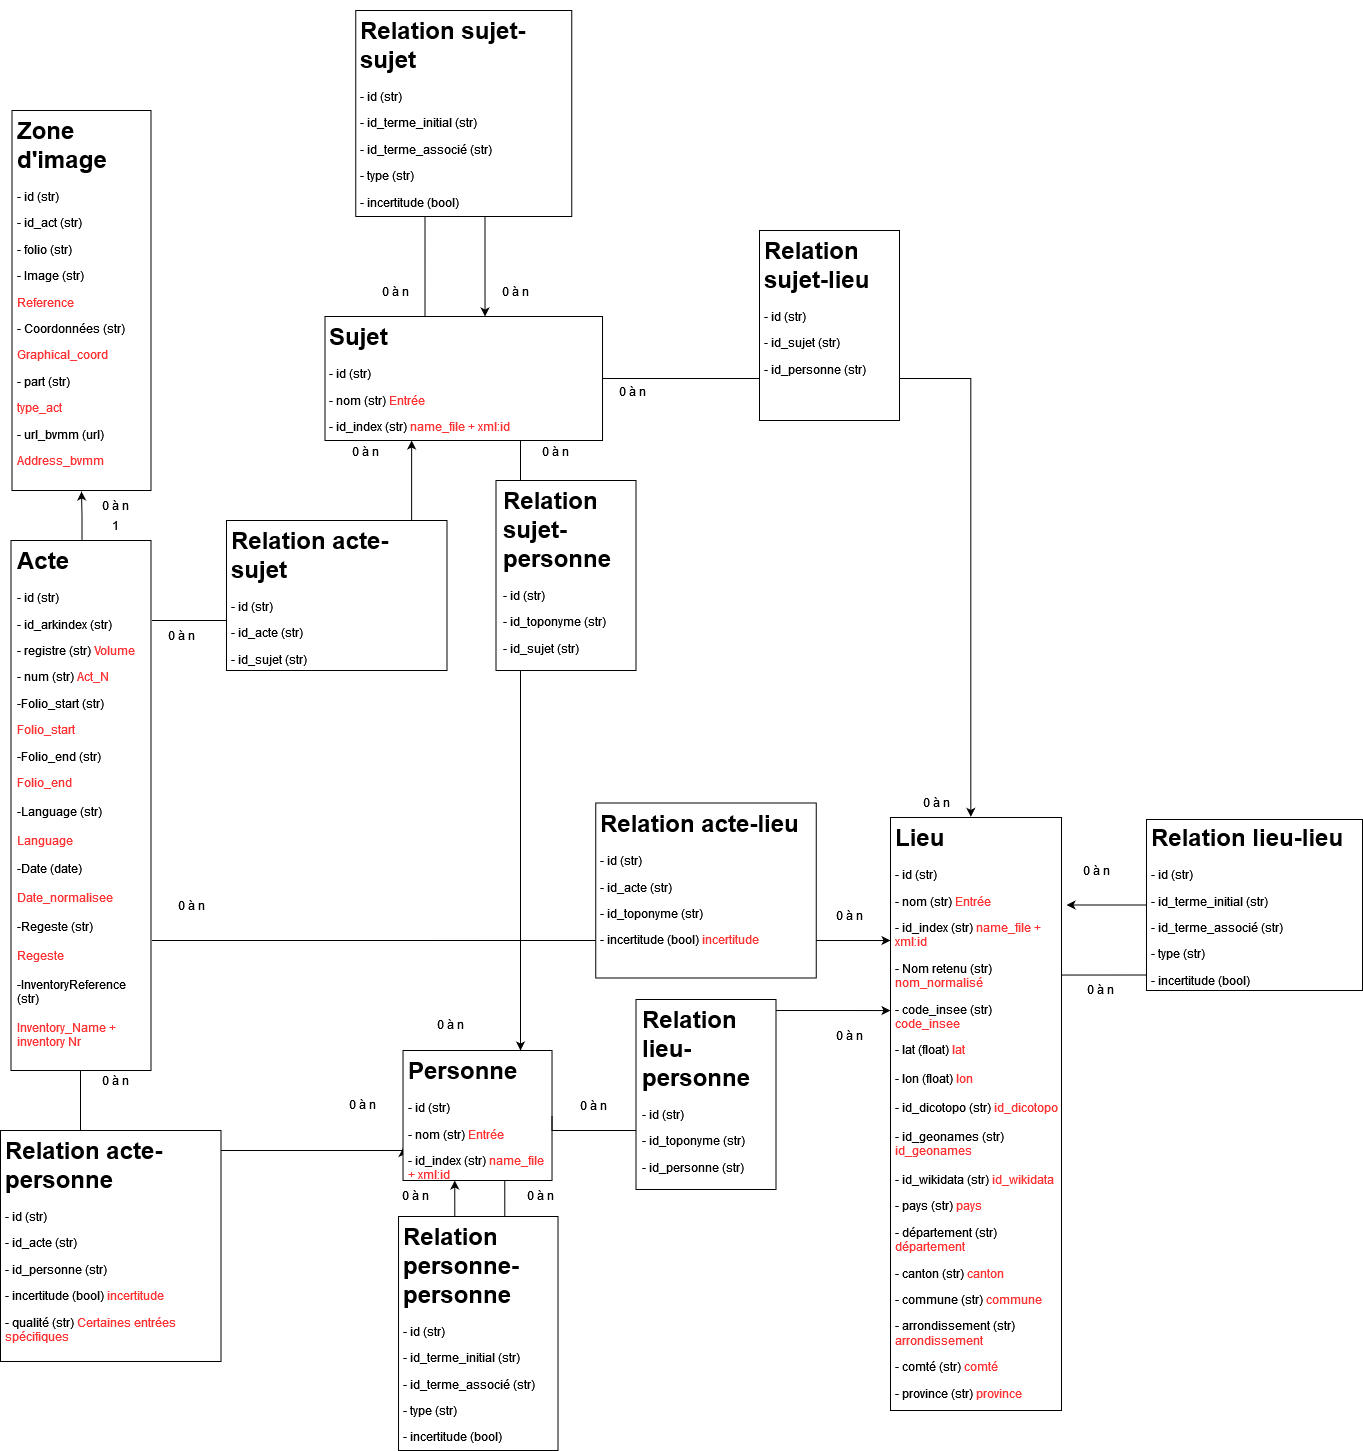
\includegraphics[width=\textwidth]{Images/modele_bd.png}
		\caption{Modèle de la base de données relationnelle permettant de décrire les registres du Trésor des chartes avec les zones d'images, les actes et les entités contenus dans les actes.}
		\label{Modele_bd}
	\end{figure}
	
	\subsection{L'import des données}
	
	Nous avons donc créé une base de données au sein de la plateforme Heurist\footnote{\url{https://heuristnetwork.org/}.} permettant la gestion de données issues de corpus en sciences humaine, leur diffusion et leur enrichissement collaboratif. La plateforme dispose d'un certain nombre de modèles de données déjà intégrés et personnalisables en fonction des besoins (Nous avons ici utilisé les entités \og Person\fg{} et \og Place\fg{}) et propose également d'en créer de nouveaux (Nous avons créé les entités \og Subject\fg{}, \og Act\fg{} et \og Image zone\fg{}). Elle propose aussi un modèle de relation N-N à partir de l'entité \og Record relationship\fg{}. Ces relations peuvent être qualifiées à l'aide d'un \og Relationship type\fg{} personnalisable et peuvent disposer d'attributs descriptifs.
	
	La préparation des données pour l'import a été réalisée en plusieurs étapes à l'aide d'un script python\footnote{\url{https://github.com/virgile-reignier/Memoire-TNAH-2022-Reignier/blob/main/Scripts/Index/upload_heurist.py}.}. La première étape consiste à créer à partir du fichier Excel les tables Person, Place et Subject et les importer dans Heurist. Il est alors possible de les exporter avec leurs identifiants local H-ID nécessaires à la construction des tables de relations. Elles sont au nombre de 6 : Person-Person, Person-Subject, Person-Place, Place-Subject, Place-Place, Subject-Subject. L'étape suivante consiste à utiliser le fichier JSON pour créer la table Act et l'importer dans Heurist. Les enregistrements de cette table sont ensuite exportés avec ses H-ID nécessaires pour construire la table Image zone et les tables de relation Act-Person, Act-Subject et Act-Place.
	
	\section{Le cas particulier des noms de lieu}
	
	\subsection{Segmentation des différentes parties de l'entrée}
	
	Importées au sein de la table Place de la base de données, les entrées toponymiques de l'index ont la particularité d'être composées de plusieurs éléments permettant de les localiser :
	
	 \begin{quotation}
	 	Lincques [Pas-de-Calais, con Guînes, cne Licques]
	 \end{quotation}
	
	
	\noindent La segmentation de ces éléments permet dans un premier temps de les intégrer parmi les attributs de la table. Il devient alors possible de filtrer les recherches en fonction de ces attributs. Cette segmentation est également un travail nécessaire pour aligner ces entités avec d'autres référentiels afin de les enrichir de coordonnées\footnote{Nous décrirons ce travail plus précisément au chapitre 7.}.
	
	Cette étape a été réalisée à partir du fichier CSV contenant les entrées d'index. Nous avons rédigé un script python afin de sélectionner automatiquement les entrées toponymiques et constituer un autre fichier au même format pour les traiter à part\footnote{\url{https://github.com/virgile-reignier/Memoire-TNAH-2022-Reignier/blob/main/Scripts/Index/toponymes.py}.}. Ce script permet ensuite de segmenter automatiquement les éléments qui composent l'entrée. La première étape de ce travail a été de former un élément \og entrée\fg{} permettant de simplifier son contenu et de faciliter l'alignement avec les autres référentiels. Cette forme simplifiée a été constituée par l'élimination des éléments de l'entrée situés entre crochets, puis par l'élimination des éléments restants placés après une virgule. Par exemple l'entrée :
	
	\begin{quotation}
		Sainte-Menehould, Sancta Manalhidis [Marne]
	\end{quotation}

	\noindent a pour forme simplifiée \og Sainte-Menehould\fg{}. Nous avons également créé un élément \og nom\_normalise\fg{} afin de proposer une forme du nom potentiellement plus facile à retrouver. Nous avons par exemple réinséré les particules devant le nom : L'entrée \og Sauvement (Le)\fg{} est ainsi transformée en \og Le Sauvement\fg{}. Nous avons également traité les noms composés dont certains morceaux peuvent parfois être glissés au sein des crochets. Ils sont alors repérable par la présence d'un \og - \fg{} : 
	
	\begin{quotation}
		Vailly [-sur-Aisne, Aisne, ar. Soissons]
	\end{quotation}
	
	\noindent nous avons dans ce cas reconstitué le nom complet : \og Vailly-sur-Aisne\fg{}. Il existe cependant ici une irrégularité dans la construction de ces noms composés : certains maintiennent l'espace présent habituellement avant le crochet ouvrant (comme l'exemple ci-dessus). D'autres sont au contraire construits au plus proche du nom composé et ne disposent pas de cet espace :
	
	\begin{quotation}
		Bar[-le-Duc, Meuse] , châtelain
	\end{quotation}
	
	La deuxième étape consiste ensuite à catégoriser automatiquement les différents éléments qui sont situés entre crochets. Ceux-ci peuvent être segmentés à partir des virgules qui sont utilisées comme séparateurs. Différents scénarios peuvent alors exister, mais le cas le plus courant est celui de \og Liucques\fg{} présenté plus haut. Le département est alors repéré par sa présence au sein d'une liste pré-établie, le canton par la chaîne de caractère \og con\fg{} et la commune par la chaîne \og cne\fg{}. Le résultat forme la table suivante :
	
	\begin{center}
		\begin{tabular}{|p{3cm}|p{3cm}|p{3cm}|p{3cm}|}
			\hline
			nom\_normalise & département & canton & commune \\ \hline
			Lincques & Pas-de-Calais & Guînes & Licques \\ \hline
		\end{tabular}
	\end{center}
	
	Le repérage des départements s'est ici confronté à deux difficultés. Tout d'abord un certain nombre d'entre eux sont mentionnés sous une forme abrégée comme \og Tarn-et-G.\fg{} ou \og Seine-Mme\fg{}. Nous les avons donc développées au fur et à mesure de la découverte de ces formes abrégées. Une autre difficulté repose sur les quelques évolutions administratives qui ont lieu depuis la parution de l'index. Ainsi le département \og Côtes-du-Nord\fg{} a par exemple changé de nom pour devenir \og Côtes-d'Armor\fg{}. Nous avons donc opéré la transformation automatiquement. Une situation plus complexe est celle de la réorganisation en 1968 des départements de la \og Seine\fg{} et \og Seine-et-Oise\fg{} pour former les 7 départements qui composent, avec la ville de Paris, l'actuelle région Île-de-France. Faute de pouvoir attribuer automatiquement un de ces nouveaux départements, nous avons conservé les anciens au sein du référentiel.
	
	Certaines entrées disposent également d'une indication à propos de l'arrondissement (marquée par \og ar.\fg{}). Cette indication, celle du canton et celle de la commune peuvent parfois être factorisées lorsque la ville concernée est la même :
	
	\begin{quotation}
		Osmeaux [Eure-et-Loir, ar. et con Dreux, cne Cherisy]
	\end{quotation}
	
	 Les entrées peuvent aussi disposer d'une forme actuelle du toponyme, elle est alors marquée à l'aide de l'indication \og auj.\fg{} :
	
	\begin{quotation}
		Genlis [auj. Viliequier-Aumont, Aisne, con Chauny] , monastère
		de Sainte-Élisabeth
	\end{quotation}

	\noindent Ou simplement par un nom différent de celui de l'entrée comme premier élément entre crochets :
	
	\begin{quotation}
		Agarne (L') [Notre-Dame-de-l'Agarne, Gard, con et cne Marguerittes]
	\end{quotation}
	
	\noindent Ces éléments ont la particularité de reprendre parfois certains mots de l'entrée, ils peuvent donc prendre une forme factorisée ou abrégée :
	
	\begin{quotation}
		Labastide-de-Montfort [auj. L.-de-Lévis, Tarn, con Gaillac]
	\end{quotation}
	
	\noindent Nous avons donc développés ces formes à la main (ici \og Labastide-de-Lévis\fg{}) pour disposer de la donnée entière. Lorsqu'elle est présente, cette forme actuelle a été utilisée comme valeur de l'attribut \og nom\_normalise\fg{}. Si la commune n'est pas précisée, nous avons aussi fait le choix d'entrer d'office la valeur de cet attribut dans l'attribut \og Commune\fg{}.
	
	Nous avons également dû prendre en compte un nombre conséquent de toponymes étrangers. Pour cette raison, nous avons ajouté un élément \og Country\fg{} dont la valeur est systématiquement \og France\fg{} sauf indication contraire. Nous avons créé un référentiel de pays, puis avons opéré une conversion au moment de l'import dans Heurist pour que le nom corresponde aux entités prédéfinies dans la plateforme. Certaines localités sont situées dans des pays qui ont cessé d'exister depuis (par exemple la Yougoslavie), mais leur nombre était assez faible pour que nous puissions chercher leur situation actuelle manuellement. Ces toponymes étrangers sont parfois agrémentés d'une précision sur la province où ils se situent (marquée par \og prov.\fg{}) ou sur le comté (marqué \og co.\fg{}) s'il s'agit d'un lieu en Grande-Bretagne\footnote{Ces toponymes étant au nombre de 12, leur existence nous avait échappé au moment de la rédaction de notre script. La segmentation de cet élément a donc été réalisée manuellement a posteriori.}.
	
	Un dernier problème se pose à partir des toponymes qui ne sont pas situés en un seul lieu. C'est le cas par exemple de certaines localités à cheval sur deux communes ou englobant deux communes, comme par exemple :
	
	\begin{quotation}
		Abbans [-Dessus et -Dessous, Doubs, con Boussières]
	\end{quotation}
	
	\noindent Nous avons dans ce cas conservé les deux entités dans la colonne correspondante (ici \og Abban-Dessus\fg{} et \og Abban-Dessous\fg{} sont des communes). Dans un second cas, la localité dispose d'indications permettant à l'index de la situer relativement :
	
	\begin{quotation}
		Le Maréchal (ferme qui fut à Richard) [près de Rouen]
	\end{quotation}
	
	\noindent Ces indications ne sont cependant pas suffisantes pour que l'on puisse retrouver précisément le lieu où aligner ces données avec d'autres référentiels. Pour cette raison, nous avons conservé les attributs \og Note\fg{} et \og Short summary\fg{} décrits précédemment afin de conserver l'ensemble des indications portées par l'index. Dans un dernier cas, le toponyme n'a pas pu être identifié avec certitude et plusieurs propositions sont formulées :
	
	\begin{quotation}
		Angles [Angle, Charente-Maritime, con Aulnay, cne Blanzay-sur-Boutonne, ou Anglas, Charente-Maritime, con Aulnay, cne Nuaillé-sur-Boutonne]
	\end{quotation}
	
	\noindent Dans ce cas, nous avons dédoublé l'entrée pour disposer des informations de localisation sur chacune des propositions et réaliser l'alignement.
	
	\subsection{Modéliser les lieux non-identifiés}
	
	Cette dernière situation a largement participé au questionnement que nous avons évoqué plus haut sur la modélisation d'une table pour les entrées d'index qui servirait d'interface entre les entités et les actes. Les propositions de localisation sont en effet des éléments qui ne sont pas superposables aux toponymes qui constituent l'entrée d'index, pourtant elles ne sont formulées que pour accompagner cette entrée toponymique. Nous avions imaginé un moment créer une table pour les lieux et une pour les localisations, mais il a finalement été convenu que chacune de ces propositions devienne une entité à part entière et distincte de celle formée à partir de l'entrée. Ces entités ont la particularité de ne pas être directement une entrée d'index et de n'être liées à aucun acte, elles sont simplement liées à leur entité de référence via une relation Lieu-Lieu. Contrairement aux cas de coordonnées multiples générées par l'alignement avec les référentiels externes, les propositions multiples de localisation présentes dans l'index sont encore à importer dans la base de données. Pour être complet dans la numérisation des indications de l'index, il faudrait également prendre en compte les marques d'incertitude dans les entrées d'index (généralement un \og ?\fg{}, nous les avons marqués dans le fichier CSV par une colonne \og incertitude\fg{}) et les reporter comme attribut de la relation entre l'entité correspondante de la base de données et l'acte auquel l'entrée d'index renvoi.
	
	\section*{Conclusion}
	
	Par ce chapitre, nous avons abordé le processus de transformation du fichier TEI contenant les entrées d'index en une base de données relationnelle. Nous avons pour cela décrit dans un premier temps les étapes de préparation de ce travail par la transformation préalable du fichier TEI en un fichier au format CSV puis Excel et par la description des attributs des tables. Nous avons ensuite décrit la mise en place du modèle relationnel à travers la modélisation de la table et le travail d'import. Pour finir, nous avons exposé le cas spécifique des entrées toponymiques au travers des problèmes de segmentation et de modélisation des lieux non-identifiés.
	
	La création de cette base de données relationnelle constitue donc une forme d'aboutissement de notre travail de stage puisqu'elle prend en compte tous les éléments que nous avons décrit auparavant. Nous verrons cependant aux chapitres suivants comment ce travail a pu être enrichi par l'ajout de lien avec les autres données du projet et avec des ontologies web. Avec cette base de données, nous disposons donc d'un référentiel complet mis en ligne sur la plateforme Heurist et librement utilisable pour la suite de ce travail. Le choix de la plateforme permet également de favoriser la publication de ce travail, mais aussi son accroissement futur par l'ajout de nouvelles entrées au sein du référentiel.
	
	\chapter*{Conclusion partielle}
	
	Après une première partie consacrée au contexte de travail dans lequel nous avons réalisé notre stage, cette seconde partie nous a permis d'exposer toutes les étapes de la construction du référentiel d'entités nommées destiné à produire les données d'entraînement pour l'apprentissage du liage d'entités. Notre développement a commencé par un premier chapitre consacré au travail de compréhension des \textit{legacy data} constituées par l'index et aux difficultés liées à leur traitement numérique. Ensuite, nous avons dédié un second chapitre aux différentes relations qui caractérisent les entrées d'index et à leur prise en compte dans la construction du référentiel. Nous avons enfin terminé cet exposé par une troisième partie portant sur la modélisation et la concrétisation du référentiel sous la forme d'une base de données relationnelle. Nous disposons donc aujourd'hui d'un ensemble d'entités prêtes à être utilisées pour le liage avec les entités nommées présentes dans les registres concernés.
	
	Ce long travail nous a permis de voir que la réutilisation de \textit{legacy data} dans un cadre numérique est associée à certain nombre de problématiques qui freinent largement ce processus. Chaque étape doit en effet prendre en compte un grand nombre d'exceptions, qu'elles viennent de l'ouvrage en lui-même ou d'erreurs réalisées au cours de la chaîne de traitement. Ces problématiques sont à l'origine d'une réduction conséquente de l'ambition du stage. Nous avions en effet envisagé dans un premier temps poursuivre ce travail de transformation des index avec ceux des inventaires des registres JJ 65 à JJ 79B puis avec ceux des inventaires géographiques. Au vu du temps consacré à la transformation du premier ouvrage, il a été décidé de se concentrer sur celui-ci pour aller le plus loin possible et fournir une base de travail aux prochains travaux sur ce corpus.
	
	\parttext{Si la constitution d'un référentiel à partir d'entrées d'index constitue l'objectif premier du stage, ce travail n'est pas suffisant pour fournir un outil pertinent afin d'étudier le contenu du Trésor des chartes. Les données constituées, pour être utiles, doivent en effet pouvoir rejoindre et compléter les différentes ontologies web déjà disponibles. Nous consacrerons donc cette troisième et dernière partie à la création de liens à partir du référentiel et à ses utilisations. L'objectif étant de l'insérer dans les connaissances générales disponibles sur les documents historiques. Pour cela, nous décrirons dans un premier chapitre le processus d'enrichissement du référentiel par son alignement avec des ontologies web. Puis nous dédierons un second chapitre à la mise à disposition du référentiel et aux liens réalisés avec les autres données du corpus. Enfin, nous consacrerons un troisième chapitre aux différents essais réalisés pour la mise en œuvre du liage d'entités.}
	
	\part{Alignement, diffusion et utilisation du référentiel}
	
	\chapter{Enrichir les données à l’aide d’un référentiel externe}
	
	Nous disposons à l'heure actuelle d'une table au format CSV contenant les toponymes identifiés dans les registres JJ 37 à JJ 50 du Trésor des chartes. Nous avons pour cela utilisé l'index de l'inventaire analytique de ces registres. De plus, nous avons segmenté les différents éléments présents dans ces entrées toponymiques de l'index et en avons notamment extrait les circonscriptions administratives qu'elles contiennent. Il manque cependant un élément pour localiser précisément ces entités : des coordonnées. Celles-ci ne sont en effet pas présentes dans l'index, nous devons donc aller les chercher dans un référentiel externe pour permettre l'enrichissement des toponymes contenus dans notre base de données.
	
	Ce chapitre sera donc consacré au travail d'alignement entre les données de l'index et plusieurs référentiels en ligne pour permettre la sélection de coordonnées et enrichir ces données. Pour cela, nous présenterons dans un premier temps les interfaces que nous avons utilisées. Puis nous exposerons le processus de construction des requêtes utilisé pour obtenir les coordonnées. Enfin, nous décrirons différents cas spécifiques qui se sont présentés à nous au cours de ce travail.
	
	\section{Présentation des référentiels utilisés}
	
	\subsection{GeoNames}
	
	Parmi les référentiels géographiques mobilisables pour enrichir des toponymes de coordonnées, GeoNames (\url{https://www.geonames.org/}) dispose de plusieurs qualités essentielles pour notre travail : les données sont libres de droit, elles couvrent le monde entier et chaque entité dispose d'un identifiant unique permettant de le retrouver en cas de besoin. Outre l'interface web permettant de naviguer parmi les localités, le site dispose également d'une API pour faciliter la récupération automatique d'information\footnote{\url{https://www.geonames.org/export/web-services.html}.}. Cette API est un service client qui nécessite de s'inscrire sur le site pour disposer d'un compte utilisateur. Ce compte permet ensuite d'adresser des requêtes qui retournent la donnée correspondante sous format XML (\textit{cf}. figure \ref{API_geonames}). Quelques limites sont à prendre en considération pour les comptes gratuits : la taille des réponses est limitée à 500 lignes et le nombre de requêtes à 1 000 par heure et 20 000 par jour. Les besoins de notre travail permettent de s'accommoder assez facilement de ces contraintes, notamment par l'ajout d'un minuteur lorsque le retour d'une requête indique que la limite est dépassée. La fonction python \og time.sleep\fg{} permet de mettre l'exécution du programme en pause le temps nécessaire.
	
	
	\begin{figure}
		\centering
		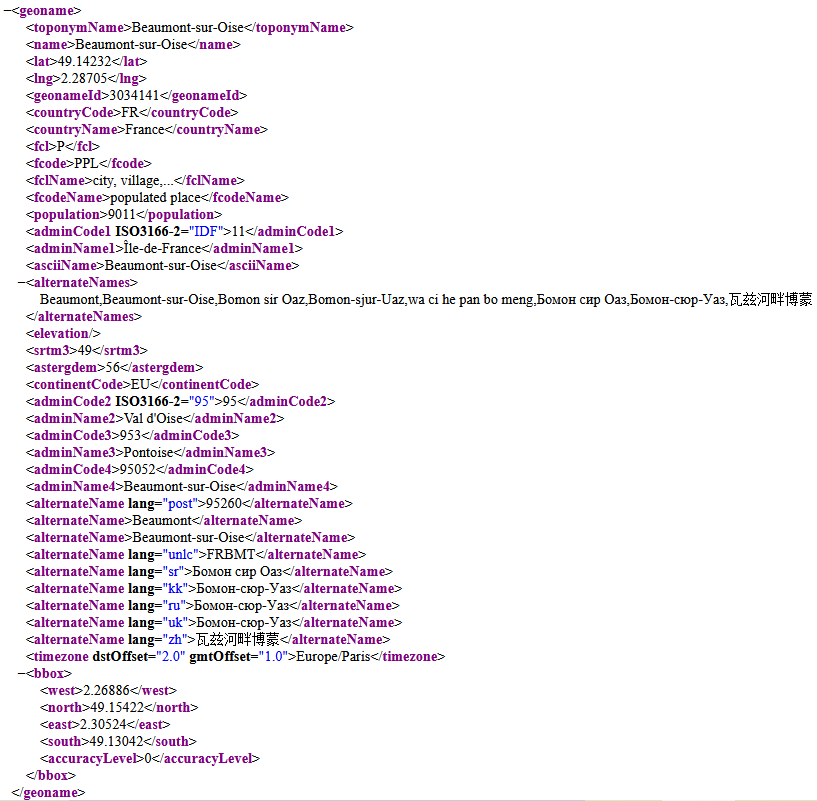
\includegraphics[width=\textwidth]{Images/Result_geonames.png}
		\caption{Exemple de retour de l'API GeoNames.}
		\label{API_geonames}
	\end{figure}
	
	
	GeoNames est donc l'outil le plus complet pour travailler sur des localités françaises et étrangères. Les subdivisions administratives et leurs codes sont respectivement encodés dans des balises <adminName[N]> et <adminCode[N]> où [N] est le rang de la subdivision. Cette méthode permet de disposer d'un encodage unique pour toutes les localités et facilité la navigation d'un pays à un autre. Néanmoins, ces balises ne sont pas accompagnées d'un attribut permettant de savoir à quelle entité administrative correspond chaque donnée (département, région, conté, province, ...), ce qui limite la précision des recherches pour certains pays.
	
	\subsection{DicoTopo}
	
	Le \textit{Dictionnaire topographique de la France} est un projet mené depuis 1859 par le CTHS. Son objectif est de collecter l'ensemble des noms de lieu français dans leur graphie ancienne et moderne. Publié sous la forme d'un volume par département, ce travail encore inachevé a permis de rendre disponible un ensemble conséquent de données sur les localités situées dans 35 départements français. Depuis 2010, le CTHS a entrepris de rendre disponible ces données sous format numérique à l'aide d'une application dédiée (\url{https://dicotopo.cths.fr/}). Elle fournit donc à ce jour l'outil disponible le plus précis pour chercher des localités à l'échelle infra-communale et des formes anciennes de toponyme. L'application DicoTopo dispose elle aussi d'une API librement utilisable à l'aide de requêtes qui retournent un résultat au format JSON (\textit{cf}. figure \ref{API_dicotopo}).
	
	\begin{figure}
		\centering
		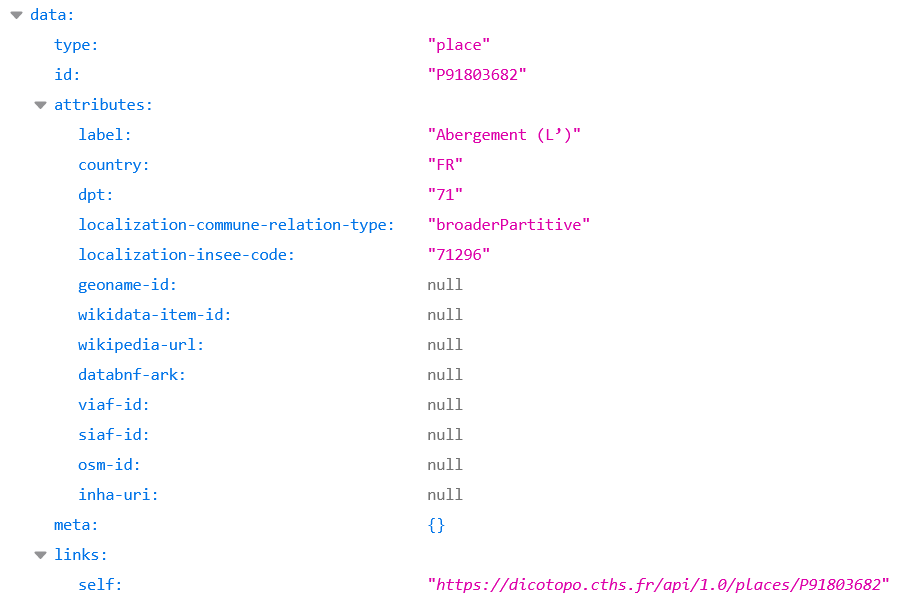
\includegraphics[width=\textwidth]{Images/Result_dicotopo.png}
		\caption{Exemple de retour de l'API DicoTopo.}
		\label{API_dicotopo}
	\end{figure}
	
	Contrairement à GeoNames, l'API de DicoTopo ne dispose d'aucune limite dans son utilisation\footnote{\url{https://dicotopo.cths.fr/documentation}.}. De plus, la présence de localités infra-communales et de formes anciennes rendent cet outil plus adapté que GeoNames pour retrouver les lieux mentionnés dans le Trésor des chartes. La principale limite de l'application réside donc dans le caractère inachevé du travail de collecte. Pour cette raison, nous avons fait le choix d'utiliser en priorité DicoTopo pour les lieux situés dans les départements couverts par l'application et d'utiliser GeoNames pour ceux situés hors de France ou dans les départements non-couverts.
	
	\section{Construction de la requête}
	
	\subsection{Choisir le nom à chercher}
	
	La recherche des toponymes a donc été réalisée à l'aide d'un algorithme python permettant d'écrire les requêtes en fonction des situations\footnote{\url{https://github.com/virgile-reignier/Memoire-TNAH-2022-Reignier/blob/main/Scripts/Index/geonames.py}. Lire aussi \cite{reignier_lindex_2022}.}. Une étape centrale consiste à vérifier si le toponyme est situé dans un département couvert par DicoTopo car elle détermine la suite de la procédure. Le cas échéant, la requête est construite à partir de l'url \og https://dicotopo.cths.fr/api/1.0/search?query=label: \fg{} suivie du nom du lieu recherché. La réponse comprend toutes les entités du référentiel contenant ce nom. Des filtres sont donc opérés pour trier ces entités en fonction du département ou de la commune s'ils sont indiqués par l'index. Si aucune commune n'est indiquée, toutes les entités portant ce nom dans le département sont conservées comme des localisation potentielles. Par la suite, toutes les entités retenues sont transformées sous la forme d'un élément liste contenant leurs codes insee, leurs coordonnées et leurs identifiants dans DicoTopo.
	
	Si le toponyme n'est pas situé dans un département couvert par DicoTopo, la recherche est effectuée sur l'API GeoNames. La requête est construite différemment : au lieu de filtrer les entités contenues dans la réponse en fonction du département ou de la commune, nous avons mis en place les filtres dès la requête afin de prendre en compte les limites posées par l'interface. La requête est construite sous la forme : \og http://api.geonames.org/ search?style=FULL\&name=[NAME]\&username=[USERNAME]\fg{} où [NAME] correspond au nom du toponyme et [USERNAME] à l'identifiant du compte utilisateur. Les arguments supplémentaires sont ensuite \og country=[COUNTRY]\fg{} où [COUNTRY] correspond au pays et \og adminCode2=[NUM]\fg{}. Dans le contexte d'un toponyme français, [NUM] correspond au numéro du département. Des filtres sont néanmoins opérés pour vérifier que le nom correspond bien à celui recherché ou au moins à un élément du nom\footnote{Il arrive parfois que des parties du nom de la commune soient modifiées au cours du temps. Par exemple la ville de Mantes-la-Jolie actuellement dans les Yvelines s'appelait simplement Mantes au moment de la parution de l'index.} (la comparaison est également étendue au contenu des balises <alternateName>) et pour ne garder qu'une seule entité par commune. Comme avec DicoTopo, les entités retenues sont ensuite transformées sous la forme d'un élément liste contenant leurs codes insee, leurs coordonnées et leurs identifiants GeoNames. Pour les localités dont le département renseigné correspond à \og Seine\fg{} ou \og Seine-et-Oise\fg{}, la recherche doit être adaptée au contexte actuel. Les communes des deux anciens départements ayant été réparties entre les 6 nouveaux (Yvelines, Val-d'Oise, Essonne, Hauts-de-Seine, Seine-Saint-Denis, Val-de-Marne)\footnote{A l'exception de la commune de Paris qui forme une collectivité autonome.}, les requêtes doivent être démultipliées pour chercher le toponyme dans chacun des départements correspondants.
	
	Il faut également prendre en compte des ambiguïtés parfois présentes entre l'entrée de l'index, la forme actualisée du nom et la commune. Malgré les catégorisations que nous avons présentées au chapitre 6, il est parfois délicat de différencier automatiquement des formulations similaires :
	
	\begin{quotation}
		Mauves-sur-Huine [Orne, con Mortagne]
	\end{quotation}

	\begin{quotation}
		Mauvers [Tarn-et-Garonne, con Verdun, cne Aucamville]
	\end{quotation}

	\begin{quotation}
		Mazis-Bocquet (Les) [Les Mazis, Seine-Maritime, con Neufchâtel, cne Saint-Saire]
	\end{quotation}

	\begin{quotation}
		Molerie [Molières, Tarn-et-Garonne, ar. Montauban] , homines et universitas
	\end{quotation}
	
	
	\noindent Dans le premier cas, Mauves-sur-Huine correspond à une commune dans l'Orne. Dans le second cas, Mauvers est une localité située dans la commune d'Aucamville dans le Tarn-et-Garonne. Dans le troisième cas, Les Mazis Bocquet est une forme ancienne de la localité Les Mazis située dans la commune de Saint-Serre en Seine-Maritime. Dans le troisième cas, Molerie est une forme ancienne de la commune de Molières dans le Tarn-et-Garonne. On peut donc voir que la place du mot comme entrée index ou comme premier élément entre crochet ne suffit pas à définir sa sémantique. Il faut donc réaliser plusieurs tests successifs pour s'assurer que la recherche sur les API trouve la bonne localité ou aligner le toponyme avec la commune dans laquelle il est situé en cas d'absence dans le référentiel.
	
	Pour cela, nous avons établi une recherche préliminaire basée sur la commune lorsqu'elle est renseignée afin de disposer de ses coordonnées. Cette recherche est effectuée sur l'API GeoNames car celle-ci dispose d'un argument de recherche dédié aux entités disposant d'un code postal : \og postalCodeSearch? \fg{}. La recherche s'effectue ensuite de la même manière que celle décrite précédemment, à ceci près que la réponse ne contient pas l'identifiant GeoNames de l'entité. Il faut donc construire une nouvelle requête à partir du résultat de la dernière sur le modèle \og http://api.geonames.org/search?style=FULL \&q=[POSTALCODE]\&name=[NAME]\&username=[USERNAME]\fg{} pour obtenir toutes les indications voulues sur la commune. Ici, l'utilisation de [POSTALCODE] permet de s'assurer que la commune contenue dans le retour est bien la même que celle trouvée avec la requête précédente. Si jamais la commune n'est pas trouvée dans GeoNames et qu'elle se situe dans un département couvert par DicoTopo, alors une tentative est également effectuée via son API.
	
	Cette étape permet ainsi de prendre en compte les différents éléments contenus dans les entrées. La recherche par toponyme est ainsi réalisée uniquement s'il est différent du nom de la commune. Si jamais la réponse ne contient pas de résultat satisfaisant, une nouvelle recherche est effectuée à partir de l'élément \og nom\_normalise \fg{}. Si aucune des deux ne permettent d'obtenir un résultat, alors les éléments extraits de la recherche par commune sont conservés pour enrichir le toponyme.
	
	\subsection{Récupération des coordonnées}
	
	Le résultat de ce processus est ensuite enregistré dans un fichier CSV qui reprend les éléments contenus dans le fichier formé à partir de la segmentation des entrées toponymiques (\textit{cf}. Chapitre 6) accompagné de colonnes supplémentaires pour y insérer le code insee, la latitude, la longitude et l'identifiant de l'entité dans le référentiel utilisé. De plus, le résultat des requêtes a été complété par une série de messages d'erreur permettant de suivre certains résultats associés aux différentes étapes du processus. Ces indications nous ont permis d'améliorer la rédaction de notre algorithme par le suivi de certaines variables et de leur adéquation avec les données sources.
	
	Dans la plupart des cas, le résultat de ce processus permet d'associer chaque entrée d'index à une série complète de données supplémentaires. Mais quelques cas spécifiques peuvent se présenter : les localités étrangères ne disposent pas de code insee et quelques entités renseignées par DicoTopo ne disposent pas de coordonnées. Il arrive également que certaines localités ne disposent pas de coordonnées propres et s'étendent sur plusieurs communes :
	
	\begin{quotation}
		Canteloup (fief de) [Calvados, ar. et con Lisieux, cnes Marolles et Fumichon]
	\end{quotation}

	Dans ce cas, les coordonnées associées au toponyme sont celles des deux communes Marolles et Fumichon. Cette situation est ici à distinguer des situations d'incertitude : dans ce dernier cas la multiplication des coordonnées correspond à la présence d'hypothèses différentes pour situer le lieu. Au contraire, la présence de coordonnées multiples signifie ici que l'entité s'étend sur la surface de plusieurs entités dans le référentiel utilisé. Nous avons donc ajouté une colonne \og étendue\fg{} afin de pouvoir opérer cette distinction. Au moment de l'import des données dans Heurist, les coordonnées retenues des toponymes correspondant à cette situation sont calculées à partir de la moyenne des valeurs présentes dans les colonnes \og latitude\fg{} et \og longitude\fg{}. Dans le cas où ce sont des communes, tous les codes insee sont importés dans Heurist.
	
	Comme exposé au chapitre 5, les sous-entrées dépendant d'entrées toponymiques n'ont pas pu être différenciées les unes des autres et ont toutes été catégorisées comme relevant du type \og lieu \fg{}. En suivant cette logique, nous avons systématiquement enrichi chacune de ces sous-entrées avec les coordonnées de l'entité donc elles dépendent. Il arrive cependant que quelques unes de ces sous-entrées correspondent à des entités qui disposent de coordonnées propres :
	
	\begin{quotation}
		Bacqueville [Eure, con Fieury-sur-Andelle] , — forêt [Eure, con
		Fleury-sur-Andelle, cnes Bacqueville et Radepont]
	\end{quotation}
	
	Comme nous ne les avions pas identifiés au moment de la création du fichier CSV préliminaire au travail d'alignement, nous les avons repérés \textit{a posteriori} par la présence de crochets après le séparateur \og , — \fg{} et avons procédé manuellement à leur alignement avec les référentiels GeoNames et DicoTopo. Dans cette situation, ces coordonnées ont été préférées à celles de l'entrée générale au moment de l'import dans Heurist.
	
	\section{Gestion des cas spécifiques}
	
	\subsection{Résoudre les ambiguïtés}
	
	Comme nous l'avons vu, la prise en compte des différentes possibilités de composition des entrées nous a poussés à tester plusieurs scénarios au moment de la construction des requêtes. Nous avons ainsi dû arbitrer entre une récupération large de résultats pour s'assurer de trouver la bonne entité et des filtres efficaces afin de limiter la présence d'entités superflues. Malgré nos efforts, un certain nombre de reprises ont été effectuées. C'est le cas notamment des requêtes opérées sur DicoTopo dont les retours contiennent régulièrement des doublons que nous avons dû éliminer. Quant à GeoNames, le retour des requêtes contient parfois plusieurs résultats pour une même entité. C'est le cas par exemple des communes françaises qui sont référencées à la fois comme des lieux d'habitation et comme des circonscriptions administratives (\textit{cf}. figure \ref{Double_retour_GeoNames}). Nous avons fait ici le choix d'éliminer systématiquement les circonscriptions administratives lorsqu'il existe une autre entité portant le même nom. Cette situation se retrouve également pour un certain nombre de grandes villes étrangères dont le nom est le même que celui de l'entité administrative qui la contient (par exemple la ville de Milan est le chef-lieu de la ville métropolitaine de Milan qui contient 134 communes).
	
	\begin{figure}
		\centering
		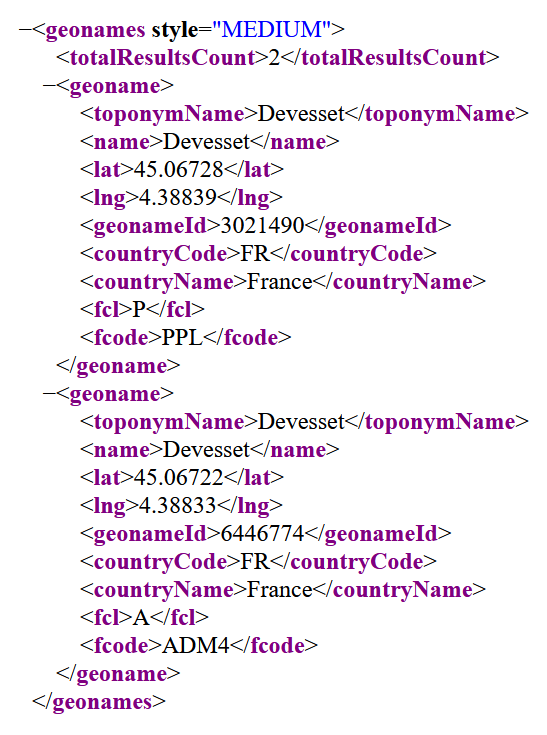
\includegraphics[width=8cm]{Images/town_on_geonames.png}
		\caption{La recherche pour la commune \og Devesset\fg{} dans GeoNames renvoie deux entités : une pour la ville et une pour la circonscription administrative}
		\label{Double_retour_GeoNames}
	\end{figure}
	
	 D'autres ambiguïtés sont présentes à partir de certaines rivières dont le nom est présent dans celui de plusieurs communes riveraines ou dans le nom d'un département (par exemple la rivière Allier donne son nom au département éponyme ainsi qu'à la commune Varennes-sur-Allier). De la même manière le nom de certaines régions historiques est encore porté dans celui de quelques communes (par exemple Laurac-en-Vivarais, située dans le Vivarais historique). Pour éviter les ambiguïtés, nous avons repris manuellement l'ensemble de ces entrées (repérées par la présence de mots-clefs comme \og pays\fg{}, \og rivière\fg{}, \og région\fg{}, ...) pour vérifier que les entités avec lesquelles elles ont été alignées correspondent bien à celles voulues. Une fois ce travail accompli, il reste encore quelques ambiguïtés issus du processus d'alignement qui n'ont pas pu être résolues de manière automatique ou semi-automatique\footnote{A ce propos, v. aussi \cite{reignier_lindex_2022}.}. Nous avons donc conservé chacune des entités issues du processus d'alignement et les avons considérés de la même manière que les propositions de localisation formulées par l'index au moment de l'import dans Heurist\footnote{\textit{Cf}. chapitre 6.}.
	
	\subsection{Les régions historiques}
	
	Parmi les cas particuliers présents dans notre corpus, les régions historiques sont particulièrement difficiles à aligner avec des coordonnées\footnote{A ce propos, v. aussi \cite{mcdonough_named_2019}.}. Si certaines d'entre elles sont présentes en tant que telles dans GeoNames ou DicoTopo (par exemple l'Armagnac, GeoNames ID 3036926), d'autres ont été alignées avec la commune qui constituait le chef-lieu :
	
	\begin{quotation}
		Termenès [pays de l'Aude dont Termes était le chef-lieu] ,
		juge
	\end{quotation}

	\noindent L'entité \og Termenès\fg{} a été dotée d'un attribut \og Name chosen\fg{} avec pour valeur \og Termes\fg{} et les coordonnées choisies pour l'entité  sont celles du chef-lieu. Nous avons également pu trouver quelques coordonnées supplémentaires dans Wikidata comme par exemple pour le Léon (Wikidata ID  Q12178). Un dernier cas spécifique est celui des régions historiques situées à cheval entre plusieurs pays actuels :
	
	\begin{quotation}
		Quatre-Métiers (les) [partie de la Flandre relevant de l'Empire
		et composée des paroisses d'Hulst (Pays-Bas, prov. Zélande), Axel (idem),
		Bouchaute (Belgique, prov. Flandre orientale) et Assenede (idem)]
	\end{quotation}

	\noindent Cette région est présente dans Wikidata (Q2789324), mais ne dispose pas de coordonnées. Nous avons donc aligné l'entité avec cet identifiant, ainsi qu'avec celui des communes d'Hulst, Axel, Bouchate et Assenede dans GeoNames et nous avons calculé des coordonnées à partir de la moyenne des coordonnées de ces communes.
	
	Nous avons également été confronté à quelques ambiguïtés dans les formulations proposées par l'index :
	
	\begin{quotation}
		Dunois (le) [région de Dun, Ariège, con Mirepoix] ,
		châtelain
	\end{quotation}

	\begin{quotation}
		Rabonitum [Ariège, région Pamiers]
	\end{quotation}

	\noindent Si la première entrée correspond sans conteste à une région dont le chef-lieu est Dun, la seconde correspond \textit{a priori} à une localité située près de Pamiers sans que la distinction entre les deux possibilités ne puisse être définie de manière certaine.
	
	\section*{Conclusion}
	
	Ce chapitre nous a permis d'aborder les différentes étapes du travail d'alignement entre les entités créées à partir de l'index et plusieurs référentiels en ligne disposant de coordonnées. Nous avons pour cela présenté les caractéristiques des deux principaux outils que nous avons utilisés, puis nous avons décrit le processus de construction de la requête à partir des différents noms à chercher et le choix des coordonnées récupérées, enfin nous avons exposé les différents cas spécifiques qui se sont présentés au cours de notre travail.
	
	Cette étape constitue donc la dernière de la mise en place du référentiel d'entités nommées destiné à nourrir l'entrainement d'un modèle de liage d'entités sur les actes du Trésor des chartes. Les données toponymiques ainsi enrichies ont pu compléter les éléments importés sur Heurist. Ces coordonnées permettent également d'envisager de dépasser le simple cadre du travail sur le liage d'entités. Les données ainsi localisées permettent en effet de dresser un certain nombre de visualisations cartographiques à partir des données du Trésor des chartes et utilisables à des fins multiples.
	
		
	\chapter{Mise à disposition d'un nouveau référentiel}
	
	Une fois constituée, la base de données Heurist contenant les entités décrites par l'index accompagnant l'inventaire analytique des registres JJ 37 à JJ 50 du Trésor des chartes peuvent être utilisées pour plusieurs usages. Si certains sont liés directement aux techniques de lecture automatique des textes, d'autres concernent plus directement le contenu des documents. Cet outil permet par exemple de faire des études croisées sur l'utilisation d'une notion ou de visualiser l'évolution du lien entre le pouvoir royal et une région au cours de la période. Il paraît donc nécessaire de rendre ces données disponibles aux usagers qui sont intéressés par le contenu de ces archives et qui souhaiteront les réutiliser dans leurs propres recherches.
	
	Ce chapitre sera donc consacré au travail de mise à disposition des données manipulées pendant le stage afin de faciliter leur usage pour la suite du projet et pour la communauté scientifique. Pour cela, nous détaillerons dans un premier temps les éléments mis en ligne pendant le stage et les liens visibles entre les différents fichiers. Puis nous présenterons les différentes visualisations cartographiques permises par la présence de coordonnées. Enfin, nous rendrons compte du travail préparatoire à la suite du projet par l'import des données sur Arkindex.
	
	\section{Mise en ligne des données collectées}
	
	\subsection{Des compléments au dépôt Github}
	
	Le travail réalisé au cours du stage à partir de l'index nous a permis d'enrichir les données déjà en ligne sur le dépôt Github du projet Himanis (\url{https://github.com/oriflamms/himanis}). Nous y avons notamment ajouté le fichier XML final contenant les entrées d'index\footnote{\url{https://github.com/oriflamms/himanis/blob/master/Inventories/Systematic/Paris_AN_JJ_inventaire_JJ37-50_index.xml}.}. Ce fichier permet notamment de montrer un état intermédiaire de la transformation de l'index car il est construit de manière linéaire et contient l'ensemble des éléments présents dans la publication papier. De plus, chaque entrée utilisée par la suite dispose d'un identifiant unique et de liens visibles avec les autres entrées avec laquelle elle est associée. Nous avons également ajouté dans le même dépôt le fichier Excel utilisé pour l'import des données dans Heurist\footnote{\url{https://github.com/oriflamms/himanis/blob/master/Inventories/Systematic/Paris_AN_JJ_inventaire_JJ37-50_index.xlsx}.}.
	
	Ce travail a également été l'occasion de mettre à jour le fichier XML contenant les entrées de l'inventaire\footnote{\url{https://github.com/oriflamms/himanis/blob/master/Inventories/Systematic/Paris_AN_JJ_inventaire_JJ37-50.xml}.}. Nous avons en effet décrit au chapitre 3 le travail de mise à plat des entrées d'index au sein de l'inventaire qui avait été réalisé dans les précédentes étapes du projet (\textit{cf}. figure \ref{index_in_inventaire}). Nous avons donc procédé à l'élimination systématique des entrées d'index ajoutées dans les entrées d'inventaire. Nous avons cependant conservé un certain nombre d'éléments de type \og subject \fg{} car ils ne sont pas directement issus de ce travail de mise à plat mais de l'exploitation d'un tableau produit par les Archives Nationales. Ces entrées ont été transformées de manière différentes et des comparaisons pourront être réalisées avec les éléments contenus dans la base de données. Le résultat prend la forme d'une balise <index> au contenu allégé comme présenté par la figure \ref{Subjects_in_inventory}.
	
	\begin{figure}
		\centering
		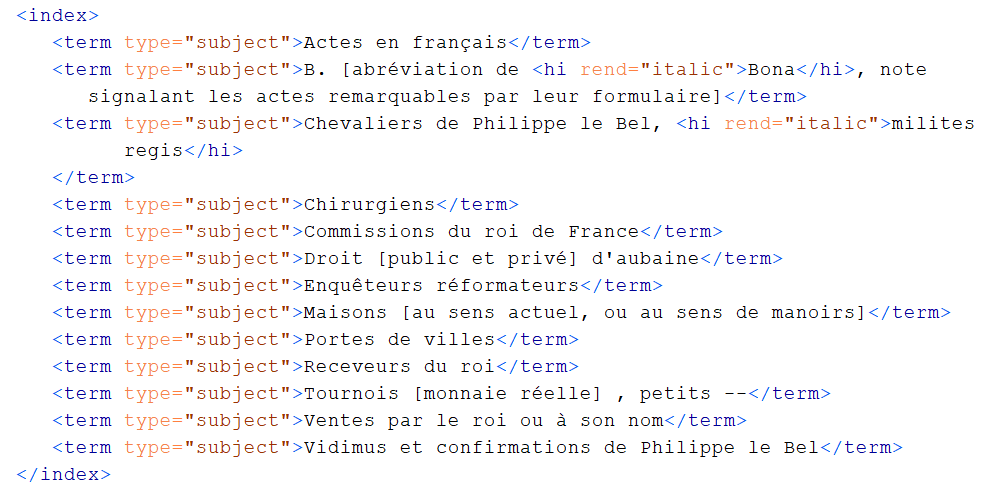
\includegraphics[width=\textwidth]{Images/Subects_in_inventaire.png}
		\caption{Exemple d'entrées d'index insérées dans une entrée d'inventaire après suppression des éléments issus du fichier XML pour ne laisser que ceux issus du tableau des Archives Nationales.}
		\label{Subjects_in_inventory}
	\end{figure}
	
	\subsection{Des liens visibles entre les données}
	
	La mise en ligne de la base de données sur la plateforme Heurist permet d'envisager la diffusion du référentiel à large échelle et la démultiplication de ses usages. Cependant, les données manipulées ne forment pas actuellement l'état final visé\footnote{Nous avons formulé quelques propositions d'amélioration au sein de l'annexe C.}. Leur publication est donc encore à l'état de projet. Nous avons toutefois pensé les données importés dans Heurist en fonction de cette mise à disposition future. Pour cette raison, un attribut \og Index reference\fg{} a été ajouté aux entités Place, Person et Subject pour les associer aux entrées d'index au sein des fichiers de travail. Cet attribut est construit à partir du nom du fichier contenant cette entrée d'index et de l'identifiant de l'entrée en question, sous la forme :
	
	
	\begin{quotation}
		Paris\_AN\_JJ\_inventaire\_JJ37-50\_index.xlsx\#d1e132079
	\end{quotation}
	
	De la même manière, les entrées de la table Act disposent d'un attribut \og Inventory Reference\fg{} qui contient le nom du fichier contenant cette entrée d'inventaire et le numéro de l'acte dans le même inventaire sous la forme :
	
	\begin{quotation}
		Paris\_AN\_JJ\_inventaire\_JJ37-50.xml\#433
	\end{quotation}
	
	\noindent Ces éléments permettent de faciliter le suivi des données depuis les documents sources vers la base de données afin de retracer les différentes étapes de sa transformation et de retrouver les incohérences qui pourraient s'y être glissées. Ce suivi paraît particulièrement pertinent en cas d'ouverture de la base de données au \textit{crowdsourcing} car il permettra à chacun de vérifier la cohérence des données avec les documents sources et de proposer les ajouts ou corrections qu'il jugera nécessaire.
	
	\section{Un résultat direct : visualiser les lieux mentionnés dans les registres JJ 37-60}
	
	\subsection{Visualisation des lieux décrits par l'index sous forme d'une carte de chaleur}
	
	L'alignement des entrées toponymiques avec des référentiels externes pour les enrichir de coordonnées permet d'apporter une dimension spatiale à l'index. Chacune de ces entités peut en effet être projetée sur une carte et offrir autant de visualisation du contenu des registres. Nous avons donc travaillé à la production d'une carte de chaleur permettant une visualisation complète des lieux mentionnés par l'index. Cette réalisation permet à la fois de montrer un état de notre travail en cours et de proposer une cartographie des lieux mentionnés dans les registres JJ 37 à 50 du Trésor des chartes et donc concernés d'une manière directe ou indirecte par l'action du roi entre 1303 et 1314. Cette carte a été réalisée à l'aide d'un script python\footnote{\url{https://github.com/virgile-reignier/Memoire-TNAH-2022-Reignier/blob/main/Scripts/Index/carte_toponymes.py}.} et est disponible à l'adresse suivante : \url{https://virgile-reignier.github.io/Carte-JJ37-50}.
	
	Les données ont été extraites au cours de notre travail à partir du fichier Excel contenant les entrées de l'index et du fichier CSV contenant les toponymes enrichis de coordonnées. Chaque entrée de type \og place\fg{} a ainsi été alignée avec les coordonnées qui lui correspond et pondérée en fonction du nombre de renvois vers l'inventaire qu'elle contient. Trois essais ont ainsi été réalisés à l'aide de la librairie python folium qui permet l'utilisation de la librairie javascript leaflet et du service OpenStreetMap\footnote{\url{https://python-visualization.github.io/folium}.}. Le premier contient l'ensemble des résultats, le deuxième exclue les résultats qui contiennent \og Paris\fg{} dans leur nom et le troisième ajoute au second une étiquette pour chaque point. Seule le deuxième a été retenu pour la publication finale car le troisième nous a semblé trop peu claire pour être utilisable et le premier rendu illisible par la place prépondérante prise par Paris. Cette production permet ainsi de visualiser globalement les lieux mentionnés dans les registres JJ 37 à JJ 50 et de réaliser des zooms ciblés sur des régions ou des localités pour lesquels la présence du roi est significative (comme par exemple la Normandie pour la figure \ref{Carte_zoom_Normandie}).
	
	\begin{figure}
		\centering
		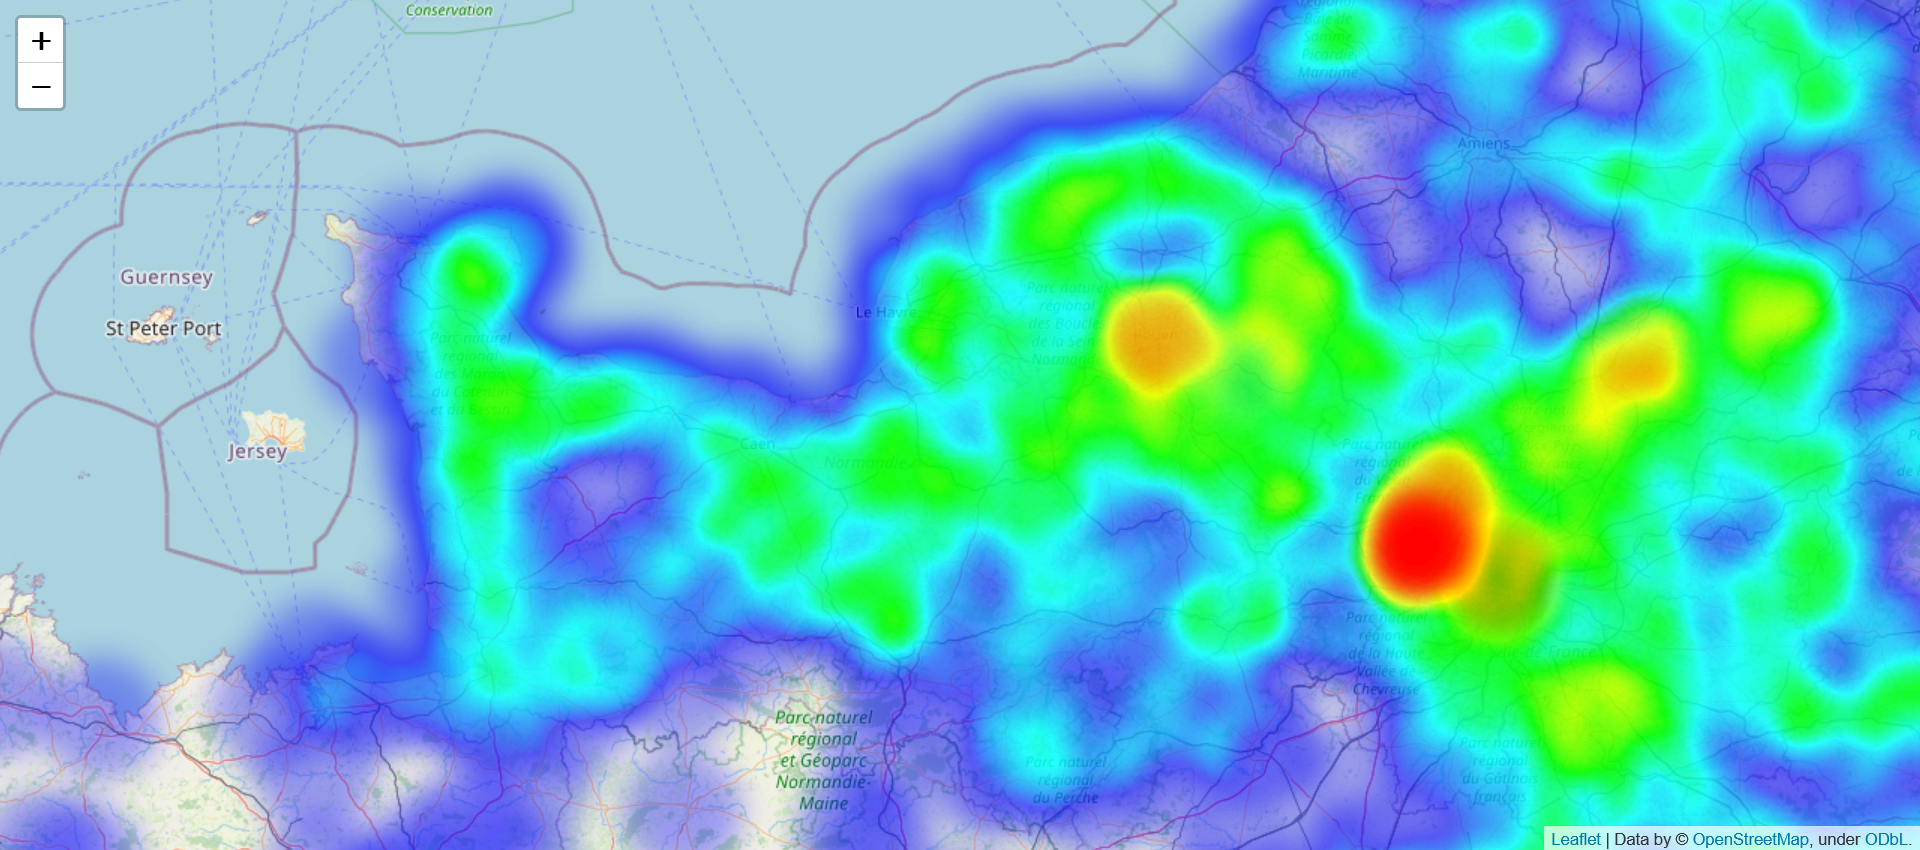
\includegraphics[width=\textwidth]{Images/Carte_zoom_Normandie.png}
		\caption{Carte des lieux mentionnés dans les registres JJ 37 à JJ 50 du Trésor des Chartes, zoom sur la Normandie.}
		\label{Carte_zoom_Normandie}
	\end{figure}
	
	\subsection{Cartographie intégrée à Heurist}
	
	La plateforme Heurist permet également de produire des visualisations cartographiques à partir des données géolocalisées en utilisant la même librairie javascript leaflet. L'interface offre de nombreuses possibilités car il est possible de trier les données en fonction des éléments que l'on veut observer en utilisant les jointures entre plusieurs tables. On peut par exemple visualiser les lieux mentionnés dans les actes où un nom précis apparaît (par exemple Enguerrand de Marigny pour la figure \ref{Carte_Enguerrand_Marigny}) ou visualiser les lieux contenus dans les actes réalisés pendant une période précise (par exemple au cours du pontificat de Benoît XI pour la figure \ref{Carte_Benoit_XI}). Ces requêtes jointes démultiplient ainsi les possibles études sur les liens entre des entités ou sur des collections d'actes du Trésor des chartes établis en fonction de critères précis.
	
	\begin{figure}
		\centering
		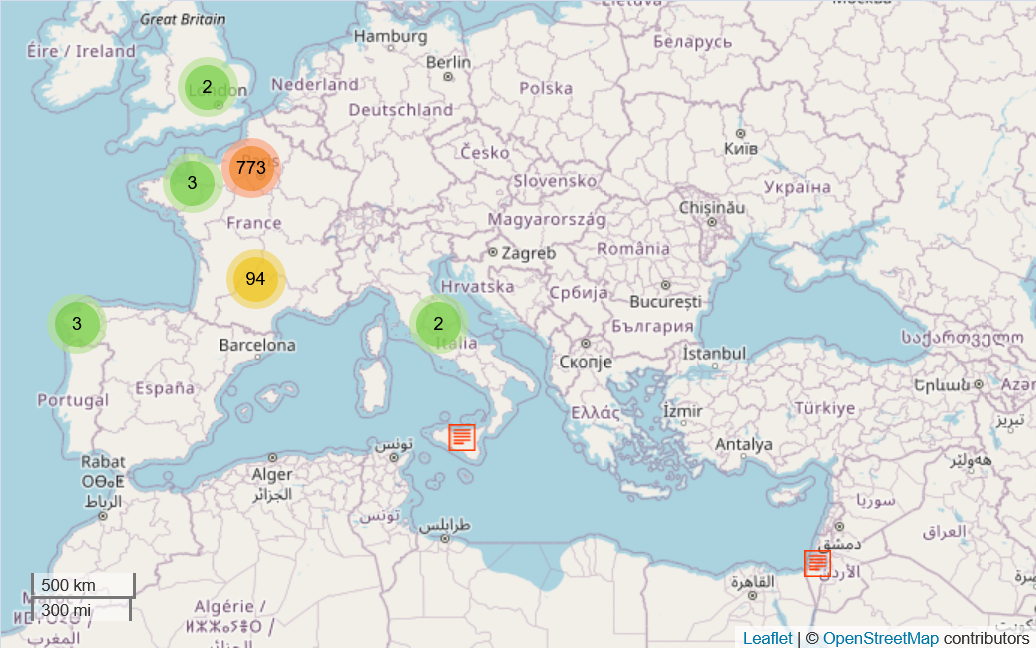
\includegraphics[width=\textwidth]{Images/Carte_Marigny.png}
		\caption{Carte des lieux mentionnés dans les actes contenant le nom d'Enguerrand de Marigny.}
		\label{Carte_Enguerrand_Marigny}
	\end{figure}

	\begin{figure}
		\centering
		\includegraphics[width=\textwidth]{Images/Carte_Benoît_XI.png}
		\caption{Carte des lieux mentionnés dans les actes réalisés pendant le pontificat de Benoît XI (27 octobre 1303 - 7 juillet 1304).}
		\label{Carte_Benoit_XI}
	\end{figure}
	
	\section{Import des actes sur Arkindex}
	
	\subsection{Les fonctionnalités de la plateforme}
	
	La dernière étape de la mise en ligne des données concerne la plateforme Arkindex utilisée pour l'entraînement des modèles de lecture automatique des textes. Les données issues de la segmentation en acte des registres transcrits ont en effet été intégrés dans un fichier JSON (\textit{cf}. Chapitre 2) et doivent être chargées dans la plateforme pour faire le lien entre le texte et les entités contenues dans la base de données. Cette étape a été réalisée à partir de la librairie python arkindex-client qui fournit un client API pour la plateforme \footnote{\url{https://pypi.org/project/arkindex-client}.}.
	
	L'utilisation de ces fonctions nécessite de déclarer au préalable des identifiants comme des variables d'environnement afin de se connecter à un compte Arkindex. Les différentes fonctions utilisables par l'API sont les suivantes : \url{https://arkindex.teklia.com/api-docs}. Dans le cadre de notre travail, nous avons utilisé la méthode \og paginate\fg{} dans le cadre des requêtes GET pour chercher des éléments dans un corpus Arkindex. Cette fonction de requête est particulièrement utile pour manipuler un grand nombre de données car le contenu est organisé dans des éléments \og Page\fg{} qui ne sont chargées qu'au moment où ils sont utilisés par le programme. Le retour est ensuite rassemblé dans un élément python ResponsePaginator et peut être manipulé et utilisé pour d'autres opérations. Les arguments utilisés pour les recherches sont \og ListElements \fg{} si on cherche des éléments en fonction d'un attribut ou \og ListElementChildren \fg{} si on cherche leurs éléments enfants.
	
	Les requêtes POST utilisent quant à elles la méthode \og request\fg{} et permettent d'envoyer du contenu dans la plateforme. Les arguments utilisés dépendent de l'action souhaitée : \og CreateElement\fg{} permet de créer un nouvel élément en renseignant son titre, son nom, l'identifiant du corpus et si besoin l'identifiant de l'élément parent ; \og CreateMetaData\fg{} permet de créer une métadonnée en renseignant son type, son nom, son contenu et l'identifiant de l'élément concerné ; \og CreateElementParent\fg{} permet de créer une relation enfant-parent en renseignant les identifiants des éléments enfants et parents concernés ; \og CreateTranscription\fg{} permet de créer une transcription en renseignant le texte et l'identifiant de l'élément concerné. Tous les contenus sont renseignés à l'aide d'un élément dictionnaire dont les clés correspondent au type de données nécessaires à l'établissement de l'action souhaitée.
	
	\subsection{L’objectif : Mettre en lien tous les éléments connus sur les images et les actes qu'elles contiennent}
	
	Dans ce cadre, nous avons donc élaboré en collaboration avec Teklia un script python permettant d'organiser l'import des données contenues dans le fichier JSON. L'algorithme se calque sur la structure du fichier que nous avons décrite au chapitre 2 (\textit{cf}. notamment figure \ref{json_final}) et itère des opérations successives avec l'API pour chaque élément correspondant à un acte. La première consiste à rechercher l'identifiant du volume dans lequel se trouve l'acte à l'aide de ListElements, puis à créer un élément Act comme enfant de ce volume avec CreateElement. CreateMetaData permet ensuite d'intégrer un à un les attributs de l'acte dans le fichier JSON comme métadonnée de l'élément Act selon la concordance suivante :
	
	\begin{center}
		\begin{tabular}{|p{8cm}|p{8cm}|}
			\hline
			Attribut dans le fichier JSON & Metadata dans Arkindex\\
			\hline\hline
			Provisory\_index\_3 & himanisId \\ \hline
			Inventory\_Name + '\_' + Inventory\_Nr & inventoryReference \\ \hline
			Regeste & abstract \\ \hline
			Date & date\_orig \\ \hline
			normalized\_language/language & language \\ \hline
		\end{tabular}
	\end{center}

	\noindent Une métadonnée supplémentaire \og date\fg{} est créée à partir de l'attribut \og Date-normalisee\fg{} transformé sous la forme YYYY-MM-DD s'il s'agit d'une date exacte ou YYYY-YYYY s'il s'agit d'un intervalle.
	
	Les zones de textes sont ensuite décrites sous forme d'un élément liste dans un attribut \og Text\_Region\fg{}. Ils permettent de décrire toutes les morceaux des actes au sein des pages. Leur modélisation au sein d'Arkindex doit donc prendre en compte leur situation d'interface entre la structure physique et structure logique des registres. Pour cette raison, nous avons d'abord cherché le nom du folio sur dans lequel se situe cette zone de texte à l'aide de l'adresse de l'image dans la BVMM et de la table de concordance entre les folios et les images que nous avons décrite au chapitre 6, puis nous avons cherché l'identifiant de ce folio dans Arkindex avec ListElements. Nous avons ensuite créé un élément Text zone comme enfant de ce folio à l'aide de CreateElement. L'élément est doté d'un nom qui reprend la valeur de l'attribut \og Act\_N\fg{} précédé de la chaîne \og Acte\fg{} et d'une image qui est la même que celle de l'élément parent découpée à partir du contenu de l'attribut \og Graphical\_coord\fg{}. Ces zones de texte sont aussi liées aux actes que nous avons importés précédemment, pour cette raison nous avons rajouté un lien enfant-parent depuis l'élément Text zone vers l'élément Act à l'aide de CreateElementParent. Nous avons pour finir utilisé CreateTranscription pour importer la transcription du texte contenu dans l'image et CreateMetaData pour intégrer la valeur de l'attribut \og type\_act{} comme Metadata \og part\fg{} selon la correspondance suivante :
	
	\begin{center}
		\begin{tabular}{|p{4cm}|p{4cm}|}
			\hline
			Valeur de l'attribut \og type\_act\fg{} & Valeur de la Metadata \og part\fg{}\\
			\hline\hline
			AI & initial \\ \hline
			AF & final \\ \hline
			AM & middle \\ \hline
			AS & supplemental \\ \hline
			AC & complete \\ \hline
		\end{tabular}
	\end{center}
	
	Cette situation permet aux éléments \og Text zone\fg{} d'être à la fois des enfants des éléments \og Page\fg{} et des éléments \og Act\fg{}. Ces derniers représentent donc le contenu intellectuel du texte et ne sont associés à aucune image par eux-mêmes. En revanche, il est possible de visualiser le contenu physique d'un élément \og Act\fg{} dans Arkindex à travers l'affichage successif de chacun des éléments \og Text zone\fg{} qu'il contient comme présenté par la figure \ref{Act_on_Arkindex}.
	
	\begin{figure}
		\centering
		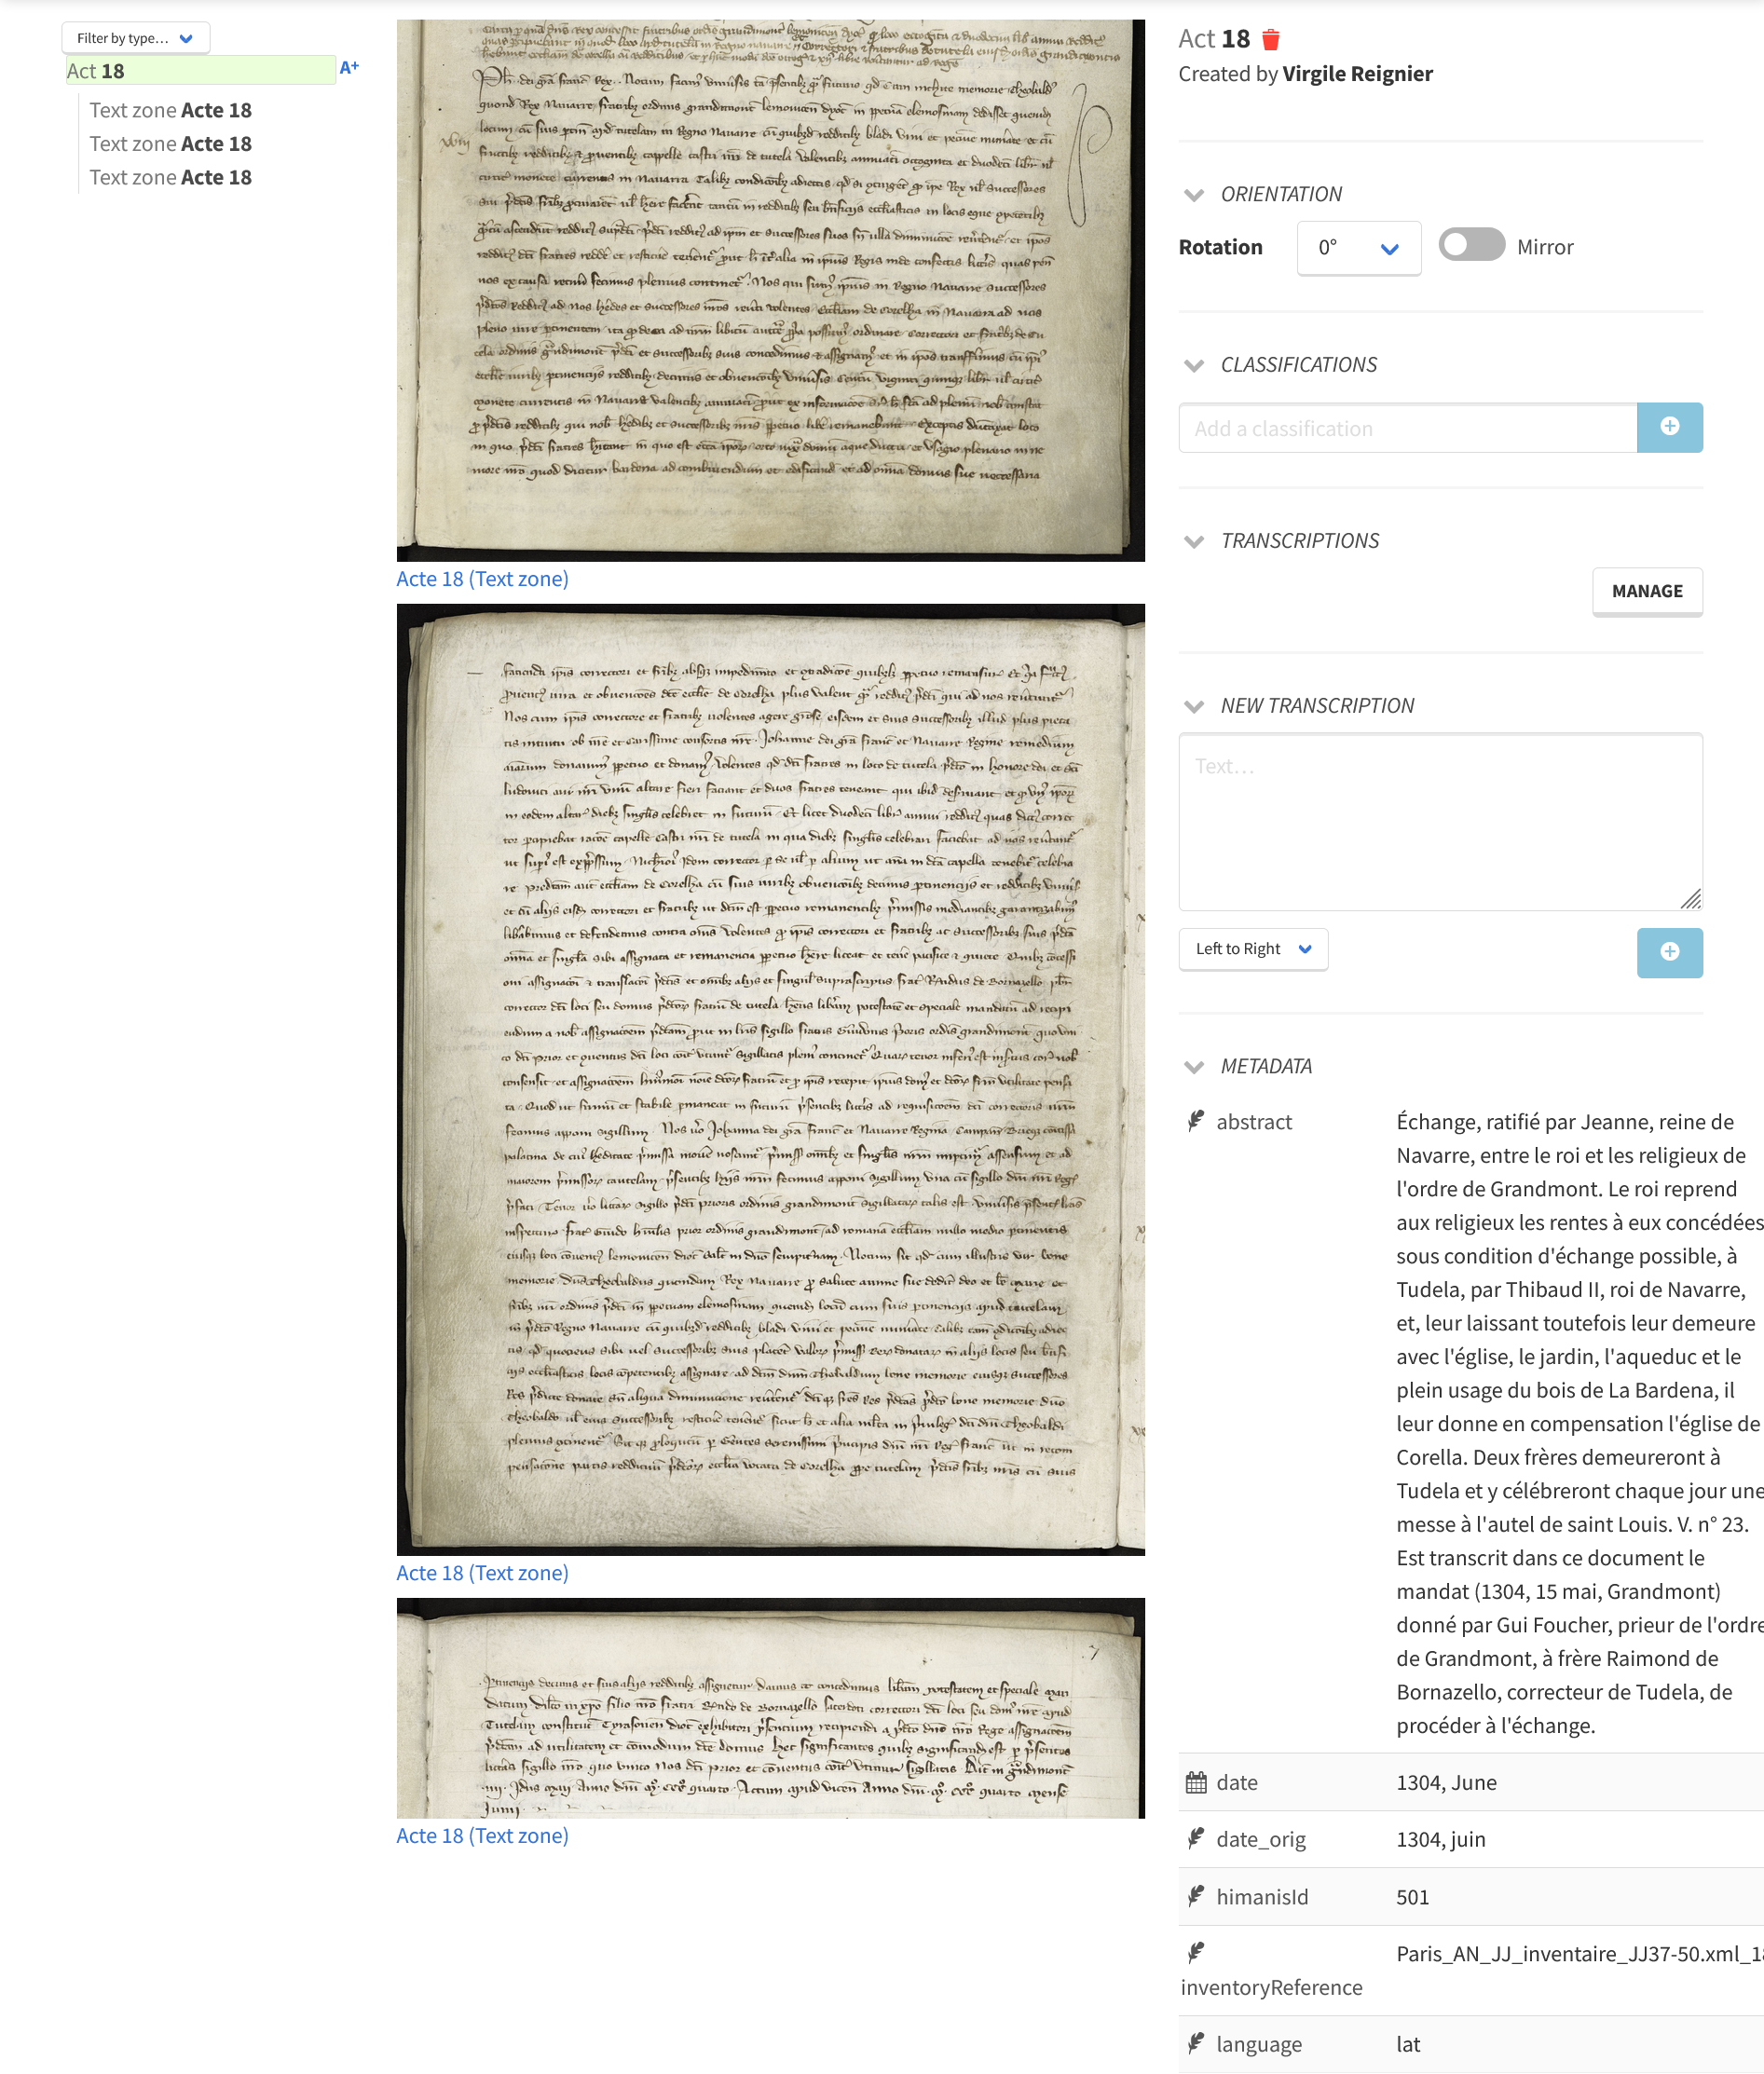
\includegraphics[width=12cm]{Images/Act_on_Arkindex.png}
		\caption{Visualisation d'un élément \og Act\fg{} dans Arkindex. Cet élément est le parent de plusieurs éléments \og Text zone\fg{} qui représentent chacun une portion du texte décrit par l'élément \og Act\fg{}.}
		\label{Act_on_Arkindex}
	\end{figure}

	De la même manière, nous avons mis en lien les éléments présents dans Heurist avec ceux chargés dans Arkindex. L'attribut \og Address bvmm\fg{} a notamment été modifié pour devenir du type \og File\fg{} ce qui permet de 
	
	Maintenant faut parler des images dans Heurist : visualisation des url d'images pour les zones d'image et intégration des id Arkindex pour les actes
	
	\section*{Conclusion}
	
	
	Du coup bah pour exploiter il faut que ce soit librement disponible, on va donc parler de Link Open Data !
	https://recherchemid.wordpress.com/2013/11/11/vous-avez-dit-linked-open-data/
	
	\chapter{Résultats du modèle développé}
	
	Tout ce qui suit ce sont des conseils de Lucence Ing, utile à garder pour le moment mais il faudra les supprimer.
	
	\chapter*{Conclusion générale}
	
	Pensée pour l'intro : dire que notre développement n'est pas linéaire car nous avons fait de nombreux aller-retour sur les étapes de notre travail en fonction que nous comprenions la complexité des données + certaines ont été anticipées. Du coup j'ai préféré un développement thématique
	
	Faire attention à l'emploi du "nous" -> Plus mettre en valeur ce que j'ai fait et mes choix dans le stage
	
	Dire aussi que j'ai fait un billet de blog et qu'on peut le lire en complément du mémoire
	
	
	Conseil : Tu peux créer des liens directement vers les parties mentionnées (ou sous-parties ?) en ajoutant un \ref ici et un \label après le titre du chapitre 4. C'est un peu fastidieux à faire mais ça fonctionne assez bien (avec le package hypersetup ou hyperref (les deu x fonctionnent) ;)
	
	Idée pour le chapitre 6 : faire un diagramme de flux pour illustrer le processus de construction de la BDR (à mettre dans une annexe ?)
	
	%les annexes
	\appendix
	\chapter{Les sous-entrées de \og Paris\fg{}}
	
	Comme on peut le voir dans les figures \ref{Paris_sous_entrée_1} et \ref{Paris_sous_entrée_2}, les sous-entrées de Paris sont complexes à interpréter de manière automatique. En effet, les séparateurs utilisés sont les mêmes au sein d'un même bloc, que celui-ci soit formé comme un ensemble de sous-sous-entrées dépendant d'une même sous-entrée ou tout simplement comme un ensemble de sous-entrées successives.
	
	\begin{figure}
		\centering
		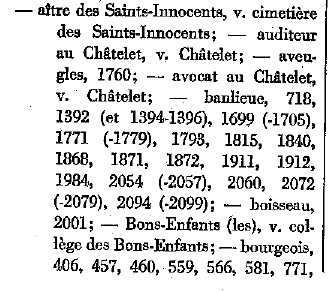
\includegraphics[width=\textwidth]{Images/Paris_sous_entrees_1.jpg}
		\caption{Ensemble de sous-entrée de \og Paris\fg{} dont les éléments sont rangés par ordre alphabétique.}
		\label{Paris_sous_entrée_1}
	\end{figure}

	\begin{figure}
		\centering
		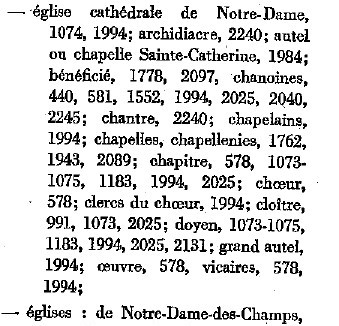
\includegraphics[width=\textwidth]{Images/Paris_sous_entrees_2.jpg}
		\caption{Ensemble de sous-entrée de \og Paris\fg{} dont les éléments sont des sous-sous-entrées dépendant de la sous-entrée \og église cathédrale de Notre-Dame\fg{}.}
		\label{Paris_sous_entrée_2}
	\end{figure}
	
	\chapter{Les erreurs natives dans l'index}
	
	Nous reportons ici différentes erreurs rencontrées au cours de notre travail. Les figures \ref{Parenthèses_pour_crochets} et \ref{Irregularité_crochets} sont des erreurs de typographie liées à l'absence d'un caractère ou à l'utilisation d'un caractère pour un autre. Les figures \ref{Marquage_non_systématique} et \ref{Erreur_alphabétique} sont des erreurs dans la systématicité des données liées à l'usage indifférent de plusieurs caractères pour signifier une même chose ou à l'ordonnancement des entrées.
	
	\pagebreak
	
	\begin{figure}
		\centering
		\includegraphics[width=\textwidth]{Images/Exemple_parenthèses.jpg}
		\caption{Contrairement à la forme utilisée tout au long de l'index, l'entrée \og Etrepagny\fg{} contient des indications géographiques entourées de parenthèses.}
		\label{Parenthèses_pour_crochets}
	\end{figure}
	
	\begin{figure}
		\centering
		\includegraphics[width=\textwidth]{Images/Exemple_irregularité.jpg}
		\caption{Déficit d'un crochet fermant.}
		\label{Irregularité_crochets}
	\end{figure}

	\begin{figure}
		\centering
		\includegraphics[width=\textwidth]{Images/Exemple_incohérence.jpg}
		\caption{Utilisation de deux caractères différents pour un même usage.}
		\label{Marquage_non_systématique}
	\end{figure}

	\begin{figure}
		\centering
		\includegraphics[height=\textheight]{Images/Erreur_alphabétique.jpg}
		\caption{\og Saint-Savin\fg{} est ici placé par erreur entre \og Saint-Omer\fg{} et \og Saint-Ouen\fg{}}
		\label{Erreur_alphabétique}
	\end{figure}
	
	\chapter{Suggestions pour l'amélioration du contenu de la base de données publiée sur Heurist}
	
	Malgré notre travail, la durée du stage ne nous a pas permis d'aller au bout de la formalisation du référentiel constitué à partir des entrées d'index. Pour que celui-ci soit pleinement utilisable, il faudrait encore améliorer certains éléments. Voici la liste de nos propositions : 
	
	\begin{enumerate}
		\item Les nom des entités issues de sous-entrées de l'index sont actuellement sous la forme \og Abandons , — spontanés au roi\fg{}. Si le séparateur \og  , — \fg{} nous a permis de repérer facilement ces entrées et de travailler sur leurs spécificités, ces noms pourraient être simplifié par son élimination systématique.
		
		\item Un tableau a été produit par les Archives Nationales à partir de la mise à plat de l'index des sujets. Dans le cadre de l'étape précédente, on peut envisager son usage comme référence pour les noms de sujet et proposer une fonction de comparaison automatique.
		
		\item Certaines marques de renvoi n'ont pas été prises en compte par les traitements réalisés, comme par exemple \og Agnès du Bois, femme de Guillaume de Flavacourt\fg{}. Guillaume de Flavacourt dispose bien d'une entrée à son nom dans l'index, mais la relation entre les deux entités reste à réaliser.
		
		\item La discrimination entre les éléments de la table Place et ceux de la table Person n'a pas pu être définie de manière parfaite. Il est donc probable qu'il demeure quelques incohérences parmi ces entrées.
		
		\item Les relations entre sous-entrées et entrées générales n'ont été qualifiés que pour la table des sujets. Pour la table des lieux et personnes, les sous-entrées dépendant d'entrées catégorisées comme des lieux ont toutes été transformées de la même façon indépendamment de leur contenu. Elles forment donc toutes des entrées de la table Place. De la même manière, toutes les sous-entrées dépendant d'entrées catégorisées comme des personnes ont été transformées comme des description de la relation entre l'entrée principale et les entrées d'inventaire associées à ces sous-entrées. La catégorisation de ces sous-entrées permettrait donc d'améliorer largement l'utilisation de ces données.
		
		\item Lorsque les circonscriptions administratives auxquelles sont rattachés les éléments de la table Place disposent elles aussi d'une entrée dans cette même table, il serait envisageable de créer une relation entre ces deux entrées.
		
		\item Certaines entrées de la table Place disposant de plusieurs propositions de localisation sont en réalité des erreurs. Par exemple l'entrée \og Bruetel (maison de) [région de Marigny, Seine-Maritime, con Gournay, cne Dampierre]\fg{} a été aligné avec les deux communes nommées Dampierre dans le département de la Seine-Maritime alors que l'une d'elle n'est pas située dans le canton de Gournay et aurait pu être éliminée des propositions de localisations. Ces données comme le script utilisé pour l'alignement peuvent donc être améliorés à cet effet.
		
		\item Les marques d'incertitude qui sont décrits dans la colonne \og incertitude\fg{} du fichier geonames\_final.csv n'ont pas été reportés dans la base de données. La prise en compte de ces incertitudes, ainsi que des marques présentes dans les autres types d'entrées (notamment les \og ?\fg{}) est donc encore à réaliser.
		
		\item Les entrées pour lesquelles l'index propose plusieurs localisation ont été dédoublées dans le fichier geonames\_final.csv. Mais seule l'une des propositions a été importée dans la base de données. L'import des autres propositions reste donc à réaliser.
		
		\item Les éléments insérés parmi les renvois vers les entrées d'inventaire, comme par exemple les références à la section \og Additions et corrections\fg{}, n'ont pour le moment pas été pris en compte.
		
		\item Actualiser le nom de départements des entités situées dans les anciens départements de la Seine et Seine-et-Oise.
		
	\end{enumerate}
	
	\backmatter
	\phantomsection
	\addcontentsline{toc}{chapter}{\listfigurename}
	\listoffigures
	\tableofcontents
	
\end{document}